\documentclass[doublespace,Afour,sageh,times]{sagej}
\usepackage{amsmath,amssymb,amsthm,graphicx,booktabs,array,url}
\usepackage[colorlinks,bookmarksopen,bookmarksnumbered,citecolor=blue,urlcolor=blue]{hyperref}
\setcounter{secnumdepth}{3}
\setcounter{dbltopnumber}{2}
\renewcommand{\dbltopfraction}{0.85}
\def\journalname{The International Journal of Robotics Research}
\runninghead{Supplementary derivations and experiments}
\newtheorem{theorem}{Theorem}
\newtheorem{proposition}[theorem]{Proposition}
\newtheorem{lemma}[theorem]{Lemma}
\newtheorem{corollary}[theorem]{Corollary}
\theoremstyle{definition}
\newtheorem{assumption}{Assumption}
\newtheorem{remark}{Remark}
\newcommand{\R}{\mathbb R}
\newcommand{\C}{\mathbb C}
\newcommand{\T}{\mathbb T}
\newcommand{\dd}{\,\mathrm d}
\newcommand{\norm}[1]{\left\lVert#1\right\rVert}
\newcommand{\abs}[1]{\left|#1\right|}
\newcommand{\diag}{\operatorname{diag}}
\newcommand{\Rea}{\operatorname{Re}}
\newcommand{\Ima}{\operatorname{Im}}
\newcommand{\eps}{\varepsilon}
\providecommand{\doi}[1]{\href{https://doi.org/#1}{doi: #1}.}

\renewcommand{\thesection}{S\arabic{section}}
\renewcommand{\theequation}{S\arabic{equation}}
\renewcommand{\thetheorem}{S\arabic{theorem}}
\renewcommand{\theassumption}{S\arabic{assumption}}
\renewcommand{\theremark}{S\arabic{remark}}
\renewcommand{\thetable}{S\arabic{table}}
\renewcommand{\thefigure}{S\arabic{figure}}
\begin{document}
\title{Supplementary material: Complex Hamiltonian learning and KAM-preserving magnetic control of a catheter model}
\author{Anonymous authors}
\begin{abstract}
This supplement gives the distributed force accounting, complete learning-error estimates, nonlinear normal forms, invariant-torus proofs and extended numerical experiments supporting the main article. It also supplies the full magnetic-feedback lift, energy-based clearance proofs and explicit local KAM measure calculation. Numerical observations and infinite-time conclusions retain their respective domains and assumptions. External theorems are attributed at their point of application; model-specific derivations and proofs are included here.
\end{abstract}
\maketitle
\raggedbottom
\section{Distributed mechanics and the unified magnetic model}
\label{sec:mechanics}
% Integration fragment; theorem/proof environments must be defined by the host.
% All variables in the learning and safety subsections are dimensionless.

\subsection{Rod mechanics and a variationally consistent reduction}
Following the spatial rod formulation \citep{simo,antman}, let $s\in[0,L]$ denote reference arclength, $r(s,t)\in\mathbb R^3$
the centreline and $D(s,t)\in SO(3)$ its director frame. Define
\begin{equation}
 \Gamma=D^{\mathsf T}r_s,\quad
 D_s=D\widehat\kappa,\quad D_t=D\widehat\omega_b.
\end{equation}
The hat map is defined by $\widehat a b=a\times b$.
The extensible, unshearable Kirchhoff specialization has
$\Gamma=(0,0,1+e)^{\mathsf T}$; inextensibility additionally sets $e=0$.
Transverse internal forces are then constraint reactions. They must not
be set to zero by substituting zero shear into a shearable constitutive law.
In spatial components the balances are
\begin{align}
 \rho A r_{tt}&=n_s+f_{\rm mag}+f_{\rm h}+f_{\rm c}+\rho A g,\\
 \partial_t(D\mathcal J_b\omega_b)&=m_s+r_s\times n+\tau_{\rm ext}.
\end{align}
For constant body inertia, the left side of the second equation is
$D(\mathcal J_b\dot\omega_b+\omega_b\times\mathcal J_b\omega_b)$.
With stored energy density $W(\Gamma,\kappa)$, unconstrained components
of $D^{\mathsf T}n$ and $D^{\mathsf T}m$ are its strain derivatives.
A fixed base specifies position and orientation; a free tip specifies
the appropriate force and moment resultants, including any concentrated
magnetic load.

For a body-fixed magnetic moment density $\mu_b(s)$ and a static applied
field $B_0(r)$, neglecting magnetic interactions between distinct
material elements gives the applied-field potential
\begin{equation}
 V_{\rm mag}=-\int_0^L(D\mu_b)\cdot B_0(r)\,ds.
\end{equation}
Its translational and rotational variations give
$f_{\rm mag}=\nabla_r(\mu\cdot B_0)$ at fixed orientation and
$\tau_{\rm mag}=\mu\times B_0$, where $\mu=D\mu_b$.
Thus static magnetic loading belongs to the conservative energy.
Field modulation supplies explicit time-dependent work or an input port.
The permanent-dipole load is the leading term of the Maxwell-stress
resultant derived below; it is counted once in the force balance.

For a complete localized magnetic element, the magnetostatic force
can be evaluated on a surrounding vacuum control surface $\Sigma$:
\begin{equation}
 F_{\rm mag}=\int_\Sigma T_Mn_\Sigma\dd A,\qquad
 T_M=\mu_0^{-1}(BB^{\mathsf T}-\tfrac12|B|^2I).
\end{equation}
Here $B$ is the total field, including the element's self-field.
The associated moment integrates the moment arm crossed with
$T_Mn_\Sigma$. To recover the permanent-dipole approximation, represent
the element by its complete localized steady current $j(\xi)$,
including bound currents, with $\xi=x-r$. The prescribed magnetization
is unaffected by the applied field $B_{\rm ext}$, whose sources lie
outside $\Sigma$. Current closure gives $\nabla\cdot j=0$ and no flux
through the boundary. The identity $\nabla\cdot T_M=j\times B$ and
symmetry of $T_M$ convert the stress resultants into Lorentz force and
moment. The self-field has zero net force and moment, as seen by taking
its stress surface to infinity; the applied-field-only stress also has
zero resultant in this source-free volume. The remaining interaction is
\begin{equation}
\begin{aligned}
 m_{\rm d}&=\tfrac12\int\xi\times j(\xi)\,\dd V,\\
 F_{\rm mag}&=\int j(\xi)\times B_{\rm ext}(r+\xi)\,\dd V\\
 &=\nabla_r\!\left(m_{\rm d}\cdot B_{\rm ext}(r)\right)+R_F,\\
 \tau_{\rm mag}&=\int\xi\times[j(\xi)\times B_{\rm ext}(r+\xi)]\,\dd V\\
 &=m_{\rm d}\times B_{\rm ext}(r)+R_\tau .
\end{aligned}
\label{eq:stress-dipole-reduction}
\end{equation}
The gradient holds the moment orientation fixed.
Integration by parts gives $\int j\,\dd V=0$ and
$\int\xi_i j_j\,\dd V=\epsilon_{ijk}(m_{\rm d})_k$.
Taylor expansion of $B_{\rm ext}$ and $\nabla\cdot B_{\rm ext}=0$
then give \eqref{eq:stress-dipole-reduction}.
For $J_2=\int|\xi|^2|j(\xi)|\,\dd V$, the remainders obey
$|R_F|\le\tfrac12J_2\sup\|D^2B_{\rm ext}\|$ and
$|R_\tau|\le J_2\sup\|DB_{\rm ext}\|$, with operator norms taken over
the element and its Taylor segments. Surface-current contributions are
included in these integrals when present. Neglecting the higher
multipoles recovers the permanent-dipole force and torque used in
magnetic robotics \citep[Section~4.1, Eqs.~(12) and~(16)]{abbott}.

A modified Morison-type local closure, stated per unit reference length,
is
\begin{align}
 f_{\rm h}={}&m_f a_f+m_a(a_f-r_{tt})
             -c_1v_r-c_2|v_r|v_r,\\
 v_r={}&r_t-v_f,\qquad c_1,c_2\ge0.
\end{align}
Here $m_f=\rho_f A_f$ and $m_a$ are displaced-fluid and added mass
per unit length; $a_f$ is the prescribed fluid acceleration.
This is a reduced closure requiring calibration, not a solved
Navier--Stokes interaction. In still fluid its drag power is
$-c_1|r_t|^2-c_2|r_t|^3$. In moving fluid it is dissipative relative to
the fluid velocity and can do positive work on the rod. A constant
added mass may be moved to the inertial side exactly once.

For a stationary wall, define penetration $\delta(r)$ positive inside
the wall and $n_c=\nabla\delta$. One nonadhesive penalty model is
\begin{align}
 V_c&=\frac{k_c}{m+1}[\delta]_+^{m+1},\\
 f_c&=-k_c[\delta]_+^m n_c
       -c_c\mathbf1_{\{\delta>0\}}[\dot\delta]_+n_c.
\end{align}
The elastic term is included through $V_c$ and the second term dissipates
power during compression. Friction can be added as a dissipative port.
This switching law is used for force accounting outside the contact-free
KAM domain, not as an analytic perturbation through an impact.

Choose a configuration map $(r(s,q),D(s,q))$ that satisfies the essential
boundary conditions and the rod constraints. A linear centreline
ansatz alone is insufficient to specify rotational inertia. Define
\begin{equation}
 r_i=\partial_{q_i}r,\qquad
 a_i=\operatorname{vee}(D^{\mathsf T}\partial_{q_i}D).
\end{equation}
Then $\omega_b=\sum_i a_i\dot q_i$ and the reduced kinetic energy is
\begin{align}
 T_N&=\tfrac12\dot q^{\mathsf T}M(q)\dot q,\\
 M_{ij}(q)&=\int_0^L\left(\rho A r_i\cdot r_j+
                 a_i^{\mathsf T}\mathcal J_ba_j\right)ds.
\end{align}
An added-fluid-mass contribution may be included when its consistent
kinetic metric and associated inertial terms are specified. Otherwise
hydrodynamic inertia remains in the generalized force balance and is
not also included in $M$. Galerkin projection of the virtual-work
identity gives
\begin{equation}
 M(q)\ddot q+C(q,\dot q)\dot q+\nabla V_N(q)=Q_{\rm nc},
\end{equation}
\begin{equation}
 Q_i=\int_0^L(f\cdot r_i+\tau\cdot Da_i)ds+Q_i^\partial.
\end{equation}
Here $C\dot q$ denotes the Christoffel contribution of $M$, and $V_N$
contains elastic, static magnetic and retained gravitational potentials.
Microgravity reduces the last contribution; it does not eliminate
fluid drag or establish a particular blood-flow profile.
Relative-flow drag, moving-base work and contact losses are retained in
$Q_{\rm nc}$. A stationary-fluid quadratic drag, for example, has
nonpositive power; a moving fluid may inject energy. Contact switching
is excluded from the analytic neighbourhood used for KAM analysis.

For $M(q)\succ0$, the Legendre transform yields
\begin{equation}
 p=M(q)\dot q,\qquad
 H_N(q,p)=\tfrac12p^{\mathsf T}M(q)^{-1}p+V_N(q).
\end{equation}
In particular,
$\dot p_i=-\tfrac12p^{\mathsf T}\partial_{q_i}(M^{-1})p
-\partial_{q_i}V_N+(Q_{\rm nc})_i$.
The configuration dependence of inertia is retained. Potential forces
appear either in $V_N$ or in $Q_{\rm nc}$, never both.

\subsection{Complex energy--dissipation representation with an explicit decoder}
Energy and Rayleigh dissipation have different physical units. Let $E_0$
and $t_0$ be reference energy and time, and choose diagonal position and
momentum scales $Q_0,P_0$ with $Q_0^{\mathsf T}P_0=E_0t_0I$.
Set $q=Q_0x$, $p=P_0y$, $\tau=t/t_0$ and
\begin{align}
 h(x,y)&=H_N(Q_0x,P_0y)/E_0,\\
 d(x,v)&=\frac{t_0}{E_0}\mathcal D_N(Q_0x,Q_0v/t_0).
\end{align}
Here $v=dx/d\tau$ and $\mathcal D_N$ is a Rayleigh dissipation potential.
The two entries of $h+id$ are now dimensionless. A complex network
provides coupled features and two physically decoded real readouts,
\begin{align}
 \mathcal H_\theta(x,y,v)&=h_\theta(x,y)+i d_\theta(x,v),\\
 h_\theta&=h_{\rm prior}+h_{{\rm res},\theta}.
\end{align}
One admissible dissipative head is
\begin{equation}
 d_\theta(x,v)=\tfrac12v^{\mathsf T}D_\theta(x)v,
 \qquad D_\theta(x)=L_\theta(x)L_\theta(x)^{\mathsf T}\succeq0.
\end{equation}
More general heads may be used if $d_\theta(x,\cdot)$ is differentiable,
convex and minimized at zero. The decoder is
\begin{align}
 v&=\partial_y h_\theta,\qquad x'=v,\\
 y'&=-\partial_x h_\theta-\partial_vd_\theta(x,v)+B(x)u.
 \label{eq:fragment-decoder}
\end{align}
The derivative of $d_\theta$ is taken with respect to its independent
velocity argument before substituting $v=\partial_yh_\theta$.
It is not a total derivative through this substitution.

\begin{proposition}[Power-consistent complex representation]
For a differentiable $h_\theta$, the decoded system satisfies
\begin{equation}
 \frac{d h_\theta}{d\tau}
 =-v^{\mathsf T}\partial_vd_\theta(x,v)
   +u^{\mathsf T}B(x)^{\mathsf T}v+\partial_\tau h_\theta.
 \label{eq:fragment-power}
\end{equation}
For the quadratic head, the first term equals
$-v^{\mathsf T}D_\theta(x)v\le0$. For the convex head it is also
nonpositive.
\end{proposition}
\begin{proof}
Apply the chain rule to $h_\theta$ and substitute
\eqref{eq:fragment-decoder}. The two canonical terms cancel.
Convexity and the minimum at zero imply
$v^{\mathsf T}\partial_vd_\theta(x,v)
\ge d_\theta(x,v)-d_\theta(x,0)\ge0$.
\end{proof}

With $z=(x+iy)/\sqrt2$, the canonical convention is
$\{z_j,\bar z_k\}=-i\delta_{jk}$ and
\begin{equation}
 z'=-i\partial_{\bar z}h_\theta
       -\frac{i}{\sqrt2}\partial_vd_\theta
       +\frac{i}{\sqrt2}B(x)u.
\end{equation}
This is a unified complex representation of conservative and
nonconservative dynamics with a specified physical decoder. The rule
$z'=-i\partial_{\bar z}(h_\theta+i d_\theta)$ would generally produce
a different vector field and has no automatic dissipativity guarantee.
Real analyticity in $(x,y)$, and a controlled analytic extension to a
complex neighbourhood, are the relevant requirements for analytic KAM.
Holomorphicity in $z$ alone is not required of a nonconstant real energy
$h_\theta(z,\bar z)$. In particular, ReLU or modReLU features require a
separate smooth approximation or a theorem of appropriate regularity;
their ordinary piecewise-smooth implementation is not analytic.


The dimensional specialization below uses explicit SI units. The learning
and KAM statements use dimensionless canonical variables, with their
energy and time scales declared before fitting.

\subsection{One clamped--free magnetic beam throughout the computational study}
\label{sec:unified-model}
We instantiate the rod reduction as a straight, planar, small-slope
Euler--Bernoulli cantilever with a concentrated magnetic dipole at its free
tip. The base position and slope are fixed. The elastic part is linear in
curvature; the full trigonometric magnetic potential is retained. These
choices define a reproducible mechanical specialization of the spatial
rod, rather than a catheter-specific material identification. Table~\ref{tab:unified-si}
states all dimensional parameters. Gravity, imposed fluid flow and field
gradient are zero in this specialization. Still-fluid/structural losses
are represented by a mass-proportional Rayleigh term. The more general
force accounting above remains applicable when those terms are present.

\begin{table}[t]
\centering
\caption{Declared parameters of the unified magnetic cantilever. These are
illustrative mechanical parameters, not measurements from a clinical or
spaceflight device.}
\label{tab:unified-si}
\setlength{\tabcolsep}{3pt}
\begin{tabular}{lll}
\toprule
Quantity & Symbol & Value\\
\midrule
Length & $L$ & $0.08\,\mathrm m$\\
Circular radius & $r_c$ & $0.0006\,\mathrm m$\\
Young's modulus & $E$ & $5.0\times10^6\,\mathrm{Pa}$\\
Density & $\rho$ & $1100\,\mathrm{kg\,m^{-3}}$\\
Tip dipole & $\mu$ & $2.0\times10^{-5}\,\mathrm{A\,m^2}$\\
Axial bias field & $B_0$ & $0.03\,\mathrm T$\\
Mass damping rate & $\alpha$ & $0.55558524\,\mathrm{s^{-1}}$\\
Transverse field amplitude & $B_a$ & $0.006\,\mathrm T$\\
Drive frequency & $\Omega_d$ & $9.4449490\,\mathrm{rad\,s^{-1}}$\\
Ramp time & $t_r$ & $0.25\,\mathrm s$\\
Uniform Hermite elements & $N_e$ & $32$\\
\bottomrule
\end{tabular}
\end{table}

Write $w(s,t)$ for transverse displacement and
$\vartheta(t)=w_s(L,t)$ for the small-slope tip rotation. A uniform field
$(B_0,B_y(t))$ has zero translational dipole force and the tip moment
\begin{equation}
 M_{\rm tip}=\mu\{B_y(t)\cos\vartheta-B_0\sin\vartheta\}.
 \label{eq:unified-tip-torque}
\end{equation}
This is the natural moment boundary load. It does not impose a second
kinematic constraint at the free tip. The magnetic potential is
$-\mu(B_0\cos\vartheta+B_y\sin\vartheta)$, so that
\eqref{eq:unified-tip-torque} follows by variation. Keeping this potential
exact does not remove the small-slope approximation in the beam kinematics.

Let $q=(w_1,\vartheta_1,\ldots,w_{N_e},\vartheta_{N_e})^{\mathsf T}$
contain the unconstrained cubic-Hermite nodal coordinates, $e_\vartheta$
select its final rotation, and $M,K$ be the consistent mass and bending
stiffness matrices. The physical equations and static-bias energy are
\begin{align}
 M\ddot q+\alpha M\dot q+Kq
 &=e_\vartheta M_{\rm tip},
 \label{eq:unified-fe}\\
 H_0(q,p)&=\tfrac12p^{\mathsf T}M^{-1}p+\tfrac12q^{\mathsf T}Kq\notag\\
 &\quad+E_0\{1-\cos(e_\vartheta^{\mathsf T}q)\},
 \label{eq:unified-SI-H}\\
 E_0&=\mu B_0=6\times10^{-7}\,\mathrm J,\qquad p=M\dot q.
\end{align}
There is no axial end restraint and no artificial stretching quartic.
The nonlinearity used in learning and in the KAM calculation is the
magnetic nonlinearity of this same cantilever.

The static-field linearization is
$K_b=K+E_0e_\vartheta e_\vartheta^{\mathsf T}$.
Choose $\Phi^{\mathsf T}M\Phi=I$ and
$\Phi^{\mathsf T}K_b\Phi=\operatorname{diag}(\omega_j^2)$,
with positive tip-slope entries fixing modal signs. For $n$ retained modes,
$q=\Phi_n a$, and the modal momentum is $\pi=\dot a$.
Set $\omega_0=\omega_1$, $\tau=\omega_0t$, $\nu_j=\omega_j/\omega_0$,
and
\begin{equation}
 a_j=\sqrt{\frac{E_0}{\omega_0\omega_j}}X_j,
 \qquad
 \pi_j=\sqrt{\frac{E_0\omega_j}{\omega_0}}Y_j.
 \label{eq:unified-scale}
\end{equation}
The product of each position--momentum scale is $E_0/\omega_0$;
division of energy by $E_0$ and rescaling time therefore give the standard
dimensionless canonical equations. Define
\begin{equation}
 S=\Phi_n\operatorname{diag}\sqrt{\frac{E_0}{\omega_0\omega_j}},
 \quad d=S^{\mathsf T}e_\vartheta,\quad
 \ell(s)^{\mathsf T}=N(s)S,
\end{equation}
where $N(s)$ is the Hermite displacement row. Thus the full centreline
and tip slope are recovered in SI units as
$w(s)=\ell(s)^{\mathsf T}X$ and $\vartheta=d^{\mathsf T}X$.
The single dimensionless Hamiltonian used below is
\begin{align}
 h_*(X,Y)&=h_2(X,Y)+R_{\rm mag}(X),\\
 h_2&=\tfrac12\sum_{j=1}^n\nu_j(X_j^2+Y_j^2),\\
 R_{\rm mag}&=1-\cos(d^{\mathsf T}X)-\tfrac12(d^{\mathsf T}X)^2.
 \label{eq:unified-h}
\end{align}
The subtracted quadratic avoids counting the static magnetic stiffness
twice. For the two-mode model,
$(\omega_1,\omega_2)=(11.41728728,70.24049294)\,\mathrm{rad\,s^{-1}}$.
All learned models use this fixed chart; states are not independently
renormalized after fitting.

With $u=B_y/B_0$, $\gamma=\alpha/\omega_0$ and
$\mathsf N=\operatorname{diag}(\nu_j)$, the physical port decoder becomes
\begin{align}
 X'&=\partial_Y h,\\
 Y'&=-\partial_X h-\gamma\mathsf N^{-1}\partial_Yh
          +u\,d\cos(d^{\mathsf T}X).
 \label{eq:unified-port}
\end{align}
For $h=h_*$, the damping term is exactly $-\gamma Y$.
The Rayleigh head is
$\mathcal D(v)=\tfrac12\gamma v^{\mathsf T}\mathsf N^{-1}v$.
For a learned energy, retaining the velocity-based form in
\eqref{eq:unified-port} preserves nonnegative dissipation. Using
$-\gamma Y$ after learning a momentum-dependent residual would, in
general, lose that guarantee. The corresponding power identity is
\begin{equation}
 h'=-\gamma(\partial_Yh)^{\mathsf T}\mathsf N^{-1}\partial_Yh
       +u\cos(d^{\mathsf T}X)d^{\mathsf T}\partial_Yh.
 \label{eq:unified-power}
\end{equation}
Alternatively, including $-u\sin(d^{\mathsf T}X)$ in the time-dependent
energy moves the input power to $-u'\sin(d^{\mathsf T}X)$.
These are equivalent bookkeeping conventions.

\subsection{Independent COMSOL realization of the same discretization}
The model was also constructed and solved in COMSOL Multiphysics
6.3.0.290 through LiveLink for MATLAB. Its two-dimensional Beam interface
uses the Euler--Bernoulli formulation, 32 uniform elements, a consistent
mass matrix, a fixed base, and the nonlinear tip moment
\eqref{eq:unified-tip-torque}. Geometric nonlinearity is disabled to match
the declared small-slope mechanical model. The zero axial displacement
subspace decouples, leaving 64 transverse displacement/rotation degrees
of freedom.

After selecting transverse degrees of freedom by their field names and
coordinates, the independently assembled COMSOL and Python mass and
elastic stiffness matrices have relative Frobenius differences
$7.76\times10^{-15}$ and $3.05\times10^{-14}$, respectively. The first
six modal frequencies agree to a maximum relative difference of
$1.88\times10^{-9}$. These checks establish agreement of the stated
discretizations; they do not establish the material validity of the
chosen parameters. The native model, assembly exports, parameter values
and time-domain verification records accompany the manuscript.

\subsection{A global result for the unforced physical model}
\begin{proposition}[Unforced global stability of the full FE target]
\label{prop:unified-global-stability}
For the full clamped--free Hermite model~\eqref{eq:unified-SI-H}, set
$B_y=0$. With the declared parameters, the potential is globally
strongly convex and the origin is its unique equilibrium.
If $\alpha>0$, the origin is globally asymptotically stable.
If $\alpha=0$, every finite-energy trajectory remains in a bounded
energy sublevel and the origin is Lyapunov stable.
These are global statements for the declared small-slope mathematical
model; they do not establish its physical validity at large deflections
or a global property of arbitrary learned quartic residuals.
\end{proposition}

\begin{proof}
Write $b=e_\vartheta$ and
$U(q)=q^{\mathsf T}Kq/2+E_0\{1-\cos(b^{\mathsf T}q)\}$.
The clamped conditions give
$|w_s(L)|^2\leq L\int_0^L|w_{ss}|^2\,ds$, including for every
Hermite finite-element function. Equivalently,
$bb^{\mathsf T}\preceq [L/(EI)]K$; equality of the corresponding
tip compliance follows from the static quadratic bending shape.
Thus, for every $q$,
\begin{align}
 D^2U(q)&=K+E_0\cos(b^{\mathsf T}q)bb^{\mathsf T}\notag\\
 &\succeq(1-\kappa)K\succeq0.905K,\\
 \kappa&=\frac{E_0L}{EI}=\frac8{27\pi}<0.095.
\end{align}
In particular, $\nabla U=0$ only at $q=0$.
Both $M$ and $K$ are positive definite, and
\[
 H_0\geq\tfrac12p^{\mathsf T}M^{-1}p+\tfrac12q^{\mathsf T}Kq.
\]
Its sublevels are compact. Along the unforced dynamics,
\[
 \dot H_0=-\alpha p^{\mathsf T}M^{-1}p\leq0.
\]
This proves boundedness, global continuation and Lyapunov stability.
For $\alpha>0$, the largest invariant set with $\dot H_0=0$ has
$p=0$ and $\nabla U(q)=0$, hence consists only of the origin.
LaSalle's invariance principle on each compact sublevel gives global
asymptotic stability.
\end{proof}

\section{Complex Hamiltonian learning}
\label{sec:learning}
\subsection{A fixed canonical chart}
For a positive definite constant mass $M$ and reference stiffness $K_{\rm ref}$, select $U$ such that $U^{\mathsf T}MU=I$ and $U^{\mathsf T}K_{\rm ref}U=\Omega^2$, where $\Omega=\diag(\omega_1,\ldots,\omega_n)$. In the magnetic specialization, $K_{\rm ref}=K_b$ includes the static-field stiffness. The transformation
\begin{equation}
 q=U\Omega^{-1/2}Q,\qquad p=MU\Omega^{1/2}P
 \label{eq:balancechart}
\end{equation}
is symplectic: its configuration and momentum blocks satisfy $S_q^{\mathsf T}S_p=I$. Consequently $H_2=\tfrac12\sum_j\omega_j(Q_j^2+P_j^2)$. The computational variables in \eqref{eq:unified-scale} obey $(Q,P)=\sqrt{E_0/\omega_0}(X,Y)$, together with the stated energy and time normalization. That fixed dimensionless chart is used for training, derivative errors and normal forms. Canonical normalization requires the position and momentum scalings to preserve the symplectic form. Optional training weights change only the loss metric.

Write $x=(Q,P)$ and use one complex normalization throughout:
\begin{equation}
 z_j=\frac{Q_j+iP_j}{\sqrt2},\quad I_j=z_j\bar z_j,
 \qquad\{z_j,\bar z_k\}=-i\delta_{jk}.
 \label{eq:complexchart}
\end{equation}
Wirtinger calculus gives $\partial_{\bar z_j}=(\partial_{Q_j}+i\partial_{P_j})/\sqrt2$ and therefore $\dot z=-i\partial_{\bar z}H$ for real $H$. This is a change of representation of a real symplectic system. Holomorphicity in $z$ alone would exclude most real energy functions, including $H_2=\sum_j\omega_jz_j\bar z_j$. The analyticity required by analytic KAM instead means a holomorphic extension of the real variables $(Q,P)$ to a complex neighbourhood, in which $z$ and $\bar z$ are independent linear combinations.

\subsection{Architecture and objective}
A shared complex feature map $F_\theta(z,\bar z,b)$, with magnetic configuration $b$, drives real readouts for $H_\theta$ and a dissipation factor $L_\theta$. The latter defines $\mathcal D_\theta(q,v)=\tfrac12\norm{L_\theta(q)^{\mathsf T}v}^2$. The physical decoder in Section~\ref{sec:mechanics} determines the vector field. An affine complex layer has the real block realization
\begin{equation}
 (A+iB)(a+ib)= (Aa-Bb)+i(Ba+Ab).
 \label{eq:block}
\end{equation}
Thus complex weights impose a specific coupling, rather than furnishing an extra physical state. Smooth split activations $\sigma(a+ib)=\tanh(a)+i\tanh(b)$ are real analytic on bounded real domains and extend to a sufficiently small pole-free complex neighbourhood when weights are bounded. Their use does not justify assuming an arbitrarily wide analytic strip.

For observed dimensionless states and velocities, a suitable objective is
\begin{align}
 \widehat{\mathcal L}={}&\frac1N\sum_{i=1}^N
 \norm{\widehat{\dot x}_i-f_\theta(x_i,u_i)}^p
 +\lambda_E\widehat{\mathcal L}_E
 +\lambda_R\mathcal R(\theta).
 \label{eq:training}
\end{align}
Energy observations, if available, fix a gauge through $\widehat{\mathcal L}_E$; vector-field training alone identifies $H$ only up to a constant. To infer conservative gradient error from the full decoder loss, errors in dissipation and inputs must first be bounded or measured and included in the label-error budget. They cannot be absorbed into a Hamiltonian residual merely because their magnitudes are small.

The reproducible experiments specialize this architecture to a finite analytic complex feature network. The exact magnetic feature $R_{\rm mag}$ in \eqref{eq:unified-h} is represented by complex exponentials and a quadratic correction, with a learned real readout. Quartic features complement its degree-four Taylor coefficient; this keeps the full cosine target in the hypothesis class while avoiding a duplicate quartic direction. Products of complex affine forms and their conjugates generate all real quadratic and quartic monomials. They can be implemented by a finite network with polynomial activation, using $uv=((u+v)^2-(u-v)^2)/4$. A real readout combines the full magnetic analytic feature with the polynomial residual; conjugate features enforce the reality of the energy. The prescribed features exclude a spurious cubic term and, for the gray-box model, preserve the known static-field quadratic part exactly. Fitting the output coefficients from energy derivatives is linear least squares. The experiment therefore tests an explicitly specified finite-feature CHNN. The magnetic coefficient and polynomial residual readouts are estimated by linear least squares within this finite-feature architecture.

\subsection{What complex approximation theory establishes}
\citet[Theorem~1]{zhang} establish universal approximation with the specified complex-reaction activation. Their Theorem~2 gives a separate $L^2$ comparison with real networks under a particular distribution and resource budget. These results have distinct hypotheses and approximation criteria. Such a theorem supplies neither higher derivative accuracy nor a universal advantage for magnetic catheter energies. In particular, piecewise reaction activations cannot be inserted unchanged into a smooth KAM proof.

There is nevertheless a direct smooth approximation route. For input
$(Q+iP)/\sqrt2$, first-layer weights $\sqrt2(A_Q-iA_P)$ and real bias $b$
give preactivation $(A_QQ+A_PP+b)+i(A_QP-A_PQ)$.
Split activations and subsequent real weights keep the real channel
independent of the imaginary channel, so a real-part output realizes
standard real networks. For bounded, nonconstant $C^m$ activations such as
$\tanh$, \citet[Theorem~3]{hornik} gives uniform approximation through
derivative order $m$ of $C^m$ targets on compact sets, with network width
allowed to grow. Alternatively, increasing the polynomial degree and
network size realizes successive truncations of a convergent analytic
power series, with uniform derivative control on compact polydiscs inside
its convergence domain. The fixed quartic feature class used in the
experiments instead requires the quantitative coefficient certificate
developed below.


\section{From nonzero training loss to KAM persistence}
\label{sec:transfer}
% Integration fragment; requires amsmath, amssymb, amsthm and natbib.
% Environments theorem, proposition, corollary, remark are supplied by the main file.
% Verified primary references: chen2022, zhang,
% bounemoura, delshams1996, poschel.

\subsection{A statistical bridge in the norm required by KAM theory}
\label{sec:statistical-bridge}

All Hamiltonians below are real-valued scalar functions, including when their
parameters and hidden representations are complex. The realification of a complex
parameter vector has dimension $P$. Let $\mathcal D=\mathbb T^n\times B$,
where $B$ is a bounded ball in action space, and write $d=2n$.
Lebesgue measure on $\mathcal D$ is denoted by $dx$.
The following result completes the derivative-norm interface needed to combine
the learning argument of \citet{chen2022} with a finite-differentiability KAM
theorem. It does not infer derivative smallness from function values alone.

\begin{theorem}[Uniform learning-to-$C^\ell$ bound]
\label{thm:learning-to-cl}
Fix $d<p<\infty$, an integer $\ell\geq1$, and an integer $s>\ell+d/p$.
Let $X_1,\ldots,X_N$ be independent samples with density
$f_\mu\geq m_0>0$ on $\mathcal D$.
Let $H_\star$ be the target Hamiltonian and
$\{H_\vartheta:\vartheta\in\Theta\}$ the hypothesis class, with
$\Theta\subset[-B_\Theta,B_\Theta]^P$.
Assume that for all $x\in\mathcal D$ and $\vartheta,\eta\in\Theta$,
\begin{align}
 \|\nabla H_\vartheta(x)-\nabla H_\star(x)\|_p&\leq Q,\label{eq:residual-bound}\\
 \|\nabla H_\vartheta(x)-\nabla H_\eta(x)\|_p
   &\leq L_g\|\vartheta-\eta\|_\infty.\label{eq:parameter-bound}
\end{align}
After fixing the additive gauge by
\begin{align}
 e_\vartheta&=H_\vartheta-H_\star-
   \frac{1}{|\mathcal D|}\int_{\mathcal D}(H_\vartheta-H_\star)\,dx,
 \nonumber\\
 \sup_{\vartheta\in\Theta}\|e_\vartheta\|_{W^{s,p}(\mathcal D)}&\leq M_s,
 \label{eq:uniform-sobolev}
\end{align}
suppose that $M_s$ is a valid uniform bound. Define
\begin{align}
 \widehat R_N(\vartheta)
 &=\frac1N\sum_{i=1}^N
    \|\nabla H_\vartheta(X_i)-\nabla H_\star(X_i)\|_p^p,\\
 L_{\mathrm{par}}&=pQ^{p-1}L_g,\qquad L_{\max}=Q^p.
\end{align}
For any fixed $0<a\leq2B_\Theta$ and $0<\delta<1$, put
\begin{align}
 \Gamma_N(a,\delta)
 &=2L_{\mathrm{par}}a\nonumber\\
 &\quad+\frac{L_{\max}}{\sqrt{2N}}
 \sqrt{P\log(1+2B_\Theta/a)+\log(1/\delta)},\\
 S_N(\vartheta)&=\widehat R_N(\vartheta)+\Gamma_N(a,\delta),\\
 G_N(\vartheta)&=C_{\mathrm P}\,m_0^{-1/p}S_N(\vartheta)^{1/p},\\
 \alpha&=\frac{\ell-1+d/p}{s-1}\in(0,1).
\end{align}
Here $C_{\mathrm P}$ is a Poincare constant chosen so that a mean-zero function
satisfies $\|e\|_{W^{1,p}}\leq C_{\mathrm P}\|\nabla e\|_{L^p}$.
With probability at least $1-\delta$, simultaneously for every
$\vartheta\in\Theta$,
\begin{equation}
 \|e_\vartheta\|_{C^\ell(\overline{\mathcal D})}
 \leq E_N(\vartheta):=
 C_{\mathrm{GN}}\left[
 G_N(\vartheta)+M_s^\alpha G_N(\vartheta)^{1-\alpha}\right].
 \label{eq:learning-cl-bound}
\end{equation}
$C_{\mathrm{GN}}$ depends only on the domain and $(d,p,s,\ell)$.
We use $\|e\|_{C^\ell}=\max_{|a|\leq\ell}\sup|D^ae|$;
equivalent conventions only change the displayed constants.
The event is uniform over the hypothesis class and therefore includes parameters
selected using these same training data.
\end{theorem}

\begin{proof}
The loss $r_\vartheta(x)=\|\nabla H_\vartheta(x)-\nabla H_\star(x)\|_p^p$
lies in $[0,L_{\max}]$ and is $L_{\mathrm{par}}$-Lipschitz in the
$\ell^\infty$ parameter metric. Partitioning the parameter cube into cells of
side length $a$ and choosing a representative from each nonempty cell gives
an $a$-net with at most $(1+2B_\Theta/a)^P$ points.
The one-sided Hoeffding inequality and a union bound control
$R(\eta)-\widehat R_N(\eta)$ at every net point by the square-root term in
$\Gamma_N$, where $R(\eta)=\int r_\eta\,d\mu$.
The population and empirical losses each change by at most
$L_{\mathrm{par}}a$ between a parameter and its net representative.
Consequently $R(\vartheta)\leq S_N(\vartheta)$ uniformly.

The density lower bound gives
$\|\nabla e_\vartheta\|_{L^p(dx)}\leq m_0^{-1/p}S_N(\vartheta)^{1/p}$.
The gauge in \eqref{eq:uniform-sobolev} and Poincare's inequality then yield
$\|e_\vartheta\|_{W^{1,p}}\leq G_N(\vartheta)$.
Apply the Gagliardo--Nirenberg inequality to $g=\nabla e_\vartheta$,
with derivative orders $j=\ell-1$, $m=s-1$, and both endpoint
Lebesgue exponents equal to $p$. Its interpolation identity is
\[
 0=\frac{j}{d}+\alpha\left(\frac1p-\frac{m}{d}\right)
     +\frac{1-\alpha}{p},
\]
which gives the stated $\alpha$.
The strict inequality $s>\ell+d/p$ ensures $\alpha<1$ and avoids the
critical Sobolev endpoint. Extension from the smooth bounded action domain,
together with periodic charts in the angular variables, gives
\[
 \|e\|_{C^\ell}
 \leq C_{\mathrm{GN}}\left(
 \|e\|_{W^{1,p}}+
 \|e\|_{W^{1,p}}^{1-\alpha}\|e\|_{W^{s,p}}^\alpha\right).
\]
Lower-order derivatives are included by the inhomogeneous term and the
$W^{1,p}\hookrightarrow C^0$ embedding, which uses $p>d$.
Substitution proves \eqref{eq:learning-cl-bound}.
\end{proof}

For instance, one may select an integer $\ell>2(\tau+1)$, $p>2n$, and
$s=\ell+1$. This makes every exponent explicit, although the resulting
interpolation bound can be conservative. Bounds on $M_s,Q,L_g$ follow from
bounded parameters and derivatives of smooth activations on a compact domain;
the corresponding bounds for $H_\star$ must also be justified. Merely declaring
the functions smooth does not provide these quantitative bounds.
Alternatively, a loss containing all spatial derivatives of the vector field
through order $\ell$ controls $W^{\ell+1,p}$ directly, and Sobolev embedding
then gives a $C^\ell$ error with exponent $1/p$, without interpolation.

\begin{corollary}[KAM transfer for the target and the trained Hamiltonian]
\label{cor:common-target-kam}
Let $n\geq2$, $\tau>n-1$ and an integer $\ell>2(\tau+1)$ be fixed.
Suppose that, in one specified canonical action--angle chart,
\[
 H_\star=h_0(I)+P_\star(I,\varphi),\qquad
 H_\vartheta=h_0(I)+P_\vartheta(I,\varphi).
\]
Assume $h_0\in C^{\ell+2}(\overline B)$ with finite norm, and
$\nabla h_0:B\to\Omega$ is a diffeomorphism with bounded inverse in $C^\ell$.
Fix $\gamma>0$ and set
\begin{equation}
 \Omega_{\gamma,\tau}=\left\{\omega\in\Omega:\begin{array}{l}
 |k\cdot\omega|\geq\gamma |k|_1^{-\tau}\ (0\ne k\in\mathbb Z^n),\\
 \operatorname{dist}(\omega,\partial\Omega)\geq\gamma
 \end{array}\right\}.
\end{equation}
Let $c_{\mathrm K}>0$ be the constant in Theorem A of
\citet{bounemoura} for this domain and integrable Hamiltonian.
If a certified bound $\beta_\vartheta\geq
\|P_\vartheta-\overline P_\vartheta\|_{C^\ell}$ satisfies
\begin{equation}
 \beta_\vartheta+E_N(\vartheta)<c_{\mathrm K}\gamma^2,
 \label{eq:joint-kam-budget}
\end{equation}
then, on the event in Theorem~\ref{thm:learning-to-cl}, both $H_\star$ and
$H_\vartheta$ possess invariant Lagrangian tori for every frequency in
$\Omega_{\gamma,\tau}$. The flow on each torus is $C^1$-conjugate to the
linear flow with that frequency. For a piecewise smooth frequency-domain
boundary, the complement of each family has measure at most $C\gamma$.
In particular, each family has positive measure when $\gamma$ is small enough.
\end{corollary}

\begin{proof}
Write $\overline P$ for the spatial mean over $\mathcal D$.
The gauge-fixed difference satisfies
\[
 P_\star-\overline P_\star
   =P_\vartheta-\overline P_\vartheta-e_\vartheta.
\]
Thus the two perturbation norms are at most $\beta_\vartheta$ and
$\beta_\vartheta+E_N(\vartheta)$, respectively. Constants added to a
Hamiltonian do not change its vector field. Apply the cited finite-smoothness
KAM theorem separately to the two Hamiltonians with the same $h_0$,
domain, and Diophantine set. The theorem supplies tori of class
$C^{\tau+1}$ with Lipschitz dependence as invariant graphs on frequency.
The two systems need not have identical invariant embeddings.
\end{proof}

The certified budget includes the physical perturbation from $h_0$, any
normal-form remainder, and the learning error. A small learning error alone
does not establish that the physical system is close to an integrable one.
Theorem A in the published 2020 version of \citet{bounemoura} gives
the measure bound $C\gamma$; the $C\gamma^2$ measure bound printed in the
2018 preprint should not be used.

\subsection{A coefficient certificate for a finite analytic CHNN}
\label{sec:coefficient-certificate}

The finite analytic readout used in the experiments yields a stronger certificate
that avoids a dimension-dependent interpolation loss. Let $\psi_1,\ldots,
\psi_m$ be real-valued basis functions on the real phase domain. Complex
features may be converted into this basis by taking their real and imaginary
parts and collecting equal monomials. The certificate applies to the effective
coefficients of the actual trained Hamiltonian, irrespective of how they are
parameterized inside the network.

\begin{proposition}[Deterministic global certificate from sampled gradients]
\label{prop:gram-certificate}
Suppose
\begin{align*}
 H_\vartheta&=H_{\mathrm{prior}}+\sum_{j=1}^m c_{\vartheta,j}\psi_j,\\
 H_\star&=H_{\mathrm{prior}}+\sum_{j=1}^m c_{\star,j}\psi_j+R.
\end{align*}
The basis contains no constant gauge direction. Let
\begin{align*}
 G_N&=\frac1N\sum_{i=1}^N D\psi(X_i)^\top D\psi(X_i),\\
 \lambda_N&=\lambda_{\min}(G_N)>0,
\end{align*}
where the $j$th column of $D\psi$ is $\nabla\psi_j$.
For gradient observations $Y_i=\nabla H_\star(X_i)+\xi_i$, define
\begin{align*}
 r_N&=\left(\frac1N\sum_i\|\nabla H_\vartheta(X_i)-Y_i\|_2^2\right)^{1/2},\\
 t_N&=\left(\frac1N\sum_i\|\nabla R(X_i)+\xi_i\|_2^2\right)^{1/2}.
\end{align*}
Then
\begin{equation}
 \|c_\vartheta-c_\star\|_2\leq\frac{r_N+t_N}{\sqrt{\lambda_N}}.
 \label{eq:coefficient-error}
\end{equation}
For any function norm $\|\cdot\|_{\mathcal X}$ satisfying the triangle
inequality, put $K_{\mathcal X}=(\sum_j\|\psi_j\|_{\mathcal X}^2)^{1/2}$.
If $\|R\|_{\mathcal X}\leq\varepsilon_R$, then
\begin{equation}
 \|H_\vartheta-H_\star\|_{\mathcal X}
 \leq K_{\mathcal X}\frac{r_N+t_N}{\sqrt{\lambda_N}}+\varepsilon_R.
 \label{eq:global-coefficient-certificate}
\end{equation}
The norm may be $C^\ell$ on a real compact domain or the supremum norm on
a prescribed complex neighborhood where every basis function and $R$ is
holomorphic. No independent sampling assumption is needed.
\end{proposition}

\begin{proof}
Let $\Delta c=c_\vartheta-c_\star$.
The empirical norm of $D\psi\Delta c$ is
$(\Delta c^\top G_N\Delta c)^{1/2}$.
Since $D\psi\Delta c=(\nabla H_\vartheta-Y)+(\nabla R+\xi)$ at every
sample, the triangle inequality gives
$\sqrt{\lambda_N}\|\Delta c\|_2\leq r_N+t_N$.
Finally,
$\|\sum_j\Delta c_j\psi_j-R\|_{\mathcal X}
\leq K_{\mathcal X}\|\Delta c\|_2+\varepsilon_R$ by Cauchy--Schwarz.
\end{proof}

For raw monomials $\psi_\nu(x)=x^\nu$, an explicit $C^\ell$ bound on
$[-r,r]^d$ is obtained from
\[
 \|\psi_\nu\|_{C^\ell}
 \leq\max_{|a|\leq\ell,\,a\leq\nu}
      \frac{\nu!}{(\nu-a)!}\,r^{|\nu|-|a|}.
\]
The analytic sup norm on $\{|x_j|\leq r\}\subset\mathbb C^d$ is
$r^{|\nu|}$. For all 35 degree-four monomials in four variables,
$K_{\mathrm{an}}\leq\sqrt{35}\,r^4$.
If a canonical chart $x=\Phi(I,\varphi)$ maps an action--angle complex
domain into this polydisc, the same analytic bound holds after composition.
For a $C^\ell$ certificate after composition, the derivative bounds of
$\Phi$ must instead be included by the chain rule.
Unmodeled physical terms require the tail bounds $t_N$ and $\varepsilon_R$.
Their approximation-tail contribution is zero only when the target lies
exactly in the declared class. The full-cosine feature class below has
this property for its specified reduced target; it does not remove
truncation error relative to the full beam.

The statistical result requires independent state samples with the stated
coverage density. Consecutive states on a trajectory do not satisfy this
assumption automatically. Accordingly, the trajectory-based experiments
below use the deterministic Gram certificate, which requires no sampling
independence. Their implementation divides both squared residuals and the
Gram matrix by $4N$ rather than $N$; the coefficient bound is unchanged
provided the noise norm uses that same scalar-observation normalization.



\section{Nonlinear stability of the learned magnetic model}
\label{sec:benchmark}
\subsection{Normal form of the same magnetic cantilever}
\label{sec:unified-normal-form}

In the dimensionless chart of Section~\ref{sec:unified-model}, write
\begin{equation}
 \begin{aligned}
 h_\star&=h_2+g(d^\top X),\\
 h_2&=\frac12\sum_{j=1}^n\nu_j(X_j^2+Y_j^2),\\
 g(z)&=1-\cos z-\frac{z^2}{2}.
 \end{aligned}
 \label{eq:beam-exact-h}
\end{equation}
The magnetic term in this expression is the complete analytic function.
In particular, its fourth-order part and its untruncated remainder are
\[
 \begin{aligned}
 h_{4,\star}&=-\frac{(d^\top X)^4}{24},\\
 T_{6,\star}&=1-\cos(d^\top X)-\frac{(d^\top X)^2}{2}\\
 &\quad+\frac{(d^\top X)^4}{24}.
 \end{aligned}
\]

\begin{proposition}[Magnetic twist and analytic tail]
\label{prop:magnetic-twist}
Let $I_j=(X_j^2+Y_j^2)/2$, and let $A_\star$ denote the Hessian with
respect to $I$ of the angular average of $h_{4,\star}$.
With $v=(d_1^2,\ldots,d_n^2)^\top$,
\begin{equation}
 \begin{aligned}
 (A_\star)_{jj}&=-\frac{d_j^4}{8},\\
 (A_\star)_{ij}&=-\frac{d_i^2d_j^2}{4}\quad(i\ne j),\\
 A_\star&=\frac{\operatorname{diag}(d_j^4)-2vv^\top}{8}.
 \end{aligned}
 \label{eq:beam-twist}
\end{equation}
and
\begin{equation}
 \det A_\star=(1-2n)8^{-n}\prod_{j=1}^n d_j^4.
 \label{eq:beam-twist-det}
\end{equation}
Thus every retained mode with nonzero tip-rotation participation contributes
to a nonsingular twist. For $n\geq2$, the twist has one negative and $n-1$
positive eigenvalues; positive definiteness is not required here.
If $D=\sum_j|d_j|$ and $\mathbb D_r^{2n}$ is a complex Cartesian polydisc,
then
\begin{equation}
 \|T_{6,\star}\|_r\leq\frac{(Dr)^6}{720}\cosh(Dr).
 \label{eq:beam-cos-tail}
\end{equation}
\end{proposition}

\begin{proof}
The angular averages are $\langle X_j^4\rangle=3I_j^2/2$ and
$\langle X_i^2X_j^2\rangle=I_iI_j$. All terms with an odd exponent in
some $X_j$ have zero average. Substitution gives~\eqref{eq:beam-twist}.
Factoring $\operatorname{diag}(d_j^2)$ on both sides gives a matrix
congruent to $(I_n-2\mathbf1\mathbf1^\top)/8$.
Its eigenvalues are $1/8$ with multiplicity $n-1$ and $(1-2n)/8$,
which proves the determinant and inertia statements.
For the analytic tail, expand the cosine and use
$(6+2k)!\geq6!(2k)!$ and $|d^\top X|\leq Dr$.
\end{proof}

For the two-mode, 32-element model, the magnetic-bias modes give
$\nu\simeq(1,6.152117504)$ and
$d\simeq(0.22567077,0.32179881)$.
Consequently $\det A_\star\simeq-1.303708\times10^{-6}$ and
$\sigma_{\min}(A_\star)\simeq5.8064\times10^{-4}$.
These quantities belong to the same cantilever model used for learning
and shape reconstruction.

\subsection{Complete learned Hamiltonian and transfer of twist}
\label{sec:unified-learning-twist}
The fitted family is
\begin{equation}
 h_\eta=h_2+\frac{b}{s_4}\,g(d^\top X)+\sum_{j=1}^{34}c_j\psi_j(X,Y),
 \label{eq:beam-learned-h}
\end{equation}
where $\eta=(b,c_1,\ldots,c_{34})$, $a=b/s_4$,
$s_4=\|q_\star\|_2$ is the fixed quartic coefficient normalizer and
the $\psi_j$ span the coefficient-space complement of the target
quartic direction. The class contains the complete target at
$\eta_\star=(s_4,0,\ldots,0)$; no cosine truncation error is assigned to the
training labels. The polynomial part is represented by matched real or
complex features. All bounds use the actually exported feature matrix,
so numerical orthogonality of its columns is not a proof assumption.

Let $F(z)=\bigl(g(d^\top X)/s_4,\psi_1(z),\ldots,\psi_{34}(z)\bigr)$,
and put $D(z)=[\nabla F_0(z),\ldots,\nabla F_{34}(z)]\in\mathbb R^{4\times35}$.
With $G_N=(4N)^{-1}\sum_i D(z_i)^\top D(z_i)$,
$\lambda_{\min}(G_N)\geq\underline\lambda>0$, empirical derivative
root-mean-square loss $r_N$ (averaged over all $4N$ scalar observations),
and a certified derivative-label error with the same root-mean-square
normalization bounded by $\epsilon_N$, the deterministic estimate is
\begin{equation}
 \|\eta-\eta_\star\|_2\leq
 b_N:=\frac{r_N+\epsilon_N}{\sqrt{\underline\lambda}}.
 \label{eq:beam-feature-bound}
\end{equation}
This estimate follows from the smallest singular value of the stacked
derivative design matrix and the triangle inequality.

The effective quartic coefficient vector is
$q_\eta=(b/s_4) q_\star+Uc$, where $U$ is the exported matrix of polynomial
features. Let $\mathcal A q$ be the symmetric twist matrix obtained by
angular averaging. Then the directly computable bound
\begin{equation}
 \begin{aligned}
 \|A_\eta-A_\star\|_2
 &\leq\|\mathcal A[q_\star/s_4\ U]\|_{2\to F}\,b_N\\
 &\quad+\delta_{A,\mathrm{dec}}<\sigma_{\min}(A_\star)
 \end{aligned}
 \label{eq:beam-twist-transfer}
\end{equation}
is sufficient for nonsingularity of the trained twist. The subscript $F$
denotes the Frobenius norm on symmetric matrices. In the two-mode raw
quartic basis, the previously derived bound
$\|\mathcal A\Delta q\|_2\leq\sqrt{19}\|\Delta q\|_2$
is also valid. A direct rational or interval check of $A_\eta$ can be
sharper than the sufficient loss-based bound.
Here $\delta_{A,\mathrm{dec}}$ bounds the exported decoder's rounding
error relative to its exact coefficient map; it is zero for exact
arithmetic and is explicitly included in the numerical certificate.
Specifically, the exported effective-quartic coefficient error
$\delta_{\mathrm{dec}}$ gives
$\delta_{A,\mathrm{dec}}=\sqrt{19}\delta_{\mathrm{dec}}$.

Define the finite-feature analytic bound by
\[
 \begin{aligned}
 B_F(r)^2&=\left(\frac{(Dr)^4}{24s_4}\cosh(Dr)\right)^2\\
 &\quad+r^8\sum_{j=1}^{34}\|\psi_j\|_{\mathrm{coeff},1}^2.
 \end{aligned}
\]
The same coefficient estimate gives a complete analytic perturbation bound,
\begin{equation}
 \|h_\eta-h_\star\|_r\leq b_N B_F(r)+\delta_{h,\mathrm{dec}}(r).
 \label{eq:beam-analytic-transfer}
\end{equation}
This controls the entire learned function on a complex domain, including
every higher-order magnetic term.

Suppose $\alpha_4=\min_{0<|k|_1\leq4}|k\cdot\nu|>0$.
The exact quartic Lie transformation associated with the full effective
$h_{4,\eta}$ gives
\[
 h_\eta\circ\Phi_\eta
 =\nu\cdot I+\tfrac12I^\top A_\eta I+\mathcal R_{6,\eta}.
\]
If $C_4,C_Z,C_\chi$ are the Cartesian coefficient norms of its quartic
part, angular average and homological generator, then
\begin{equation}
 \begin{aligned}
 \|\mathcal R_{6,\eta}\|_r
 &\leq512C_\chi(C_4+C_Z)r^6\\
 &\quad+\frac{|a|(2Dr)^6}{720}\cosh(2Dr).
 \end{aligned}
 \label{eq:beam-complete-normal-form-tail}
\end{equation}
This holds when $32C_\chi r^2<1$.
The first term is the exact quartic Lie remainder; the second bounds
$aT_{6,\star}\circ\Phi_\eta$ because the time-one flow maps the radius-$r$
polydisc into the radius-$2r$ polydisc. This identity retains the full
cosine rather than applying a theorem to an isolated quartic approximation.

With nonsingular $A_\eta$ and fourth-order nonresonance, the ordinary
Kolmogorov theorem applies on sufficiently small positive-action boxes
\citep[Theorems~A--B, arXiv:0908.2234v1]{poschel}.
Indeed, their action width is $O(r^2)$, their integrable Hessian is
$A_\eta$, and~\eqref{eq:beam-complete-normal-form-tail} is $O(r^6)$.
Choosing a Diophantine constant proportional to $r^2$ makes the analytic
KAM smallness quotient $O(r^2)$; reducing its proportionality constant
first leaves a positive-measure set of admissible frequencies.
This establishes local KAM families for the complete target and trained
cantilever Hamiltonians. The finite-amplitude result below is verified
separately by an a posteriori theorem and is not inferred from this
asymptotic statement.

\subsection{Validated invariant tori at finite physical amplitude}
\label{sec:unified-aposteriori}

The local normal-form argument can be supplemented by a finite-amplitude
certificate for the same complete Hamiltonian. We use the a posteriori
theorem of \citet{haro2019aposteriori}; the equation and table numbering
below refer to Theorem~3.1 and Appendix~B, Tables~1--3, of its archived
preprint, arXiv:1711.05515v1. The computation includes the analytic
interpolation error and uses ball arithmetic, rather than identifying a
small residual at finitely many sample points with an analytic norm.

The mathematical model certified here is specified exactly by the exported
binary coefficients. In particular,
\begin{equation}
 \begin{aligned}
 \nu&=\left(1,\frac{6926668524826847}{1125899906842624}\right),\\
 d&=\left(\frac{4065323231059343}{18014398509481984},
          \frac{2898505962069547}{9007199254740992}\right).
 \end{aligned}
 \label{eq:certified-beam-parameters}
\end{equation}
The target uses $a=1$ and zero quartic residual in
\eqref{eq:beam-learned-h}. Each trained case uses the exact dyadic value
of its exported cosine multiplier and every exported quartic coefficient.
This convention identifies the function being certified without hiding
floating-point parameter uncertainty. It establishes a result for the
exported two-mode reduction; independent finite-element and COMSOL
comparisons do not themselves prove an infinite-dimensional KAM theorem
for the continuum beam.

\begin{theorem}[Finite-amplitude tori of the target and trained models]
\label{thm:beam-finite-tori}
For the target Hamiltonian~\eqref{eq:beam-exact-h}, with parameters
\eqref{eq:certified-beam-parameters}, for each of the three primary exported
GC Hamiltonians with training seeds $17$, $43$, and $91$, and for the
additional seed-$17$ fit at noise amplitude $10^{-8}$, and for the
GC model fitted to independent COMSOL position--velocity trajectories,
there is a real
analytic, embedded Lagrangian torus $K_\infty:\mathbb T^2\to\mathbb R^4$
satisfying the invariance equation below, with the displayed frequency
for the first five models:
\begin{equation}
 \begin{aligned}
 X_h(K_\infty)&=DK_\infty\varpi,\\
 \varpi&=\frac{w_1}{2\pi}(1,\zeta),\\
 w_1&=\frac{49999589341}{50000000000}.
 \end{aligned}
 \label{eq:certified-invariance}
\end{equation}
where, with $\phi=(1+\sqrt5)/2$,
\begin{equation}
 \zeta=\frac{1876278\phi+592877}{304979\phi+96369}.
\label{eq:certified-quadratic-frequency}
\end{equation}
For the COMSOL-fitted model, the frequency is instead specified by
\begin{equation}
 \begin{aligned}
 w_1&=\frac{99999143141}{100000000000},\\
 \zeta&=\frac{974993\phi+427310}{158480\phi+69457}.
 \end{aligned}
 \label{eq:certified-comsol-frequency}
\end{equation}
It is chosen near that actual model's quartic normal-form frequency.
Angles have period one; $\varpi$ is measured in cycles per unit
dimensionless time. Each torus lies within $3\times10^{-41}$, in the
supremum norm on the complex strip of width $1/80$, of its computed
finite Fourier polynomial. The reconstructed beam has nonzero
millimetre-scale motion: the certified tip-displacement witness and the
bound valid for every point of the centerline are given in
Table~\ref{tab:finite-torus-certificate}.
\end{theorem}

\begin{proof}
We give the analytic estimates and specify the finite checks that close
them. Vector norms are maximum norms. Following the source convention,
analytic matrix norms are $\max_i\sum_j\sup_\theta|M_{ij}(\theta)|$,
with componentwise suprema on
$\mathbb T^2_\rho=\{\theta:|\operatorname{Im}\theta|_\infty<\rho\}$.
The phase-space domain is $\mathbb D_{3/10}^4$.

\emph{Frequency and the cohomological equation.}
The continued fraction of $\zeta$ has prefix
$[6;6,1,1,2,1,23,1,13,6,3]$ followed by an infinite tail of ones.
For the COMSOL-fitted model the prefix is
$[6;6,1,1,2,1,20,1,1,4,1,1,3,2]$, also followed by ones.
All partial quotients in either case are at most $23$.
The bounded-partial-quotient
inequality gives $|q\zeta-p|\geq1/(25|q|)$ for $q\ne0$.
As $w_1>9/10$ and $2\pi<7$, this implies
\begin{equation}
 |k\cdot\varpi|\geq\frac{\gamma}{|k|_1},\qquad
 \gamma=\frac9{1750},\qquad k\in\mathbb Z^2\setminus\{0\}.
 \label{eq:certified-dio}
\end{equation}
The case $k_2=0$ follows directly from $\varpi_1>9/70$.
We use the weaker exponent $\tau_K=3$ in the a posteriori theorem.
For a zero-mean analytic function $v$, Fourier division by
$2\pi i k\cdot\varpi$ and the count
$\#\{k:|k|_1=j\}=4j$ give, with $q=e^{-2\pi\delta}$,
\[
 \begin{aligned}
 \|\mathcal R_\varpi v\|_{\rho-\delta}
 &\leq\frac{2}{\pi\gamma}\frac{q(1+q)}{(1-q)^3}\|v\|_\rho\\
 &\leq\frac{e^{4\pi\rho}}{2\pi^4\gamma\delta^3}\|v\|_\rho
 <\frac{\|v\|_\rho}{\gamma\delta^3}.
 \end{aligned}
\]
These inequalities hold for $0<\delta<\rho=1/40$, so the
cohomological constant $c_R=1$ is justified directly.
Reconstructing the continued-fraction convergent matrix verifies the
stated frequency and Diophantine bound.

\emph{Global bounds and theorem constants.}
Write $h=h_2+a g(d^\top X)+p_4$, with quartic coefficient norm
$C_4=\sum_\alpha|(p_4)_\alpha|$.
The exact exported coefficients satisfy
$|a|\leq2$, $C_4<1/100$, $\|d\|_1<11/20$, and $\max\nu_j<7$.
The full cosine and its derivatives then give, on $\mathbb D_{3/10}^4$,
\begin{equation}
 \begin{aligned}
 c_{X_h,0}&=3,& c_{X_h,1}&=8,\\
 c_{X_h^\top,1}&=32,& c_{X_h,2}&=1.
 \end{aligned}
 \label{eq:HL-global-bounds}
\end{equation}
The third quantity bounds the derivative of the \emph{row-vector map}
$X_h^\top$. It bounds the sum of the absolute Jacobian entries and is
not the matrix norm of $(DX_h)^\top$.
For example, its linear part is $2(\nu_1+\nu_2)<28$; its remaining
bound is $2\|d\|_1^2(\cosh(3\|d\|_1/10)-1)+12C_4(3/10)^2<1$.
For the second derivative, the row-sum tensor estimate
$2\|d\|_1^3\sinh(3\|d\|_1/10)+24C_4(3/10)<1$ suffices.
All geometric tensors are constant canonical tensors with norm one
and zero derivatives.

Let $J=\left(\begin{smallmatrix}0&I\\-I&0\end{smallmatrix}\right)$,
$L=DK$, $B=(L^\top L)^{-1}$, and $N=-JLB$.
In the source convention the symplectic matrix is $\Omega=-J$.
The torsion used in the theorem is therefore
\begin{equation}
 T=-N^\top J\bigl(DX_h(K)N-D_\varpi N\bigr).
 \label{eq:HL-torsion}
\end{equation}
There are no additional first integrals ($n=d=2$, canonical Case~III).
Choose $\rho=1/40$, $\rho_\infty=1/80$, $a_1=a_2=2$, $a_3=12$,
$\delta=\rho/12$, and the iteration parameter $\nu_{\rm it}=1$.
The bounds used with strict margins are
\[
 \begin{aligned}
 \|DK\|_\rho&<1<\sigma_K=2,\\
 \|DK^\top\|_\rho&<\tfrac32<\sigma_{K^\top}=2,\\
 \|B\|_\rho&<3<\sigma_B=4,
 \end{aligned}
\]
\[
 \|\langle T\rangle^{-1}\|<10^5<\sigma_T=2\times10^5,
 \qquad \|K\|_\rho<\tfrac15.
\]
The last inequality leaves a phase-space distance margin $1/10$.
Substitution in Tables~1--3 gives exact rational constants with the
following decimal approximations:
\begin{equation}
 \begin{aligned}
 C_1&\simeq4.843521623\times10^{46},\\
 C_2&\simeq4.940319879\times10^{21},\\
 \frac{\gamma^4\rho^{12}}{C_1}&>8.6086\times10^{-76}.
 \end{aligned}
 \label{eq:HL-evaluated-constants}
\end{equation}
The rational recurrence in those tables is evaluated using rational or
ball arithmetic; rounded decimal values are used only for display. The
source's $C_{\rm sym}$ follows from the Case~III block identity in
Remark~4.7, immediately after Eq.~(4.39):
$C_{\rm sym}=\max\{1,\sigma_B^2\}C_{\Omega_L}=192$,
using $\sigma_B=4$ and $C_{\Omega_L}=12$.
This uses $C_{\Omega_L}$ from the geometric identity in place of the
$C_{\widetilde\Omega_L}$ printed in the corresponding row of Table~1.

\emph{Analytic residual and torsion checks.}
For each case the approximate embedding $K$ is an exact dyadic finite
Fourier polynomial supported on $|k_j|\leq63$.
Conjugate symmetry is checked exactly.
Its derivative and wide-strip norms are bounded by
$\sum_k|K_k|e^{2\pi s|k|_1}$ and the corresponding differentiated sums.
To bound $B$, compare $K$ with
$K_0=(\frac1{10}\cos2\pi\theta_1,
\frac1{10}\cos2\pi\theta_2,-\frac1{10}\sin2\pi\theta_1,
-\frac1{10}\sin2\pi\theta_2)$.
Put $e_L=\|D(K-K_0)\|$ and $e_{L^\top}=\|D(K-K_0)^\top\|$.
As $DK_0^\top DK_0=(2\pi/10)^2I$ exactly, the checked inequality
\[
 \begin{aligned}
 &\|DK_0^\top\|e_L+e_{L^\top}\|DK_0\|\\
 &\qquad+e_{L^\top}e_L<(2\pi/10)^2
 \end{aligned}
\]
provides a Neumann-series inverse bound for the analytic Gram matrix.

The residual $E=X_h(K)-DK\varpi$ is evaluated with 512-bit Arb balls
on a $256\times256$ grid, including ball sine evaluations and all
quartic terms. Let $\mathcal I_mE$ be its trigonometric interpolant,
$\widehat\rho=1/4$, and $M\geq\|E\|_{\widehat\rho}$, computed directly
from the finite Fourier polynomial and the entire Hamiltonian.
Fourier decay, the two-dimensional union bound for the omitted modes,
and the alias sum give
\begin{equation}
 \begin{aligned}
 \|E\|_\rho&\leq\|\mathcal I_mE\|_\rho+E_{\rm tail},\\
 E_{\rm tail}&=8M\frac{1+q}{(1-q)^2}e^{-\pi(\widehat\rho-\rho)m}.
 \end{aligned}
 \label{eq:HL-alias-bound}
\end{equation}
Here $q=e^{-2\pi(\widehat\rho-\rho)}$ and $m=256$.
Both the omitted Fourier tail and the aliased coefficients are included
in the factor $8$. The larger strip is used only to estimate the
composition residual; the entire full-cosine Hamiltonian is defined
there even when $K(\mathbb T^2_{\widehat\rho})$ leaves the smaller
phase-space domain used by the KAM iteration.

For the mean torsion, the same Gram estimate on the strip $7/100$
proves $\|N\|,\|N^\top\|<6$. Since $\|\varpi\|_1<2$, Cauchy's
inequality on the strip $6/100$ gives $\|D_\varpi N\|<1200$, and hence
$\|T\|<6(8\cdot6+1200)<10^4$.
An Arb trapezoidal average on $128^2$ nodes is corrected by
\[
 10^4\left[\left(\frac{1+z}{1-z}\right)^2-1\right],
 \qquad z=e^{-2\pi(6/100)128}.
\]
The derivative of $B$ in this evaluation is calculated by differentiating
its inverse identity, so no differentiated interpolation of $N$ is used.
Inverting the resulting interval $2\times2$ matrix proves the stated
bound on $\langle T\rangle^{-1}$.

The resulting bounds in Table~\ref{tab:finite-torus-certificate} satisfy
\begin{equation}
 \frac{C_1\|E\|_\rho}{\gamma^4\rho^{12}}<1.
 \label{eq:HL-final-smallness}
\end{equation}
The cited theorem supplies the invariant Lagrangian torus and
$\|K_\infty-K\|_{\rho_\infty}
\leq C_2\|E\|_\rho/(\gamma^2\rho^6)<3\times10^{-41}$.
For completeness, embeddedness can also be checked quantitatively:
writing $X_j-iY_j=0.1e^{2\pi i\theta_j}+\xi_j$, the verified
$C^0$ and $C^1$ differences from $K_0$ make the phase map a
degree-one map with derivative less than $1/2$ from the identity.
It is a diffeomorphism. The same inequality holds after adding the
KAM correction and its Cauchy derivative bound on a smaller strip.

\emph{Physical displacement.}
The exact exported shape matrix maps $X$ to the Hermite nodal
displacements and slopes. On an element of length $\ell$, the cubic
Bernstein control values are
$w_0$, $w_0+\ell\vartheta_0/3$,
$w_1-\ell\vartheta_1/3$, and $w_1$.
For a control row $b$, its value on the invariant torus is bounded by
$\sum_{j=1}^2|b_j|(\sum_k|(X_j)_k|+3\times10^{-41})$.
The convex-hull property therefore bounds every centerline point,
every phase, and all time. A ball evaluation at phase $(0,0)$ gives
the separate positive lower witness in the table. These bounds use
the same exported shape map as the learning and beam reconstruction.
\end{proof}

\begin{table*}[t]
\centering\small
\caption{Finite-amplitude certificates for the complete target and actual
trained Hamiltonians. Displayed bounds are rounded outward. The lower
witness is tip displacement at one phase; the upper bound covers the
entire reconstructed centerline at all phases.}
\label{tab:finite-torus-certificate}
\begin{tabular}{lrrrr}
\hline
Model & $\|E\|_\rho$ upper & KAM quotient upper &
Tip lower (mm) & Centerline upper (mm)\\
\hline
Target & $2.7310\,10^{-77}$ & $0.031724$ & $1.8977905$ & $1.8977964$\\
GC17 & $2.7372\,10^{-77}$ & $0.031796$ & $1.8927460$ & $1.8927517$\\
GC43 & $2.7538\,10^{-77}$ & $0.031988$ & $1.8837514$ & $1.8837573$\\
GC91 & $2.7285\,10^{-77}$ & $0.031694$ & $1.9077295$ & $1.9077354$\\
GC17 ($10^{-8}$ noise) & $2.7311\,10^{-77}$ & $0.031724$ & $1.8977399$ & $1.8977457$\\
GC (COMSOL states) & $2.7330\,10^{-77}$ & $0.031746$ & $1.8977374$ & $1.8977433$\\
\hline
\end{tabular}
\end{table*}

\begin{figure*}[t]
\centering
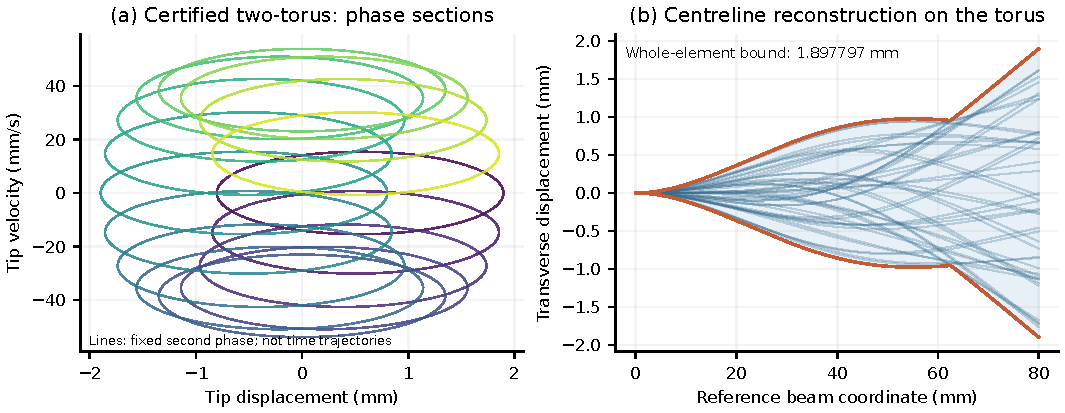
\includegraphics[width=\textwidth]{figures/fig_certified_torus_geometry.pdf}
\caption{The certified target torus in the same SI beam coordinates.
(a) Tip displacement and velocity along sampled sections with the second
phase fixed; these curves are not time trajectories.
(b) Sampled centerlines and a plotted phase envelope.
The separate whole-element Bernstein/Fourier certificate bounds every
centerline point on the corrected invariant torus by $1.897797$ mm.
Sampling illustrates the geometry; the analytic certificate supplies
the all-phase bound.}
\label{fig:certified-torus-geometry}
\end{figure*}

The additional low-noise fit connects the two certificates on one actual
learned Hamiltonian. Its nonzero derivative MSE is
$3.3866649\times10^{-17}$. The outward Gram lower bound
$6.0167\times10^{-8}$, together with the label and decoder error budgets,
gives a twist-error upper bound $2.81119\times10^{-4}$, smaller than
the target singular-value lower bound $3.03081\times10^{-4}$.
The fifth row of the table uses these same fitted coefficients. Thus
the nonzero-loss twist certificate and the finite-amplitude
KAM certificate concern the same fitted function; the latter additionally
uses the full analytic invariance residual, as required by the theorem.

The sixth row certifies the actual GC function obtained from four
independent COMSOL position--velocity trajectories by integral matching.
The fit uses state increments and feature integrals, without reconstructed
acceleration labels. Its exported cosine multiplier is
$a=1.022324882191665$; every exported quartic term is included in
the analytic verification, using the fitted coefficients without
re-estimation. The frequency in~\eqref{eq:certified-comsol-frequency}
admits the same conservative
$\gamma=9/1750$, so the global bounds and theorem constants above
remain unchanged. In this case the checked inverse averaged torsion
is below $94762$, within the required $10^5$ margin.

This result certifies one specified nonresonant torus in each Hamiltonian
at a useful physical amplitude. It does not attach a measured phase-space
volume to these individual tori. Positive-measure families near the elliptic
equilibrium follow from the separate normal-form argument above;
the finite-amplitude theorem and the energy-based safety theorem have
distinct hypotheses and conclusions.

\subsection{Positive-measure families around the certified tori}
\label{sec:certified-torus-families}

The nondegeneracy retained by the a posteriori iteration gives a further
conclusion at the same finite-amplitude motion.

\begin{corollary}[KAM stability of the certified finite-amplitude tori]
\label{cor:finite-torus-families}
Each of the six tori in Theorem~\ref{thm:beam-finite-tori}, and the
additional integral-COMSOL torus in
Section~\ref{sec:validated-integral-learning}, is accumulated by
positive-measure families of analytic Lagrangian invariant tori.
In analytic symplectic tubular coordinates $(\theta,I)$ centered on that
torus, their relative Lebesgue measure in
$\mathbb T^2\times\{|I|_\infty<r\}$ tends to one as $r\to0$.
This is an asymptotic statement about neighborhoods of the certified
millimetre-amplitude torus; it does not specify a numerical tube
thickness or a percentage in a preassigned experimental domain.
In particular, for any prescribed fraction $p<1$, a sufficiently thin
tube has relative invariant-torus measure greater than $p$. The present
statement is existential in the tube radius.
\end{corollary}

\begin{proof}
The inequalities controlling the inverse averaged torsion in the
Haro--Luque iteration are uniform at every step: see their
Eqs.~(5.65)--(5.67) and the summation in Section~5.3.
The strict margin used in~\eqref{eq:HL-evaluated-constants} therefore gives
\[
 \|\langle T_\infty\rangle^{-1}\|\leq2\times10^5.
\]
This is nondegeneracy of the final invariant object, not only of its
numerical approximation.

An analytic Lagrangian neighborhood chart $\Psi$ can be chosen with
$\Psi(\theta,0)=K_\infty(\theta)$ and first derivative
$D\Psi(\theta,0)=[L_\infty,N_\infty]$.
One construction starts with $K_\infty(\theta)+N_\infty(\theta)I$ and
uses the relative analytic Moser correction. The forms agree on the
zero section; the relative primitive and its correcting vector field
are $O(|I|^2)$, so the correction preserves this first jet.
In these coordinates invariance implies
\begin{equation}
 \begin{aligned}
 h\circ\Psi&=e+\varpi\cdot I+\tfrac12 I^\top A(\theta)I\\
 &\quad+O(|I|^3).
 \end{aligned}
 \label{eq:torus-tubular-hamiltonian}
\end{equation}
The automatic-reducibility identity of Haro--Luque Section~2.4 is
\[
 \begin{aligned}
 &DX_h(K_\infty)P-D_\varpi P\\
 &\qquad=P\begin{pmatrix}0&T_\infty\\0&0\end{pmatrix},
 \end{aligned}
\]
where $P=[L_\infty,N_\infty]$.
Comparing this with the linearized vector field of
\eqref{eq:torus-tubular-hamiltonian} gives $A=T_\infty$.
More generally, changing the symplectic normal frame to
$N_\infty+L_\infty S(\theta)$, with $S$ symmetric, changes this block
to $T_\infty-D_\varpi S$, whose average is the same.
Hence $\overline A=\langle A\rangle$ is nonsingular independently of
this choice of normal frame.

The quadratic normal form is justified without a formal-series
convergence assumption. Solve the matrix homological equation
$D_\varpi S=A-\overline A$ with zero average by
\[
 S_k=\frac{A_k}{2\pi i k\cdot\varpi}\quad(k\ne0),\qquad S_0=0.
\]
Equation~\eqref{eq:certified-dio} and analyticity make this series
convergent on every strictly smaller angle strip; the cohomological
bound established above controls it there.
The exact time-one Hamiltonian flow of
$\chi_2(\theta,I)=\tfrac12 I^\top S(\theta)I$ exists on a sufficiently
thin tube and fixes $I=0$. With the pullback convention
$L_{\chi}F=\{F,\chi\}$, it changes the quadratic coefficient to
$\overline A$ and leaves an analytic $O(|I|^3)$ remainder.
The resulting normal form satisfies the hypotheses of
\citet[Theorem~6, analytic case]{bounemoura2016torus}:
the frequency is nonresonant, the averaged quadratic form is
nonsingular, and the full remainder is analytic. That theorem gives
the claimed density-one families. Symplectic coordinate changes
preserve volume, and the constant factor relating the dimensionless
chart to SI canonical coordinates cancels in relative measure.
\end{proof}

This corollary establishes the local abundance of invariant tori around
the certified motion. Section~\ref{sec:measure-definition} defines their
relative measure on a specified phase-space domain. For the
integral-COMSOL fit, Appendix~\ref{app:measure-proof} supplements the local
result with an explicit symplectic chart, a complete analytic remainder
and a conservative quantitative bound on a fixed tube. The tube width
and the resulting measure bound are reported together to distinguish
this rigorous local estimate from the wider numerical sampling domain.

\subsection{A validated COMSOL state-to-KAM learning certificate}
\label{sec:validated-integral-learning}

We add a controlled identification experiment for the same complete
two-mode magnetic Hamiltonian. COMSOL independently integrates its four
state equations for $64$ initial conditions, with $17$ state observations
on each dimensionless interval $[0,T]$, $T\simeq0.04$.
This experiment is explicitly a two-mode modal ODE experiment; the
earlier $64$-DOF finite-element trajectories remain a separate validation.
Only positions and velocities enter the new training labels.
Neither acceleration reconstruction nor a solver tolerance is used as
an error certificate.

For each observed orbit, fit a degree-eight polynomial curve
$c_\ell:[0,T]\to\mathbb R^4$ to the observed states.
Its coefficients are frozen as exact dyadic rationals, with its constant
and linear coefficients corrected exactly so that both endpoints equal
the exported observations $z_\ell^-,z_\ell^+$.
This construction uses no evaluation of the physical acceleration.
Let $Lz=X_{h_2}(z)$ and let
$V(z)=[J\nabla F_0(z),\ldots,J\nabla F_{34}(z)]$
be the nonlinear feature field of the same learned family. Define
\begin{equation}
 \begin{aligned}
 D_\ell&=\frac1T\int_0^T V(c_\ell(\tau))\,d\tau,\\
 y_\ell&=\frac{z_\ell^+-z_\ell^-}{T}
          -\frac1T\int_0^T Lc_\ell(\tau)\,d\tau .
 \end{aligned}
 \label{eq:validated-integral-observations}
\end{equation}
The integral design and labels are therefore functions of the observed
state curves, not instantaneous force-balance labels.

\begin{proposition}[Integral loss, dynamic defect and coefficient error]
\label{prop:integral-transfer}
Let $\eta_\star=(s_4,0,\ldots,0)$ represent the declared full-cosine target,
and let $m$ be the number of observed curves. Put
\begin{equation}
 \begin{aligned}
 e_\ell&=\frac1T\int_0^T
       \bigl(\dot c_\ell-X_{h_\star}(c_\ell)\bigr)\,d\tau,\\
 G_I&=\frac1{4m}\sum_{\ell=1}^m D_\ell^\top D_\ell,\\
 r_I^2&=\frac1{4m}\sum_{\ell=1}^m
                   \|D_\ell\widehat\eta-y_\ell\|_2^2 .
 \end{aligned}
 \label{eq:integral-defect-gram}
\end{equation}
If $\lambda_{\min}(G_I)\geq\underline\lambda>0$ and
$(4m)^{-1}\sum_\ell\|e_\ell\|_2^2\leq\epsilon_I^2$, then
\begin{equation}
 \|\widehat\eta-\eta_\star\|_2
 \leq b_I:=\frac{r_I+\epsilon_I}{\sqrt{\underline\lambda}} .
 \label{eq:integral-coefficient-transfer}
\end{equation}
The curves need not be exact solutions of the physical differential
equation. Their explicitly verified dynamic defect supplies the required
error budget.
\end{proposition}

\begin{proof}
Exact endpoint matching and the fundamental theorem of calculus give
$y_\ell-D_\ell\eta_\star=e_\ell$.
The triangle inequality in the stacked, $1/(4m)$-normalized Euclidean
norm gives
$\|D(\widehat\eta-\eta_\star)\|_2/\sqrt{4m}\leq r_I+\epsilon_I$.
The Gram lower bound proves~\eqref{eq:integral-coefficient-transfer}.
\end{proof}

The defect is independently evaluated against the explicitly declared
physical target. Thus the proposition does not infer arbitrary unknown
model error from a small training loss. It certifies consistency with
this target using additional, verified physical information.

\paragraph{Validated integrals and numerical error.}
All polynomial feature integrals are evaluated by exact polynomial
integration with Arb ball coefficients. For $\vartheta=d^\top(c_\ell)_X$,
the magnetic feature uses the odd Taylor terms of
$\sin\vartheta-\vartheta$ through degree $19$, together with
\begin{equation}
 \begin{aligned}
 S_{19}(\vartheta)&=
 \sum_{\substack{3\leq j\leq19\\j\ {\rm odd}}}
       \frac{(-1)^{(j-1)/2}\vartheta^j}{j!},\\
 |\sin\vartheta-\vartheta-S_{19}(\vartheta)|
 &\leq\frac{R^{21}\cosh R}{21!},\quad |\vartheta|\leq R .
 \end{aligned}
 \label{eq:integral-sine-remainder}
\end{equation}
The computed maximum remainder is below $4.8752\times10^{-43}$.
The remainder is included in every affected feature integral and dynamic
defect; the certified function remains the complete cosine model.
The exact identity $y-D\eta_\star=e$ is also checked componentwise by
independent ball evaluations.

The interval Gram inverse is computed at $256$-bit precision.
Since the exact Gram matrix is real symmetric and positive semidefinite,
a validated inverse makes it positive definite and gives
$\underline\lambda=1/\|G_I^{-1}\|_\infty$.
Decoder rounding is retained when the real readout coefficients are
exported as a cosine multiplier and a quartic polynomial.
With $B=[q_\star/s_4\ U]$, this gives
\begin{equation}
 \begin{aligned}
 \|A_{\widehat\eta}-A_\star\|_2
 &\leq\sqrt{19}\bigl(\|B\|_2b_I+\delta_{\rm dec}\bigr),\\
 \|h_{\widehat\eta}-h_\star\|_r
 &\leq b_I B_F(r)+\delta_{h,\rm dec}(r).
 \end{aligned}
 \label{eq:integral-analytic-transfer}
\end{equation}
Here $\|B\|_2\leq\|B^\top B\|_\infty^{1/2}$ is verified from the
exported feature matrix; exact numerical orthogonality is unnecessary.
The analytic bound controls every derivative on a smaller polydisc by
Cauchy's estimate:
\[
 \begin{aligned}
 &\|\partial^\alpha(h_{\widehat\eta}-h_\star)\|_{r'}\\
 &\quad\leq\alpha!(r-r')^{-|\alpha|}
       \|h_{\widehat\eta}-h_\star\|_r .
 \end{aligned}
\]

\begin{table}[t]
\centering
\caption{Outward bounds for the independent COMSOL integral-learning
experiment. The MSE has a strictly positive certified lower bound.}
\label{tab:integral-certificate}
\begin{tabular}{lr}
\hline
Quantity & Certified bound\\
\hline
Training MSE & $[3.6030,3.6031]\,10^{-23}$\\
$r_I$ & $\leq6.0026\,10^{-12}$\\
$\epsilon_I$ & $\leq6.8835\,10^{-12}$\\
$\lambda_{\min}(G_I)$ & $\geq2.9302\,10^{-7}$\\
$\|\widehat\eta-\eta_\star\|_2$ & $\leq2.3805\,10^{-8}$\\
Twist error & $\leq1.0377\,10^{-7}$\\
$\sigma_{\min}(A_\star)$ & $\geq4.9032\,10^{-4}$\\
$\|h_{\widehat\eta}-h_\star\|_{0.3}$ & $\leq1.3310\,10^{-9}$\\
\hline
\end{tabular}
\end{table}

The target is unchanged. The singular-value lower bound in
Table~\ref{tab:integral-certificate} is a sharper bound for the same
two-by-two symmetric matrix:
$\sigma_{\min}(A_\star)\geq|\det A_\star|/\|A_\star\|_\infty$.
The previously reported, smaller lower bound remains valid.
The strict twist margin, fixed quadratic part and complete analytic
tail therefore give local positive-measure KAM families for this actual
fitted Hamiltonian by the normal-form argument above.

\paragraph{An independent bound on trajectory error.}
The observation curves deviate from every exported sample by at most
$5.2538\times10^{-14}$ and satisfy
\[
 \sup_\tau\|\dot c_\ell-X_{h_\star}(c_\ell)\|_2
 \leq1.0973\times10^{-8}.
\]
The linear modal field $L$ is skew symmetric in these balanced
coordinates. On the real box $|z|_\infty<0.3$, the nonlinear part has
Euclidean Lipschitz constant
\[
 \|d\|_2^2\frac{(0.3\|d\|_1)^2}{2}
 <0.002084<0.01 .
\]
For the exact physical solution $z_\ell$ with
$z_\ell(0)=c_\ell(0)$, variation of constants and Gronwall's inequality
therefore give
\[
 \begin{aligned}
 &\sup_{0\leq\tau\leq T}\|z_\ell(\tau)-c_\ell(\tau)\|_2\\
 &\quad\leq T e^{0.01T}
       \|\dot c_\ell-X_{h_\star}(c_\ell)\|_{\infty,2}\\
 &\quad<4.3907\times10^{-10}.
 \end{aligned}
\]
The verified curve bound $|c_\ell|_\infty<0.2000$ closes the
bootstrap inside the radius-$0.3$ box. This is an a posteriori bound
on the independently observed trajectories, not an interpretation of
COMSOL's requested time-stepping tolerances.

\paragraph{The same fitted function at millimetre amplitude.}
The frozen network has cosine multiplier
$a=0.9999996888354415$.
Its complete exported coefficients are also used in a separate,
$512$-bit a posteriori torus verification with the frequency in
Eqs.~\eqref{eq:certified-invariance}--\eqref{eq:certified-quadratic-frequency}
and the theorem constants of Theorem~\ref{thm:beam-finite-tori}.
The verified analytic invariance residual is at most
$2.7310\times10^{-77}$, the KAM smallness quotient is at most
$0.031724$, and the inverse averaged torsion is below $80526$.
The invariant torus lies within $2.0894\times10^{-41}$ of its exact
Fourier candidate. The tip-displacement witness is at least
$1.8977904$ mm, and the whole reconstructed centerline is bounded by
$1.8977962$ mm for every phase and all time.
Thus the nonzero integral-loss certificate and the finite-amplitude
KAM certificate concern exactly the same independently trained function.
The first proves coefficient, analytic and twist control; the second
checks the additional invariance-residual condition needed at the stated
finite amplitude.

The full-FE trajectory fit has an independent a posteriori torus
certificate, but its integral observation matrix yields a coefficient
bound above $0.025$ before accounting for continuous-quadrature and
model errors. This bound does not satisfy the coefficient condition
used here. The independently observed two-mode trajectories provide
the defect bounds needed for the complete integral-learning theorem;
model-reduction errors remain part of the separate full-FE evaluation.

\subsection{Phase-space measure of the invariant family}
\label{sec:measure-definition}

The positive-measure family established above motivates a domain-specific
measure of quasiperiodic initial states. A quantitative fraction requires
a specified volume measure and initial-state domain. Following the measure formulation of
\citet{biasco2018measure,chierchia2021measure}, let $U\subset\R^4$ be a
bounded domain of positive Liouville volume for the identified
two-degree-of-freedom Hamiltonian $h$, and
let $\mathcal K_h$ denote the union of its analytic Lagrangian invariant
tori carrying Diophantine quasiperiodic motion. Define
\begin{equation}
 f_{\rm KAM}(U)=\frac{\mu_L(U\cap\mathcal K_h)}{\mu_L(U)},
 \qquad \mu_L=\mathrm dX_1\,\mathrm dX_2\,\mathrm dY_1\,\mathrm dY_2.
 \label{eq:measure-fraction-definition}
\end{equation}
An explicitly certified subfamily provides a lower bound for this
fraction. The complement of that subfamily can contain other regular
motion; it is not thereby a chaotic set. The sampling confidence in a
learning bound such as that of \citet{chen2022} is a probability over
training data, whereas \eqref{eq:measure-fraction-definition} measures
initial states of one fixed fitted Hamiltonian.

For a symplectic chart $\Xi$ and an action box $D$, set
$U=\Xi(\mathbb T^2_{2\pi}\times D)$, where
$\mathbb T^2_{2\pi}=(\R/2\pi\mathbb Z)^2$. Then
$\mu_L(U)=(2\pi)^2\operatorname{area}(D)$.
The period-one angles used by the earlier torus certificate are changed
to radians together with the inverse action rescaling, preserving the
symplectic form. The constant volume factor in the SI canonical chart
also cancels from the relative fraction. The radius and location of $D$
must accompany every reported percentage.

Where the assumptions of Theorem~\ref{thm:full-fe-kam-lift} hold, the
invariant-family lift to the $64$-mode closed loop carries this
low-dimensional parameter measure forward. It does not turn it into a
positive fraction of the full $128$-dimensional Lebesgue volume.
Accordingly, the measure estimate in Appendix~\ref{app:measure-proof}
and the numerical sampling experiment in Section~\ref{sec:measure-numerical}
refer to the conservative low-mode Hamiltonian realized by the magnetic
feedback, with their respective domains specified separately.


The explicit constants of \citet{chierchia2021measure} yield a computable
local measure bound after construction of a symplectic tube and estimation
of the full analytic remainder. Appendix~\ref{app:measure-proof} gives that
construction for the integral-COMSOL Hamiltonian. Its sufficient estimates
certify an extremely thin transverse domain; the central motion remains
at millimetre amplitude, but the resulting width does not quantify an
experimentally resolvable initial-state tolerance. To examine a broader
range of amplitudes, Section~\ref{sec:measure-numerical} samples a prescribed
action domain and evaluates finite-time quasiperiodicity with independent
integration and averaging checks.


\section{Reproducible learning and independent COMSOL validation}
\label{sec:experiments}
\label{sec:unified-experiments}

All experiments in this section use the clamped-free beam, static-field
eigenvectors, complete magnetic cosine, and SI parameters defined above.
The two-mode learning problem and its higher-order validation models therefore
share the same mechanics. The reference energy is
\begin{equation}
 \begin{aligned}
 h_\star(X,Y)&=\frac12\sum_{j=1}^2\nu_j(X_j^2+Y_j^2)+g(d^TX),\\
 g(s)&=1-\cos s-\frac12s^2 .
 \end{aligned}
 \label{eq:unified-reference-energy}
\end{equation}
Here $\nu=(1,6.152117504)$ and
$d=(0.225670773,0.321798806)^T$; one dimensionless energy unit is
$6.0\times10^{-7}$ J and $\tau=11.417287283t$.
The tip displacement in metres is
$0.013506054X_1+0.005470926X_2$.
These mappings are used for every reported displacement, slope, and energy
error, including the independent COMSOL comparison.

\subsection{Finite-feature identification and matched controls}
\label{sec:unified-learning-protocol}
The CHNN uses $z_j=(X_j+\mathrm{i}Y_j)/\sqrt2$, conjugate polynomial
features, and a complex exponential feature for the full cosine.
Its real energy readout is
\begin{equation}
 h_\vartheta=h_2+a\,g(d^TX)+m_4(X,Y)^TUc,
 \label{eq:unified-feature-readout}
\end{equation}
where $m_4$ lists the 35 degree-four real monomials in $(X_1,X_2,Y_1,Y_2)$.
If $v_4$ is the coefficient vector of $-(d^TX)^4/24$, the 34 columns of
$U$ span its orthogonal complement. The feature $g/\|v_4\|_2$ and
these complementary quartics give 35 fitted real parameters, avoid
duplicating the leading cosine term, and retain the complete analytic
cosine tail. The target corresponds to $a=1,c=0$ and is therefore in the
feature class. The stored matrix $U$, rather than idealized exact
orthogonality, is used in the certificate computations.

We compare real (R) and complex (C) implementations, each with either the
fixed mechanical quadratic part (G) or a fitted general quadratic part (B).
Thus GR and GC have 35 fitted real parameters, whereas BR and BC have 45.
The two representations span the same real energy class, receive identical
data, and use the same regularizer expressed in common real feature coordinates.
Both implementations evaluate their respective real or complex features.
Because the representations are related by an invertible transformation,
this comparison tests their numerical implementation within a common
hypothesis class.

For each seed in $\{17,43,91\}$, we generate 12 conservative trajectories
of 4 s from the two-mode Python Galerkin model, sampled at 129 times.
Initial modal radii are drawn uniformly from
$[0.03,0.20]$ and $[0.03,0.16]$, with independent uniform phases.
The largest training tip slope is $0.0891$ rad.
Each component of the dimensionless vector-field label receives independent
uniform noise in $[-10^{-6},10^{-6}]$; states are noiseless.
Linear readout fitting minimizes derivative mean-square error with a
$10^{-14}$ quadratic regularizer.
Eight independent trajectories, generated with a separate seed and
integrated for 16 s at 1601 output times, are held out in full.
The reference solver is DOP853 with relative and absolute tolerances
$2\times10^{-10}$ and $2\times10^{-12}$.
Tightening both tolerances by a factor of 100 changes the tip of the first
held-out trajectory by at most $1.92\times10^{-8}$ mm.

\begin{table*}[t]
\centering
\caption{Conservative held-out errors, mean $\pm$ sample standard deviation
over three training seeds. Each seed is evaluated on all eight independent
16 s trajectories. These are errors within the declared simulated model.}
\label{tab:unified-learning}
\small
\begin{tabular}{lccc}
\hline
Model & Tip RMSE (mm) & Slope RMSE (mrad) & Energy RMSE (nJ)\\
\hline
BR & $(2.28\!\pm\!0.75)10^{-5}$ & $(5.80\!\pm\!1.20)10^{-4}$ & $(3.21\!\pm\!0.51)10^{-6}$\\
BC & $(2.28\!\pm\!0.75)10^{-5}$ & $(5.80\!\pm\!1.20)10^{-4}$ & $(3.21\!\pm\!0.51)10^{-6}$\\
GR & $(1.20\!\pm\!0.71)10^{-5}$ & $(3.90\!\pm\!1.63)10^{-4}$ & $(3.14\!\pm\!0.71)10^{-6}$\\
GC & $(1.20\!\pm\!0.71)10^{-5}$ & $(3.90\!\pm\!1.63)10^{-4}$ & $(3.14\!\pm\!0.71)10^{-6}$\\
\hline
\end{tabular}
\end{table*}

Table~\ref{tab:unified-learning} and Fig.~\ref{fig:unified-learning}
show the benefit of fixing the known quadratic mechanics in this
experiment, while matched real and complex fits agree to numerical
precision. GC identifies $a=1.00326\pm0.00154$ with nonzero training
residuals. The energy error evaluates the true energy along the predicted
and reference states; it is not an energy-conservation surrogate for
trajectory accuracy. The small fitting errors reflect exact representation,
accurate synthetic derivatives, and deliberately controlled label noise.
They do not establish corresponding physical measurement accuracy.

\begin{figure*}[t]
\centering
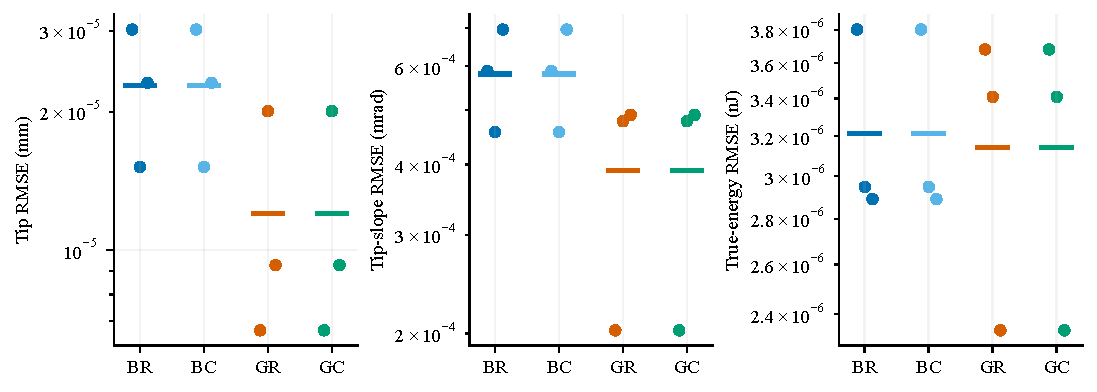
\includegraphics[width=\textwidth]{figures/fig_unified_learning.pdf}
\caption{Identical full-cosine beam data and real parameter budgets for the
four learning controls. Points are individual seeds and horizontal marks
are means. The quadratic mechanics prior changes the result; the matched
real/complex representation changes it only at numerical precision.}
\label{fig:unified-learning}
\end{figure*}

We also continue one independent initial condition for 200 s, or
363 first-mode linear periods, using the three primary GC fits.
The seed-level tip RMSE ranges from $1.38\times10^{-4}$ to
$4.03\times10^{-4}$ mm; the largest modal phase error is
$4.19\times10^{-4}$ rad. The relative drift of each learned model's own
energy remains below $5.11\times10^{-9}$ with conservative integration
at relative and absolute tolerances $2\times10^{-11}$ and $2\times10^{-13}$.
Figure~\ref{fig:unified-long} shows its Poincar\'e section, phase error,
and numerical energy drift. These finite-time diagnostics assess the
fitted dynamics; they do not estimate the measure of KAM tori or replace
the analytic certificate.

\begin{figure*}[t]
\centering
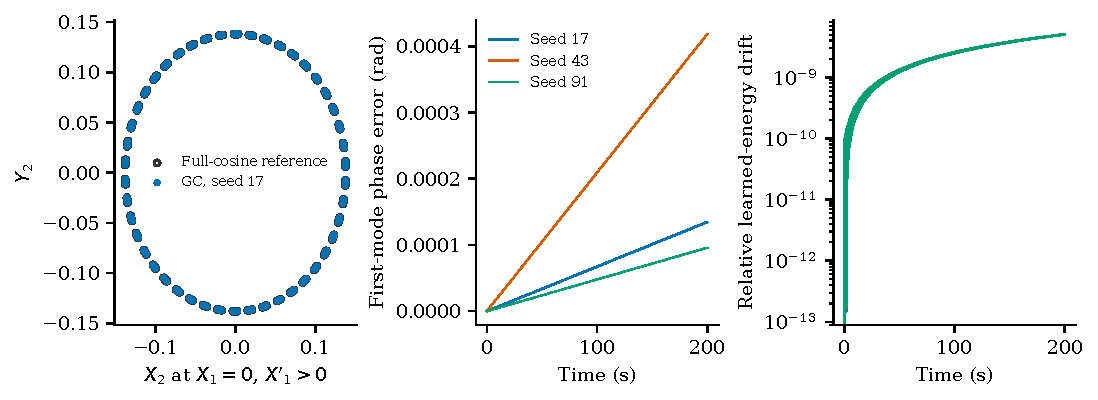
\includegraphics[width=\textwidth]{figures/fig_conservative_long_horizon.pdf}
\caption{Conservative 200 s continuation of an independent initial state.
Left: 364 upward crossings of $X_1=0$ for the reference and GC17.
Middle: unwrapped first-mode phase errors of the three learned energies.
Right: each learned energy's relative integration drift. All ports are
closed for these conservative diagnostics.}
\label{fig:unified-long}
\end{figure*}

\subsection{A nonzero-loss certificate for the fitted magnetic energy}
\label{sec:unified-loss-certificate}
The feature derivatives make the empirical Gram matrix and the complete
quartic Taylor map computable. We repeat the same three fits at noise
amplitudes $10^{-8}$ and $10^{-9}$, in addition to the $10^{-6}$
experiments. Outward-rounded interval calculations enclose the derivatives
of the analytic sine feature at the stored states, the Gram inverse
residual, the observed loss, clean-label rounding, and the conversion from
readout weights to the exported energy coefficients.
The degree-17 sine series is enclosed with its degree-19 remainder.

For the target magnetic quartic,
$A_{jj}=-d_j^4/8$ and $A_{12}=-d_1^2d_2^2/4$.
This twist is indefinite and nonsingular. Exact rational arithmetic on the
stored dyadic $d$ gives the conservative lower bound
$\sigma_{\min}(A_\star)>3.03081\times10^{-4}$.
If $G$ is the derivative Gram matrix, $B$ the quartic coefficient map,
$\ell$ the noisy derivative MSE, and $\eta_{\rm eff}$ the enclosed noise
and arithmetic budget, the verified sufficient inequality is
\begin{equation}
 \sqrt{19}\left(
 \|B\|_2\frac{\sqrt{\ell}+\eta_{\rm eff}}
                  {\sqrt{\lambda_{\min}(G)}}+\delta_{\rm dec}
 \right)<\sigma_{\min}(A_\star),
 \label{eq:unified-verified-twist}
\end{equation}
where $\delta_{\rm dec}$ encloses readout decoding roundoff.
At $\eta=10^{-8}$, Table~\ref{tab:unified-gram} verifies this inequality
with strictly positive losses for all seeds. Thus the data-dependent
error bound itself transfers nondegeneracy to the actual learned
Hamiltonians. The local KAM conclusions additionally use the nonresonance
and analytic normal-form hypotheses proved for this same model.
This table alone does not certify a finite experimental oscillation radius.
For the primary $10^{-6}$ fits, this sufficient error bound is too loose;
their directly computed twist singular values are nevertheless between
$5.78\times10^{-4}$ and $5.93\times10^{-4}$.

\begin{table*}[t]
\centering
\caption{Enclosed loss-to-twist checks at noise amplitude $10^{-8}$.
All twist-error upper bounds are below $3.03081\times10^{-4}$.}
\label{tab:unified-gram}
\small
\begin{tabular}{rccc}
\hline
Seed & Noisy MSE & Gram eigenvalue lower bound & Twist-error upper bound\\
\hline
17 & $3.387\times10^{-17}$ & $6.0167\times10^{-8}$ & $2.8112\times10^{-4}$\\
43 & $3.275\times10^{-17}$ & $2.2734\times10^{-7}$ & $1.4374\times10^{-4}$\\
91 & $3.283\times10^{-17}$ & $2.0968\times10^{-7}$ & $1.4973\times10^{-4}$\\
\hline
\end{tabular}
\end{table*}

\subsection{Learning dissipation and opening the magnetic input port}
The imaginary readout is the nonnegative Rayleigh potential
$\mathcal D_\gamma(v)=\gamma\sum_jv_j^2/(2\nu_j)$, with $v=h_{\vartheta,Y}$.
For each seed, eight additional damped, unforced 5 s trajectories provide
noisy derivative labels. Nonnegative least squares fits the single
$\gamma$ using the already fitted conservative gradient. In particular,
the decoder retains the learned momentum-dependent quartics:
\begin{equation}
 \begin{aligned}
 X'&=h_{\vartheta,Y},\\
 Y'&=-h_{\vartheta,X}-\gamma\operatorname{diag}(\nu^{-1})h_{\vartheta,Y}\\
   &\quad+u\,d\cos(d^TX).
 \end{aligned}
 \label{eq:unified-learned-port}
\end{equation}
The fitted dimensional mass-drag coefficients are
$0.555585710$, $0.555587102$, and $0.555584024$ s$^{-1}$, compared with
$0.555585237$ s$^{-1}$ for the generator.
On six independent driven trajectories with amplitudes 4--8 mT and
frequency ratios $0.65$--$1.20$ relative to the biased first frequency,
the three seed-level tip RMSEs are
$8.83\times10^{-5}$, $1.37\times10^{-4}$, and
$6.40\times10^{-5}$ mm. Closing the learned drag port increases the
tip RMSE to approximately $3.01$ mm.
The integrated work balance is
\begin{equation}
 \begin{aligned}
 h_\vartheta(\tau)-h_\vartheta(0)
 &=\int_0^\tau u\cos(d^TX)d^Th_{\vartheta,Y}\,ds\\
 &\quad-\int_0^\tau\gamma\sum_jh_{\vartheta,Y_j}^2/\nu_j\,ds.
 \end{aligned}
\end{equation}
Its largest numerical residual across these cases is
$4.41\times10^{-17}$ J.
These driven tests assess the port model, rather than autonomous KAM
persistence. Some stress cases exceed the channel clearance and are
free-motion continuations; safe operating trajectories are evaluated
separately with the physical energy bound and input governor.

\begin{figure*}[t]
\centering
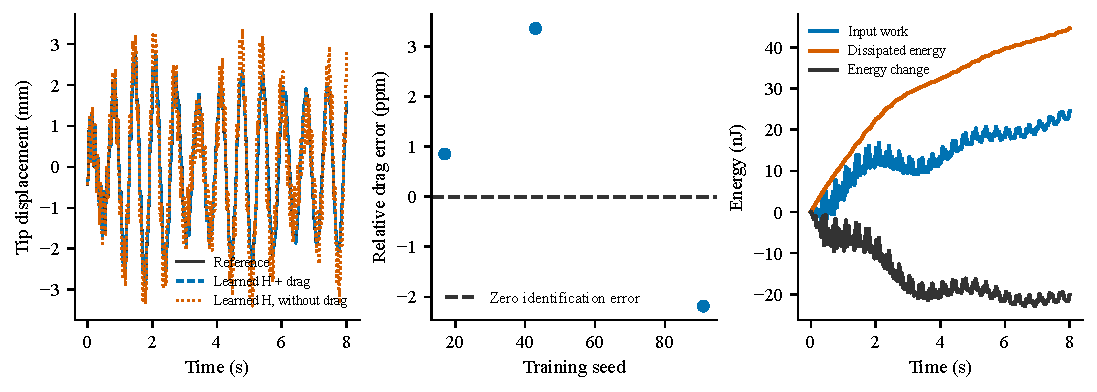
\includegraphics[width=\textwidth]{figures/fig_unified_ports.pdf}
\caption{The same learned conservative energy with an identified
nonnegative drag readout and magnetic input port. Left: an independent
driven trajectory and the drag ablation. Middle: signed relative errors
in the drag coefficient. Right: supplied work, dissipated energy, and
stored-energy change for that trajectory.}
\label{fig:unified-ports}
\end{figure*}

\subsection{Independent COMSOL assembly and nonlinear time integration}
\label{sec:unified-comsol}
COMSOL Multiphysics 6.3 independently assembles the same 32-element
clamped-free beam and solves its nonlinear magnetic-tip response.
The relative Frobenius differences between the exported and Python
consistent-mass matrices are $7.75\times10^{-15}$ for mass and
$3.05\times10^{-14}$ for bending stiffness.
The nonlinear held-out COMSOL trajectory starts from rest, uses the
same mass drag, and applies
\begin{equation}
 B_y(t)=0.006\,[1-\exp(-(t/0.25)^2)]\sin(\Omega t)\quad\mathrm{T}
\end{equation}
with $\Omega=9.4449490256$ rad/s for 8 s, relative tolerance $10^{-7}$,
and 2001 output samples.
The exported nodal displacement, rotation, velocity, and angular velocity
are evaluated directly, with no fitting to this driven trajectory.
Its peak tip displacement is $3.09032$ mm.
A separate COMSOL solve with relative tolerance $10^{-8}$ changes the
tip by $4.59\times10^{-5}$ mm RMSE and reduces its discrepancy against
the full Python FE solution to $1.03\times10^{-5}$ mm RMSE. The original
held-out dataset is used for the primary comparison below.

\begin{table*}[t]
\centering
\caption{Independent nonlinear COMSOL trajectory comparison. Modal models
use the common static-field chart. GC includes learned drag; its range
covers the three primary training seeds.}
\label{tab:unified-comsol}
\small
\begin{tabular}{lcc}
\hline
Predictor & Tip RMSE (mm) & Maximum tip error (mm)\\
\hline
2-mode exact cosine & $0.0156168$ & $0.0226548$\\
4-mode exact cosine & $0.00407422$ & $0.00592596$\\
8-mode exact cosine & $0.00102484$ & $0.00152782$\\
64-mode Python FE & $0.00005614$ & $0.00011835$\\
2-mode learned GC & $0.0156171$--$0.0156177$ & $0.0226545$--$0.0226549$\\
\hline
\end{tabular}
\end{table*}

The nested modal comparison in Table~\ref{tab:unified-comsol} separates
reduction error from learning error. Against the exact two-mode response,
GC contributes only $1.81\times10^{-6}$--$3.48\times10^{-6}$ mm tip RMSE
for this input. Against COMSOL, both have approximately $0.0156$ mm RMSE.
The two-mode maximum slope discrepancy is $3.69$ mrad; its true stored-energy
RMSE is $0.132$ nJ. These discrepancies decrease with modal enrichment.
Figure~\ref{fig:unified-comsol} shows the response and both error scales.
The primary training data were generated by the two-mode Python
Galerkin model; the COMSOL time history is an independent held-out
validation dataset. Neither dataset is a physical hardware measurement.

\begin{figure*}[t]
\centering
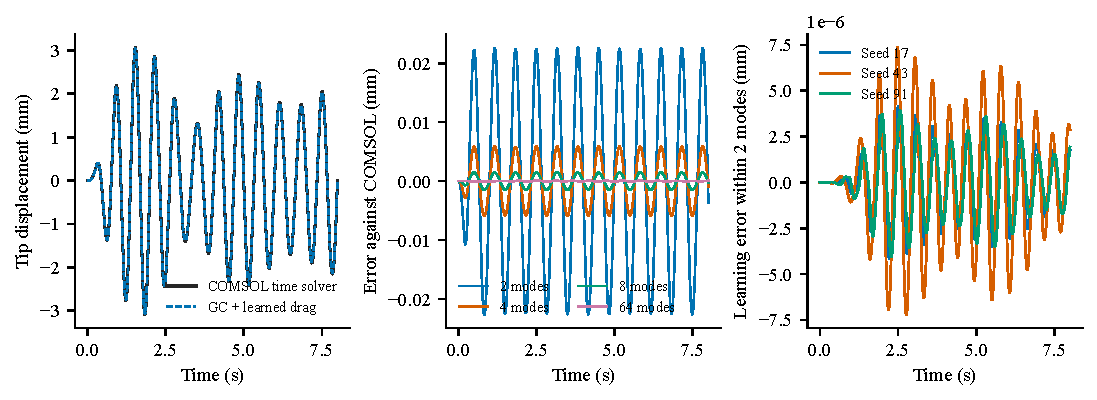
\includegraphics[width=\textwidth]{figures/fig_comsol_heldout.pdf}
\caption{Independent nonlinear COMSOL time integration. Left: COMSOL and
the learned two-mode GC response with learned drag. Middle: errors of
the nested exact-cosine modal models against COMSOL. Right: the additional
GC identification error within the two-mode model. Reduction error is
the larger contribution in this validation.}
\label{fig:unified-comsol}
\end{figure*}

\subsection{COMSOL-derived training data and an independent integral check}
\label{sec:comsol-identification}
We generate a separate conservative COMSOL dataset comprising four 4 s
training trajectories and two independent 8 s test trajectories, sampled
every 0.004 s. Initial displacements and velocities excite both retained
modes. The remaining 62 modes receive the static response to the nonlinear
magnetic residual and its compatible first time derivative; all 64 modes
remain active during integration. This initial tail condensation is not
assumed to be an exact nonlinear invariant manifold. Native solver-vector
checks confirm that the exported initial displacement and velocity are
correct; small changes introduced by consistent initialization are handled
by starting each predictor from the actual exported state.

The derivative-label construction requires care. At the stored output
times, the exported second time derivatives differentiate a time
interpolant and show a substantial lag relative to the velocity evolution.
For example, the first trajectory has a dimensionless modal equation-residual
RMS of $4.58\times10^{-2}$ when those derivatives are used directly.
We therefore reconstruct instantaneous acceleration from the exported
COMSOL mass and stiffness matrices:
\begin{equation}
 \ddot q=M_{\rm C}^{-1}
 \left[-K_{\rm C}q-\mu B_0\sin(\theta_{\rm tip})e_\theta\right].
 \label{eq:comsol-force-labels}
\end{equation}
The training states and velocities therefore come from the COMSOL
time solver, while the acceleration labels use known physical force
balance. This is surrogate identification for the declared mechanical
model with force-balance labels. The unresolved-mode force is included:
its largest component is $3.36\times10^{-9}$ in dimensionless
units for the checked training trajectory, and the remaining reconstructed
equation-residual RMS is $1.81\times10^{-10}$.

These COMSOL-based models are fitted separately from the primary
Python-trained GC models. Three seeds vary the
additional componentwise label noise, bounded by $10^{-6}$, while using
the same four COMSOL trajectories. The real/complex and prior/no-prior
controls use the same parameter budgets as before.

An independent check uses only the COMSOL displacement and velocity
samples. A nine-point closed Newton--Cotes rule integrates the vector-field
features on nonoverlapping 0.032 s windows, and the observed state
increments provide the regression targets. No acceleration or
force-balance label enters this integral fit.
With the initial solver settings (relative tolerance $10^{-6}$ and
scaled absolute tolerance $10^{-5}$), the integral residual is too large
to resolve the weak magnetic correction reliably: on the first trajectory,
its RMS is 2.16 times the nonlinear magnetic signal. An unconstrained
35-feature integral fit then yields $a=1.437$, illustrating that a good
fit to a numerically dispersed trajectory need not recover the physical
magnetic coefficient. A stricter COMSOL solve, with relative tolerance
$10^{-8}$ and scaled absolute tolerance $10^{-7}$, reduces that ratio
to 0.112 on the same trajectory. This independent data-quality check
resolves time-integration error that the force-balance loss alone
does not detect.

All six trajectories were then integrated with these stricter
tolerances. The refined runs use
generalized-alpha integration with high-frequency spectral radius zero
and backward-Euler consistent initialization. The four refined training
trajectories provide 500 integral windows, or 2000 scalar equations, for
the 35 real readout parameters. The resulting GC model has
$a=1.0223248822$ and a nonzero averaged-derivative integral RMS residual
of $4.0524\times10^{-7}$. The corresponding residuals of the quadratic
prior alone and the physical full-cosine target are
$3.9099\times10^{-6}$ and $6.6454\times10^{-7}$; the nonlinear magnetic
signal RMS is $3.6601\times10^{-6}$.
The fitted quartic twist has minimum singular value
$5.1166\times10^{-4}$. The conservative weights were frozen before
evaluating the two independent refined test trajectories.

\begin{table*}[t]
\centering
\caption{Independent refined COMSOL tests of the GC model identified
only from displacement and velocity increments. Predictions start from
each actual exported initial state. Energy errors use the physical
stored-energy function evaluated along the learned trajectory.}
\label{tab:comsol-integral-tests}
\small
\begin{tabular}{lccccc}
\hline
Test & Tip RMSE & Max. tip error & Slope RMSE & Energy RMSE & Exact 2-mode\\
 & ($\mu$m) & ($\mu$m) & (mrad) & (nJ) & tip RMSE ($\mu$m)\\
\hline
1 & $0.14836$ & $0.39240$ & $0.008677$ & $0.0002067$ & $0.24172$\\
2 & $0.05140$ & $0.17435$ & $0.002411$ & $0.0002253$ & $0.27459$\\
\hline
\end{tabular}
\end{table*}

Table~\ref{tab:comsol-integral-tests} and
Figure~\ref{fig:comsol-integral-tests} report the held-out errors.
The integral fit partly absorbs the remaining time-solver dispersion:
its agreement with COMSOL is better than that of the exact closed
two-mode target, despite a $2.23\%$ error in the cosine multiplier.
These errors quantify identification against simulated observations.
The requested solver tolerances do not supply a rigorous defect budget
for applying the loss-based certificate to these integral residuals.
The separate two-mode short-trajectory experiment in
Section~\ref{sec:validated-integral-learning} supplies a verified integral
defect budget and the corresponding loss-based certificate for its own
frozen fitted function.

\begin{figure*}[t]
\centering
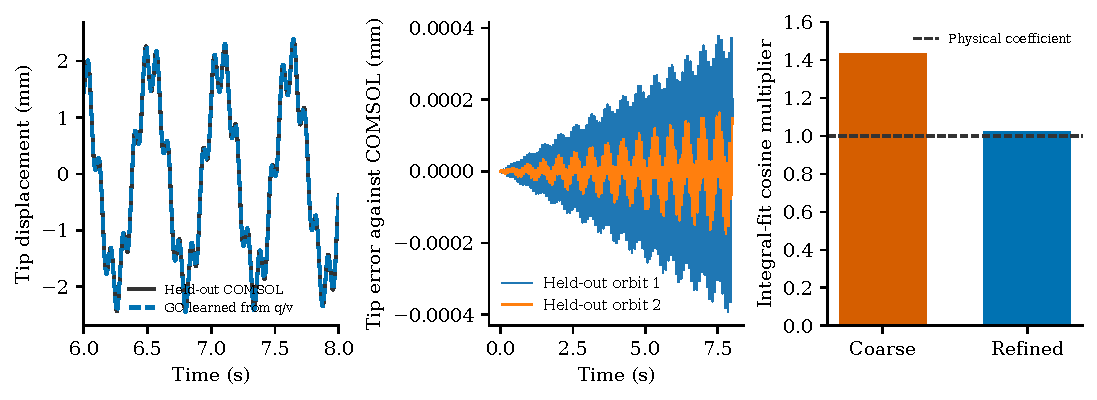
\includegraphics[width=\textwidth]{figures/fig_comsol_qv_identification_refined.pdf}
\caption{Identification using full-FE COMSOL displacement and velocity
outputs only. Left: independent test response. Middle: prediction errors
for both held-out trajectories. Right: the fitted cosine multiplier
under the two declared COMSOL tolerance settings; the physical value is
one. The refined coefficients are held fixed during the subsequent evaluations.}
\label{fig:comsol-integral-tests}
\end{figure*}

For comparison, the separately fitted models using the known-force
labels in~\eqref{eq:comsol-force-labels} recover $a=1.0000690$ without
added label noise. With the three added-noise seeds, the prior-informed
GC models give $0.25347$--$0.25940\,\mu$m pooled tip RMSE against the
same refined COMSOL tests; their additional error relative to the
closed two-mode trajectories is $0.00364$--$0.00771\,\mu$m.
Matched real and complex features again give coincident results to
numerical precision.

Finally, the position--velocity fit is used in the
independent a posteriori proof of
Section~\ref{sec:unified-aposteriori}. Its complete cosine and all fitted
quartic coefficients yield an analytic residual below
$2.7330\times10^{-77}$ and a theorem smallness quantity below $0.031746$.
The resulting exact invariant torus has a tip-displacement witness above
$1.8977374$ mm and a whole-centreline upper bound below $1.8977433$ mm.
This certificate concerns the actual fitted Hamiltonian and does not
require its coefficients to equal the physical target.
The same frozen conservative readout is paired with a nonnegative
drag coefficient refitted on the existing Python damped-beam trajectories,
$\gamma=0.0486617702$ for seed 17. Its independent driven COMSOL tip
RMSE is $0.015622$ mm. Section~\ref{sec:unifiedlearnedcontrol} then uses
this same energy, full gradient and Hessian, and drag readout to generate
the magnetic tracking input.

\subsection{Finite-time fraction in an operating action annulus}
\label{sec:measure-numerical}
We examine the phase-space fraction defined in
Section~\ref{sec:measure-definition} on a domain spanning millimetre-scale
oscillations. The Hamiltonian is identified from the two-mode COMSOL
position--velocity data in Section~\ref{sec:validated-integral-learning}.
In its canonical coordinates, set
\begin{equation}
 \begin{aligned}
 I_j&=\tfrac12(X_j^2+Y_j^2),\quad j=1,2,\\
 \phi_j&=\operatorname{atan2}(-Y_j,X_j).
 \end{aligned}
 \label{eq:measure-operating-actions}
\end{equation}
and prescribe, before classifying any orbit,
\begin{equation}
 \mathcal D_{\mathrm{op}}=[0.0032,0.0072]^2\times\mathbb T^2_{2\pi}.
 \label{eq:measure-operating-domain}
\end{equation}
Both harmonic modal radii therefore lie in $[0.08,0.12]$, surrounding the
radius $0.1$ of the previously certified $1.898\,\mathrm{mm}$ torus.
The corresponding harmonic tip envelope
$|\ell_1|\sqrt{2I_1}+|\ell_2|\sqrt{2I_2}$ ranges from
$1.518$ to $2.277\,\mathrm{mm}$.
The canonical polar Jacobian has absolute determinant one, so independent
uniform actions and phases sample normalized four-dimensional Liouville volume:
\begin{equation}
 \mu_L(\mathcal D_{\mathrm{op}})
   =(2\pi)^2(0.004)^2=6.3165468\times10^{-4}.
 \label{eq:measure-operating-volume}
\end{equation}
We draw $N=1024$ independent points with PCG64 seed $20261002$; the domain,
initial points, observables, and decision thresholds are specified before
classification. These points are independent of the training observations and the
certified-torus phase grid.

Following weighted Birkhoff averaging~\citep{das2017quasiperiodicity,duignan2023flows},
we compare consecutive windows using the smooth bump
$b(s)=\exp[-1/(s(1-s))]$ for $0<s<1$, with $b=0$ otherwise.
The normalized weighted mean is
\begin{equation}
 W_T(F;z)=\frac{\int_0^T b(t/T)F(\Phi_h^t z)\,dt}
                      {T\int_0^1 b(s)\,ds},
 \label{eq:measure-weighted-average}
\end{equation}
where $\Phi_h^t$ denotes the flow of the fitted Hamiltonian $h$.
The computations use normalized sampled sums of this weight; integration
and quadrature refinements are reported below.
Eight observables are used:
$X_j/0.1$, $Y_j/0.1$, $I_j/0.005$, $X_1X_2/0.01$, and $Y_1Y_2/0.01$.
We also average the polar angular velocities
\begin{equation}
 \dot\phi_j=
 \frac{X_j\partial_{X_j}h+
       Y_j\partial_{Y_j}h}{X_j^2+Y_j^2}.
 \label{eq:measure-angular-frequency}
\end{equation}
For each $T\in\{512,1024,2048,4096\}$, let $e_F(T)$ be the largest
absolute difference of the eight weighted means on $[0,T]$ and $[T,2T]$,
and let $e_\omega(T)$ be the largest relative difference of the two
weighted frequencies. A candidate passes the principal test when
$e_F,e_\omega\le10^{-8}$ at both $T=2048$ and $4096$.
It must also keep both sampled actions above $3.2\times10^{-4}$, have sampled
relative energy drift below $10^{-8}$, and satisfy the finite-order screen
\begin{equation}
 \min_{\substack{0<|k|_1\le64\\k\in\mathbb Z^2\ {\rm primitive}}}
 \frac{|k\cdot\overline\omega|}{|k|_1\|\overline\omega\|_\infty}
 >10^{-7},
 \label{eq:measure-finite-resonance-screen}
\end{equation}
where $\overline\omega$ uses the two longest consecutive windows.
The total simulated time is $8192/\omega_0=717.508\,\mathrm{s}$.
Full cosine and momentum-dependent quartic terms are retained.

Step refinement resolves integration error in the diagnostics. Fixed-step eighth-order DOP853
at $\Delta\tau=1/16$ produces relative energy drift up to $3.94\times10^{-7}$ and
fails the numerical validity test. At $\Delta\tau=1/32$, all points pass the principal
eight-digit criterion and the energy test, but the consecutive-window
averages fail the ten-digit criterion.
Refining all $1024$ trajectories to $\Delta\tau=1/64$, with the same initial
points and thresholds, resolves the ten-digit criterion.
The largest relative energy drift then falls to $6.11\times10^{-12}$;
$e_F(4096)\le4.49\times10^{-12}$ and
$e_\omega(4096)\le3.63\times10^{-14}$.
Halving the step again for the preselected first $64$ points changes no
six-, eight-, or ten-digit labels, with maximum relative frequency change
$2.40\times10^{-14}$. Halving the averaging output interval on identical
saved trajectories changes the weighted means by at most $3.82\times10^{-14}$.
An independent adaptive solver, phase points from the certified torus's
Fourier approximation, an exactly
resonant oscillator, and regular/chaotic two-wave examples provide additional
checks. In particular, the resonant oscillator passes the averaging test but
is rejected by~\eqref{eq:measure-finite-resonance-screen}.

The refined ensemble gives $1024/1024$ candidates at each of the six-, eight-,
and ten-digit thresholds. For the specified finite-time classifier $C$,
\begin{equation}
 \begin{aligned}
 \widehat p_C&=\frac1{1024}\sum_{i=1}^{1024}\mathbf1_C(z_i)=1,\\
 \mathrm{CI}_{95\%}(p_C)&=[0.996404,1].
 \end{aligned}
 \label{eq:measure-empirical-fraction}
\end{equation}
using the two-sided exact Clopper--Pearson interval.
The smallest normalized finite-order detuning is $2.113\times10^{-4}$;
the largest sampled tip displacement is $2.269\,\mathrm{mm}$.
Figure~\ref{fig:measure-finite-time} shows the fixed-domain sample and the
integration and threshold checks.
This interval quantifies only random initial-condition sampling for $C$.
It does not bound classification error, unresolved high-order resonance,
sticky chaos, or physical model error. Thus~\eqref{eq:measure-empirical-fraction}
is an empirical finite-time candidate fraction in the operating domain.
Its $99.6404\%$ lower confidence endpoint concerns the classifier probability,
whereas Appendix~\ref{app:measure-proof} establishes a rigorous KAM-volume
bound on a separate, narrower analytic domain.

\begin{figure*}[t]
 \centering
 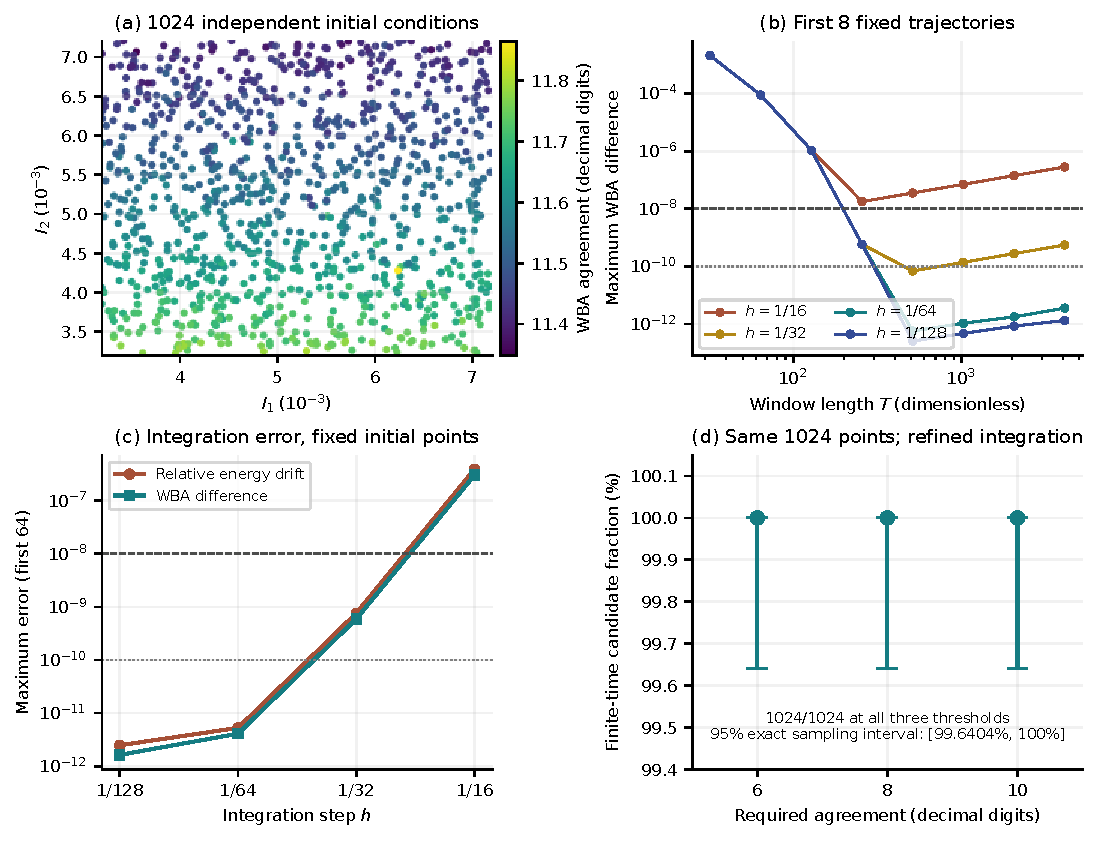
\includegraphics[width=0.95\textwidth]{figures/finite_time_quasiperiodicity.pdf}
 \caption{Finite-time quasiperiodicity diagnostics for the fitted
 Hamiltonian. (a) Uniform action sampling; angles are independently uniform.
 (b) Consecutive-window agreement on the first eight fixed trajectories;
 the long-window floor reflects integration error and roundoff.
 (c) Step refinement on the first $64$ fixed initial points identifies
 the coarse integration error.
 (d) Candidate fractions and exact sampling intervals at three thresholds,
 using the same $1024$ points with refined integration.
 Candidate status describes finite-time agreement of the specified observables.}
 \label{fig:measure-finite-time}
\end{figure*}

\subsection{State-only identification beyond the nominal hypothesis class}
\label{sec:robustness-newphysics}
The nominal full-cosine experiment places its target inside the chosen
feature class. We additionally test unknown material and magnetic
parameters, state noise, and two omitted physical effects. All training
observations in this experiment are generated by the full $32$-element,
$64$-DOF Python FE plant; the predictors retain the same four nominal
static-field modes. Let $e=E/E_{\rm ref}$ and $m=\mu/\mu_{\rm ref}$.
The local applied field is
\begin{equation}
 B_x=B_0-G(x-L),\qquad B_y=B_y(t)+Gy.
 \label{eq:robust-gradientfield}
\end{equation}
The field is curl-free and divergence-free. Under the declared
linear-beam kinematics, $x_{\rm tip}=L$, so its additional potential is
$-\mu G w(L)\sin\vartheta$. It supplies both the transverse tip force
$\mu G\sin\vartheta$ and the corresponding moment
$\mu G w(L)\cos\vartheta$. The axial force $-\mu G\cos\vartheta$ is
balanced by the axial constraint reaction and does no virtual work in
this specialization. We also add the still-fluid Morison drag density
$-c_2|w_t|w_t$, with dissipation potential
$c_2\int_0^L|w_t|^3ds/3$.

In the fixed dimensionless chart, the conservative energy is
\begin{align}
 h={}&\tfrac12Y^{\mathsf T}\operatorname{diag}(\nu)Y
 +\tfrac e2 X^{\mathsf T}A_{\rm el}X
 +m(1-\cos\vartheta)\nonumber\\
 &-g\frac{G_{\rm ref}}{B_0}(\ell^{\mathsf T}X)\sin\vartheta,
 \qquad \vartheta=d^{\mathsf T}X,
 \label{eq:robust-energy}
\end{align}
where $A_{\rm el}=\operatorname{diag}(\nu)-dd^{\mathsf T}$,
$G_{\rm ref}=0.5$ T/m, and $g=mG/G_{\rm ref}$.
The five fitted readouts are $(e,m,g,\alpha/\alpha_{\rm ref},
c_2/c_{2,\rm ref})$, with $c_{2,\rm ref}=0.02$ kg/m$^2$.
The elastic and magnetic strengths and both dissipative coefficients are
constrained to be nonnegative; the gradient may have either sign.
The kinetic metric is known. Complex features evaluate the polynomial
and exponential terms through $z=(X+iY)/\sqrt2$ and its conjugate.

Each of three parameter settings provides six independent $3$ s training
trajectories and three $4$ s tests with different initial conditions and
multisine inputs. The two changed settings use respectively
$(e,m,\alpha/\alpha_{\rm ref},G,c_2)
=(0.85,1.20,1.40,0.5,0.02)$ and
$(1.20,0.85,0.70,-0.4,0.012)$ in SI units where dimensional.
The first four modes are excited, and the remaining initial coordinates
are statically condensed with zero initial velocity. This construction
does not assume an invariant modal manifold. Samples are separated by
$1$ ms. On overlapping $32$ ms windows, multiplication by
$\psi=\sin^4(\pi s)$ and integration by parts gives
\begin{equation}
 -\int\psi'Y\,d\tau=\int\psi F_\theta(X,Y,u)\,d\tau.
 \label{eq:robust-weakfit}
\end{equation}
The endpoints of $\psi$ vanish. Fitting therefore uses only positions,
velocities and the applied field; neither accelerations nor reconstructed
force-balance labels enter the regression.

We compare the expanded CHNN with a three-readout model that re-identifies
elasticity, magnetic strength and linear drag but omits the gradient and
quadratic drag. A further control freely learns the ten entries of the
symmetric quadratic potential while retaining the analytic magnetic
features and dissipative heads, giving fourteen readouts. Thus every
comparison uses four modes. Matched real and complex realizations agree
in effective coefficients to $1.31\times10^{-11}$ or better. The experiment
does not attribute an accuracy advantage to complex arithmetic.

\begin{table}[t]
\caption{Mean tip RMSE over three independent full-FE tests in $\mu$m.
The noisy entries average three independent training-noise seeds; the
clean fit is counted once. The last control has a freely learned
quadratic potential.}
\label{tab:robustness-state-noise}
\centering\small
\begin{tabular}{llrrr}
\toprule
Case & Noise & Omitted & Expanded & Free $H_2$\\
\midrule
Nominal & 0 & 2.415 & 2.415 & 2.417\\
Nominal & 0.5\% & 2.833 & 2.807 & 2.996\\
Soft/$+G$ & 0 & 182.988 & 9.829 & 7.258\\
Soft/$+G$ & 0.5\% & 183.028 & 9.757 & 7.216\\
Stiff/$-G$ & 0 & 166.496 & 2.121 & 1.978\\
Stiff/$-G$ & 0.5\% & 166.916 & 2.841 & 2.808\\
\bottomrule
\end{tabular}
\end{table}

Independent Gaussian noise is added to the observed modal positions and
velocities at $0.1\%$ and $0.5\%$ of each coordinate's training standard
deviation, with dimensionless floors $10^{-4}$ for $X$ and $10^{-5}$
for $Y$. The modal projections are assumed observable; this test does
not validate a particular sensor layout. At $0.5\%$, the
reconstructed training-tip noise RMS is $3.80$, $5.72$ and $3.33$ $\mu$m
for the three settings. No noise is added to future reference labels.
Figure~\ref{fig:robustness-newphysics} and
Table~\ref{tab:robustness-state-noise} show that adding the missing
physics resolves the main model-class error. The free-quadratic model
can absorb reduction error and is slightly more accurate in the two
changed settings; a universal advantage for the physical prior is not
inferred. For the soft setting, the expanded clean fit identifies
$e=0.849522$, $m=1.199860$, $G=0.500272$ T/m,
$\alpha=0.753909$ s$^{-1}$ and $c_2=0.020832$ kg/m$^2$.
The last two values differ from their full-plant values by approximately
$3.1\%$ and $4.2\%$. Thus accurate state prediction is not presented as
exact parameter recovery. A four-mode predictor supplied with the true
soft-setting parameters itself has $10.894$ $\mu$m mean tip RMSE,
showing the retained influence of reduction error.

An independent COMSOL solve tests the changed soft-rod setting from
rest for $4$ s, including the same gradient force, magnetic moment and
distributed quadratic drag. Against the separate full-FE Python solve,
the tip RMSE is $0.000189$ $\mu$m and the maximum difference is
$0.000623$ $\mu$m; the input-field difference is below
$2.73\times10^{-17}$ T. The learning coefficients were frozen before
this COMSOL test and are not refitted. The omitted-physics, expanded
and free-quadratic predictors obtain respectively $190.055$, $9.644$
and $6.946$ $\mu$m tip RMSE. This comparison checks an independently
implemented altered mechanical model, rather than only another
trajectory of the original exact-in-class target.

\begin{figure*}[t]
\centering
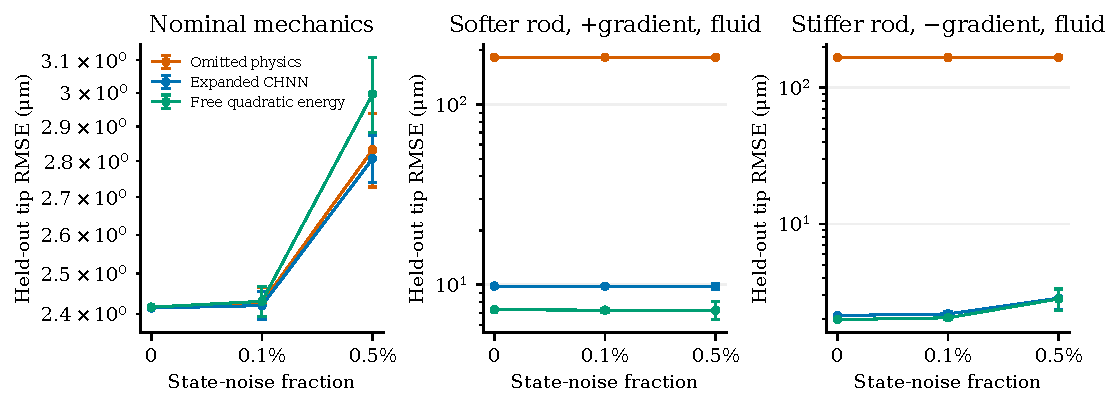
\includegraphics[width=\textwidth]{figures/robustness_noise_and_mismatch.pdf}
\caption{State noise and physics outside the nominal hypothesis class.
Each point averages three independent held-out trajectories. Bars show
the sample standard deviation across three training-noise seeds; the
clean fit is counted once. The higher-error model still re-identifies
its retained parameters.}
\label{fig:robustness-newphysics}
\end{figure*}

\subsection{Causal adaptation to slowly changing unknown parameters}
\label{sec:robustness-causal}
To test time variation separately from recalibration between settings,
we generate a $29$ s full-FE trajectory with a smooth drift. Define
$s=\operatorname{clip}_{[0,1]}((t-4\,\mathrm{s})/(24\,\mathrm{s}))$
and $a=(1-\cos\pi s)/2$. The hidden plant has
$e=0.85+0.20a$, $m=1.20-0.20a$ and
$\alpha/\alpha_{\rm ref}=1.40-0.40a$, while $G=0.5$ T/m and
$c_2=0.02$ kg/m$^2$ remain fixed. Multisine excitation continues
throughout. At cutoffs $8,12,16,20,24,28$ s, each estimator receives
only the preceding $4$ s of positions, velocities and known input.
It then predicts the next $1$ s from the currently observed state.
The coefficients are frozen before future state labels are accessed.

A constant sliding-window fit and a locally affine coefficient fit use
the same weak identity~\eqref{eq:robust-weakfit}; the latter adds features
multiplied by $(t-t_{\rm cut})/(4\,\mathrm{s})$. Linear constraints
preserve the nonnegative readouts over both the fitting interval and
the forecast interval. The known future input is supplied to all
predictors, but future states and true parameter values are withheld.
Across the six forecasts, the mean next-second tip RMSE is $387.483$
$\mu$m for the initial fit frozen at $4$ s, $59.217$ $\mu$m for causal
constant refitting and $9.867$ $\mu$m for causal affine adaptation.
The affine errors range from $2.701$ to $17.295$ $\mu$m. Constant
refitting is better at the final cutoff, where the physical drift
stops; this limitation of extrapolating a local trend is retained.
These are six forecasts on one declared drift trajectory, not independent
patient experiments or a general online-learning theorem.

\begin{figure}[t]
\centering
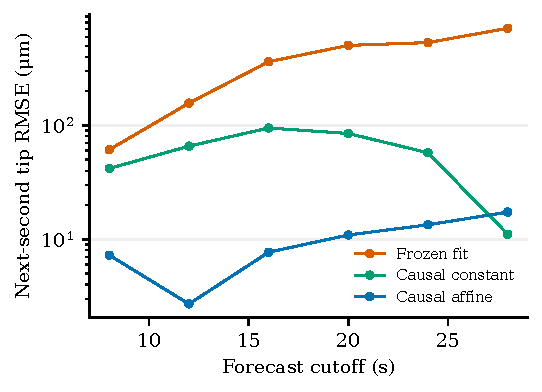
\includegraphics[width=\columnwidth]{figures/causal_parameter_adaptation.pdf}
\caption{One-second forecasts made using only past data under slow
material and magnetic drift. The frozen, constant and affine predictors
share the same current observed state and prescribed future input.}
\label{fig:causal-parameter-adaptation}
\end{figure}

For this nonautonomous plant, the physical energy ledger includes
$E_0[\dot e X^{\mathsf T}A_{\rm el}X/2+\dot m(1-\cos\vartheta)
-\dot g(G_{\rm ref}/B_0)(\ell^{\mathsf T}X)\sin\vartheta]$
in addition to magnetic input power and fluid losses. Its maximum
numerical residual is $6.06\times10^{-14}$ J. The stationary
conservative KAM certificates are not transferred to these driven,
dissipative, time-dependent trajectories.

\subsection{Forced-response stability and clearance boundaries}
\label{sec:stability-boundary}
To distinguish resonance amplification from a dynamical loss of stability,
we additionally scan the same nominal beam under a prescribed transverse
field. This experiment concerns attracting responses of a driven, damped
system; it does not measure destruction of the conservative KAM torus.
The physical parameters, frozen static-field modes and mass-drag coefficient
$\alpha=0.5555852368\,\mathrm{s}^{-1}$ are unchanged. No field-gradient
input, learned-model substitution, governor or contact force is used.
In physical time, the retained modal equations are
\begin{equation}
\begin{aligned}
 \dot X_j&=\omega_jY_j,\\
 \dot Y_j&=-\omega_jX_j-\alpha Y_j\\
 &\quad+\omega_0d_j[\vartheta-\sin\vartheta+u(t)\cos\vartheta],
\end{aligned}
\label{eq:boundary-modal-plant}
\end{equation}
where $\vartheta=d^{\mathsf T}X$, $u=B_y/B_0$, $B_0=30$ mT and
$\omega_0=11.417287283\,\mathrm{rad\,s^{-1}}$.

\paragraph{Fixed protocol and stability diagnostics.}
Independent runs use
$B_y=A[1-\exp(-(t/(0.25\,\mathrm{s}))^2)]\sin(r\omega_0t)$.
The amplitude set is $A\in\{1,2,4,6,10,15,20\}$ mT.
The frequency set contains the $0.02$ grid over $[0.70,1.30]$ and
the $0.005$ grid over $[0.94,1.06]$, giving $49$ distinct ratios.
For each pair, the initial low state is either zero or
$\pm(0.18,0.04,0,0)$, giving $1029$ independent integrations.
Increasing- and decreasing-frequency continuations add $686$ runs.
Each continuation changes frequency at the zero-field phase and inherits
the previous endpoint; the ramp is applied only at its first frequency.
Each run discards $128$ forcing periods and measures the next $64$,
for a total duration of $81.28$--$150.95$ s. Fixed-step DOP853 uses
$256$ steps per forcing period in the two-mode grid.

We integrate the analytic variational equation simultaneously, renormalize
one tangent vector every period, and average its logarithmic growth over
the last $64$ periods. These conditional finite-time Lyapunov exponents
hold the prescribed forcing phase fixed. We also integrate the complete
$4\times4$ fundamental matrix over a further period with $512$ steps,
and calculate the Floquet multipliers of every converged two-mode orbit.
The nontrivial Jacobian block is
\begin{equation}
 D_X\dot Y=-\operatorname{diag}(\omega_j)
 +\omega_0[1-\cos\vartheta-u\sin\vartheta]dd^{\mathsf T}.
\label{eq:boundary-variational-block}
\end{equation}
The identity $\det\mathcal M=\exp(-2\alpha T)$ for its monodromy
matrix supplies an independent numerical check.

All $1715$ runs converge to forcing-periodic responses. The largest
single-period canonical residual is $6.65\times10^{-11}$; the maximum
endpoint differences among the three initial states and between the two
continuation directions are $2.31\times10^{-11}$ and
$4.01\times10^{-11}$, respectively. Conditional exponents in the
independent grid range from $-0.28046$ to $-0.27044\,\mathrm{s}^{-1}$.
Floquet spectral radii range from $0.803809$ to $0.889055$, with the
determinant identity accurate to $1.41\times10^{-14}$.
Fifteen cases at amplitudes $2$, $6$ and $20$ mT and frequency ratios
$0.8$, $0.95$, $1$, $1.05$ and $1.2$ retain periodic recurrence and
negative conditional exponents when both the integration time and
steps per period are doubled, and separately with four and eight modes.
The latter use $1024$ and $4096$ steps per period. Time refinement
changes the sampled two-mode steady peak by at most
$3.81\times10^{-7}$ mm. An independently written adaptive DOP853
implementation also agrees in canonical state to $3.13\times10^{-13}$
on three twelve-period checks.

These are numerical local-stability and basin checks at specified points,
not a proof over a continuous parameter set. Of the $1029$ independent
runs, $550$ keep their sampled whole-beam slope bound below $0.1$ rad
throughout startup and measurement. We use this value as a conservative
reporting screen for the small-slope model, not as a calibrated physical
validity threshold. Large-amplitude rows are retained in the data and
marked in Figure~\ref{fig:stability-boundaries}, but do not establish
physical device performance. No resolved multistability or chaos is
detected in this scan; neither a chaos threshold nor conservative-torus
breakup is inferred from it.

\paragraph{Full-model resonance and clearance contours.}
To resolve the operational boundary without high-mode truncation, we
separately calculate periodic responses using all $64$ frozen FE modes.
For $f=\vartheta-\sin\vartheta+u\cos\vartheta$ with Fourier coefficients
$f_k$ and $\Omega=r\omega_0$, the exact linear modal response is
\begin{equation}
 X_{j,k}=\frac{\omega_0\omega_jd_j f_k}
 {\omega_j^2-(k\Omega)^2+\mathrm i\alpha k\Omega}.
\label{eq:boundary-fourier-response}
\end{equation}
Iterating this response with the nonlinear force gives a numerical
periodic solution; its full nonlinear ODE residual is checked after
reconstructing $\vartheta=d^{\mathsf T}X$. Amplitude root-finding then
locates a $4$ mm peak-displacement crossing at $31$ of $35$ frequency
ratios; the remaining four ratios, $1.225$--$1.30$, have no such crossing
below $20$ mT on the calculated branch. Cubic-Hermite Bernstein bounds
cover every centreline point at each sampled phase. At every reported
crossing these spatial upper bounds equal the actual tip peak to
$8.9\times10^{-16}$ mm, so the contour also locates a tip reaching
$4$ mm in the numerical periodic solution.

\begin{table}[t]
\centering\small
\caption{Numerical $4$ mm crossing amplitudes in mT. Steady crossings
use all $64$ modes. Startup crossings use eight modes, zero initial
state, the stated $0.25$ s ramp, and $192$ forcing periods. They are
protocol-dependent response contours, not certified safe-field limits.}
\label{tab:stability-boundaries}
\begin{tabular}{rrr}
\toprule
$\Omega/\omega_0$ & Steady & Startup\\
\midrule
$0.8$ & $13.6362$ & $8.6513$\\
$0.9$ & $7.5005$ & $5.1882$\\
$1.0$ & $1.9168$ & $1.9169$\\
$1.1$ & $8.7909$ & $5.7662$\\
$1.2$ & $18.5936$ & $10.4455$\\
\bottomrule
\end{tabular}
\end{table}

The steady contour has a numerical minimum near
$r=0.999245$ ($\Omega=11.408664\,\mathrm{rad\,s^{-1}}$), at
$A=1.915911$ mT and a spatial slope bound of $0.06750$ rad.
Thus a $20$ mT actuator limit alone cannot ensure clearance near resonance.
At five representative crossings, increasing the Fourier phase grid
from $1024$ to $4096$ changes the peak by at most $0.00526\,\mu$m.
Comparisons with $2$, $4$, $8$, $16$ and $32$ modes are retained:
at these same inputs the two-mode peak differs from the full FE peak
by up to $67.73\,\mu$m, whereas the eight-mode discrepancy is below
$4.18\,\mu$m. Independent full-FE Radau integration from the computed
periodic states at $r=0.8,1,1.2$ agrees in tip position to
$1.11\times10^{-12}$ m over one period.

Startup overshoot imposes a different contour. The eight-mode startup
roots in Table~\ref{tab:stability-boundaries} use $512$ observation
phases per cycle; doubling time, integration resolution and observation
resolution at $r=0.8,1,1.2$ changes the peak by at most
$0.0678\,\mu$m. Full-FE integration from rest over the first $32$
periods, combined with the separately computed periodic response,
changes the checked peak by at most $2.44\,\mu$m. At $r=0.8$, the
approximately $8.6513$ mT request has a $2.5411$ mm full-FE steady
amplitude but reaches $4.0020$ mm during startup. This is a numerical
overshoot example with no wall-contact force. The continuous-time
input-work governor of Section~\ref{sec:unifiedsafety} remains the
proved clearance mechanism; the response contours explain why both
frequency and startup must enter a practical operating choice.

\begin{figure*}[t]
\centering
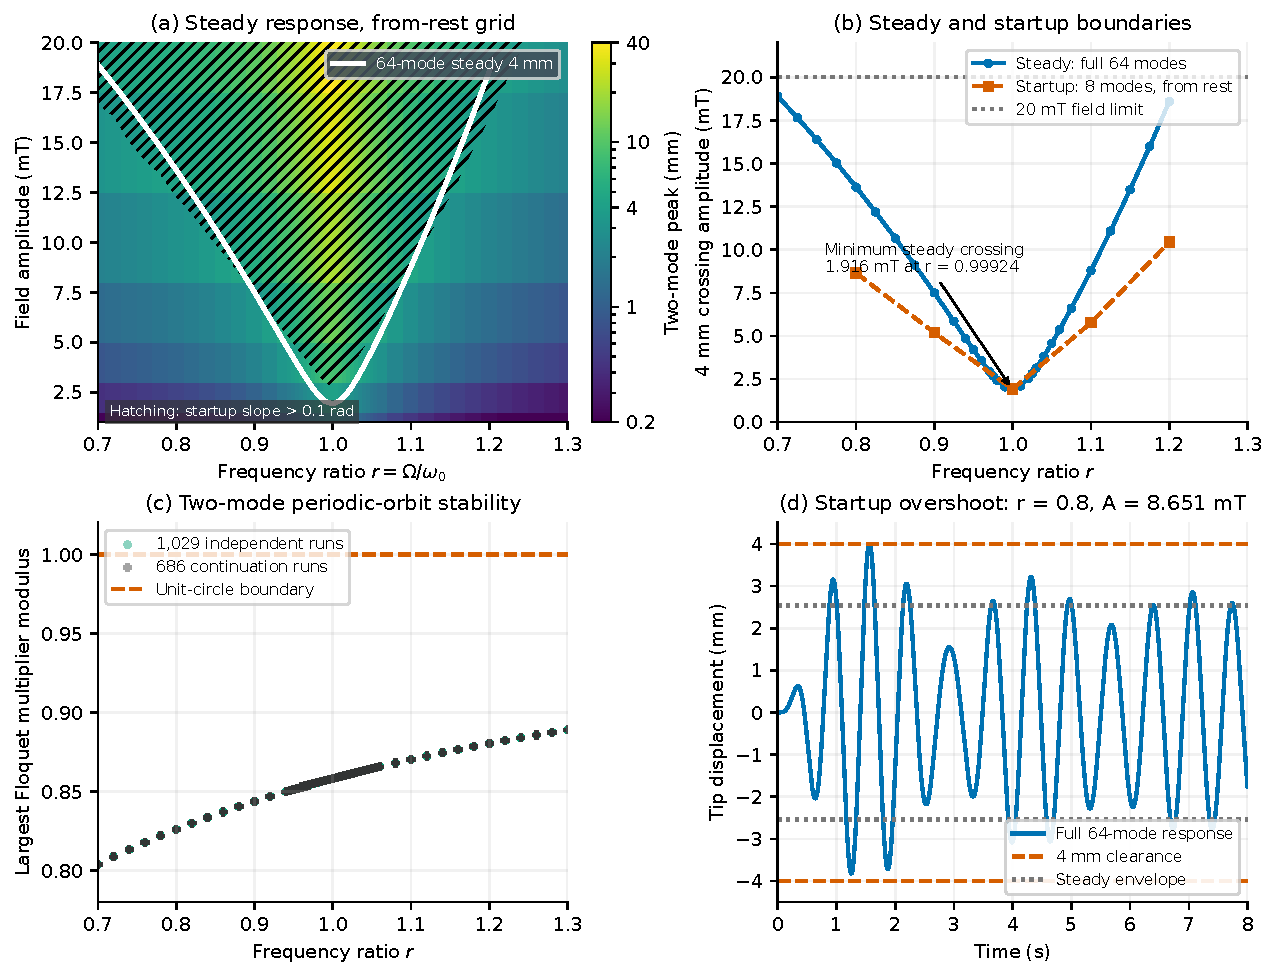
\includegraphics[width=\textwidth]{reproducibility/reviewer_revision_20261008/stability_scan/fig_stability_boundaries.pdf}
\caption{Driven-response and clearance study of the same magnetic beam.
(a) Two-mode steady peak on the from-rest grid; hatching marks sampled
startup slopes above the $0.1$ rad reporting screen. The white line is
the independently computed full-FE steady $4$ mm contour.
(b) Full-FE steady and eight-mode startup contours under the fixed ramp.
(c) Floquet multipliers of the two-mode periodic responses from all
independent and continuation runs. (d) Full-FE startup overshoot near
the eight-mode numerical crossing. Stability of an attracting forced
periodic response is distinct from conservative KAM-torus persistence.}
\label{fig:stability-boundaries}
\end{figure*}


\section{Preserving KAM dynamics through magnetic actuation}
\label{sec:kam-actuation}
\subsection{Magnetic feedback that preserves the learned KAM dynamics}
\label{sec:full-fe-kam-control}
A spatial magnetic-field gradient supplies a tip-force input that, together
with the transverse field, preserves the certified conservative dynamics
despite physical damping. Both inputs act through the magnetic dipole
on the same finite-element beam.

Let $a_j$ be the physical mass-normalized modal positions of the complete
$64$-mode FE model, with velocities $v_j$, frequencies $\omega_j$,
tip-displacement participation $b_j$, and tip-rotation participation $t_j$.
The numerical theorem uses the exported modal coefficients and Hermite
shape map as the exact definition of the computational model. The
diagonalization residual relative to the assembled nodal matrices is
quantified below.
Write $\vartheta=\sum_jt_ja_j$ and $E_0=\mu B_0$. With transverse tip
force $F$ and transverse field $B_y$, the modal equations are
\begin{equation}
 \begin{aligned}
 \ddot a_j+\alpha\dot a_j+\omega_j^2a_j&=b_jF+t_jU,\\
 U&=E_0(\vartheta-\sin\vartheta)+\mu B_y\cos\vartheta.
 \end{aligned}
 \label{eq:full-fe-two-port}
\end{equation}
The frequencies already include the linear stiffness from $B_0$.
For the first two modes define
\begin{equation}
 A_{\rm mag}=\begin{pmatrix}b_1&t_1\\b_2&t_2\end{pmatrix}.
 \label{eq:magnetic-authority-matrix}
\end{equation}
An interval enclosure of its determinant excludes zero.

Let $h(X,Y)$ be the fitted Hamiltonian used by the KAM
certificate, including momentum-dependent quartics. Set
$a_i=S_iX_i$ and recover $Y$ from
\begin{equation}
 h_Y(X,Y)=\operatorname{diag}(S_i)^{-1}v_{1:2}/\omega_0.
 \label{eq:full-fe-legendre}
\end{equation}
This implicit velocity-to-momentum map cannot be replaced by $Y_i=v_i/(S_i
\omega_0\nu_i)$ when the learned momentum quartics are retained. The
verified lower bound on $h_{YY}$ below makes the map locally invertible and
injective in $Y$ on the stated real box. Define
\begin{align}
 a^{\rm des}_{i,tt}
 &=S_i\omega_0^2\bigl(h_{YX}h_Y-h_{YY}h_X\bigr)_i,\\
 \begin{pmatrix}F\\U\end{pmatrix}
 &=A_{\rm mag}^{-1}
   \left(a^{\rm des}_{1:2,tt}+\alpha v_{1:2}
          +\operatorname{diag}(\omega_1^2,\omega_2^2)a_{1:2}\right).
 \label{eq:full-fe-hamiltonian-feedback}
\end{align}
Consequently $\dot X=\omega_0h_Y$ and $\dot Y=-\omega_0h_X$ exactly
where the implicit inverse is defined. The proof follows by differentiating
\eqref{eq:full-fe-legendre}: the specified acceleration cancels the $h_{YX}$
term and invertibility of $h_{YY}$ gives the second canonical equation.

The physical commands realizing \eqref{eq:full-fe-hamiltonian-feedback} are
\begin{equation}
 \begin{aligned}
 B_y&=\frac{U-E_0(\vartheta-\sin\vartheta)}{\mu\cos\vartheta},\\
 G&=\frac{F}{\mu}
 \begin{pmatrix}-\sin\vartheta&\cos\vartheta\\
                 \cos\vartheta&\sin\vartheta\end{pmatrix}.
 \end{aligned}
 \label{eq:physical-gradient-command}
\end{equation}
Use $B(r)=B_{\rm tip}+G(r-r_{\rm tip})$ locally, with
$B_{\rm tip}=(B_0,B_y)$. The matrix $G$ is symmetric and traceless,
so this local planar field satisfies the source-free curl and divergence
constraints. For dipole $m=\mu(\cos\vartheta,\sin\vartheta)$ it gives
$Gm=(0,F)$, while the tip torque is
$\mu(B_y\cos\vartheta-B_0\sin\vartheta)$.
Moreover $\|G\|_2=|F|/\mu$. The applied mechanical power is
$F\dot w(L)+\mu B_y\cos\vartheta\,\dot\vartheta$, in addition to
the static magnetic energy already included in the Hamiltonian.
The construction assumes these local field and gradient commands are
available and the required modal and tip states are observed.

\subsection{Lifting a certified torus to the complete controlled FE model}
\label{sec:full-fe-kam-lift}
\begin{theorem}[Invariant-torus lift under physical magnetic feedback]
\label{thm:full-fe-kam-lift}
Suppose a real analytic embedded two-torus $K_\infty$ of $h$ has frequency
$\Omega\in\mathbb R^2$ in radians per physical second. Suppose $h_{YY}$
is positive definite on a neighbourhood of this torus with convex
$Y$-fibres for each $X$, $A_{\rm mag}$ is invertible,
$\alpha>0$, and the complete lifted solution has
$|\vartheta|<\pi/2$. Then the full FE closed loop
\eqref{eq:full-fe-two-port}--\eqref{eq:physical-gradient-command} has an
embedded invariant two-torus projecting to $K_\infty$. For a fixed low-mode
orbit on this torus, each high-mode solution converges exponentially to a
unique quasiperiodic response, provided the feedback remains in its
stated field and state domain.
\end{theorem}

\begin{proof}
The first two canonical modes follow $h$ exactly. Hence $F$ and $U$ in
\eqref{eq:full-fe-hamiltonian-feedback} depend only on their torus phase,
even though the physical field command also uses the complete tip angle.
For every $j\geq3$, the remaining dynamics are the stable linear equation
\eqref{eq:full-fe-two-port}, forced by analytic quasiperiodic functions.
If $F_k,U_k$ denote their Fourier coefficients in the convention
$e^{ik\cdot\phi}$, the unique response graph is
\begin{equation}
 a^*_{j,k}=
 \frac{b_jF_k+t_jU_k}
      {\omega_j^2-(k\cdot\Omega)^2+i\alpha(k\cdot\Omega)}.
 \label{eq:full-fe-lift-fourier}
\end{equation}
For real $k\cdot\Omega$, this denominator never vanishes: at zero
frequency its real part is $\omega_j^2>0$, and at nonzero frequency its
imaginary part is nonzero. Its inverse is uniformly bounded over real
frequencies. Exponential Fourier decay is therefore preserved on a
possibly smaller analytic strip. The velocity graph is obtained by
multiplication by $ik\cdot\Omega$ and is analytic on a smaller strip.
Positive definiteness on each convex $Y$-fibre makes
$Y\mapsto h_Y(X,Y)$ strictly monotone and injective. Thus the physical
low-mode positions and velocities preserve the injective canonical
embedding. Differences in the high modes obey the
homogeneous damped equations and decay exponentially.
\end{proof}

The lifted closed loop combines Hamiltonian low-mode motion with
contracting high-mode fibres. The contraction leaves each initial low-mode
torus invariant; it does not select a unique torus or make the full
controlled system Hamiltonian. Each lifted two-torus has zero volume in
the full $128$-dimensional phase space. The KAM-family measure therefore
refers to the conservative low-mode coordinates.

\paragraph{All-phase response and startup bounds.}
We bound both the response graph and the startup
with all high modal positions and velocities initially zero. Write
$h=h_2+R$, and let the certified torus satisfy
$\|K_\infty-K_0\|_\infty\leq\epsilon_K$, where
$K_0=0.1(\cos\phi_1,\cos\phi_2,-\sin\phi_1,-\sin\phi_2)$.
The first two components of the force demand can be written as
\begin{align}
 r_i={}&S_i\bigl\{\omega_0^2[
 (R_{YX}h_Y)_i-\nu_iR_{X_i}-(R_{YY}h_X)_i]\nonumber\\
 &\quad+\alpha\omega_0h_{Y_i}
 +(\omega_i^2-\omega_0^2\nu_i^2)X_i\bigr\},
 \label{eq:full-fe-small-force}
\end{align}
This identity cancels the large linear restoring terms before bounding.
The linear part on $K_0$ consists of just the two known physical
frequencies. Each is bounded using its actual damped denominator in
\eqref{eq:full-fe-lift-fourier}. The remaining terms are bounded on
$|X_i|,|Y_i|\leq0.1+\epsilon_K$ using every fitted quartic coefficient and
the complete trigonometric remainder bounds
$|\sin z-z|\leq|z|^3/6$ and $|1-\cos z|\leq z^2/2$ for real $z$.

For $\beta=\alpha/2$ and
$\omega_{d,j}=\sqrt{\omega_j^2-\beta^2}>0$, the impulse response
$g_j(t)=e^{-\beta t}\sin(\omega_{d,j}t)/\omega_{d,j}$ obeys
\begin{equation}
 \|g_j\|_{L^1(0,\infty)}\leq\frac{2}{\alpha\omega_{d,j}},
 \qquad
 \|g_j'\|_{L^1(0,\infty)}\leq\frac2\alpha+\frac1{\omega_{d,j}}.
 \label{eq:full-fe-green-bounds}
\end{equation}
These estimates include the entire nonlinear forcing remainder and its
Fourier tail. Let $P_j,V_j$ be the resulting all-phase
bounds on the graph's position and velocity. Starting high mode $j$ at
zero adds at most
\begin{equation}
 T_j=P_j+\frac{V_j+\beta P_j}{\omega_{d,j}}
 \label{eq:full-fe-transient}
\end{equation}
to its position envelope. This follows from the exact homogeneous
solution initialized by $(-a_j^*(0),-\dot a_j^*(0))$.
The bounds sum all $62$ high modes and use the cubic Bernstein
control rows of every Hermite element to convert these modal envelopes
into bounds on every centreline point and every phase.

For the two-mode COMSOL integral fit in
Section~\ref{sec:validated-integral-learning}, which satisfies the
nonzero-loss and finite-amplitude KAM conditions, 256-bit Arb
arithmetic encloses $h_{YY}\succeq0.9999999983I$ on the real $0.3$ box.
The complete response graph has centreline amplitude below $1.922696$ mm.
Including the zero-high-mode startup yields an all-time bound below $1.970263$ mm,
strictly inside the $4$ mm net corridor. The latter envelope gives
$|\vartheta|<0.155261$ and $\cos\vartheta>0.987971$, which closes the
feedback-domain bootstrap. The required transverse field is below
$0.921665$ mT and the gradient spectral norm below
$0.02572538\,\mathrm{T\,m^{-1}}$ at every phase and throughout that
startup. These bounds validate feasibility under a $20$ mT transverse
field limit and a $1\,\mathrm{T\,m^{-1}}$ gradient limit; they are
derived bounds, not the extrema of a simulated time history.
Applying the same computation to the fit trained on complete COMSOL FE
trajectories in Section~\ref{sec:comsol-identification} gives graph and
zero-high-state startup bounds of $1.937308$ mm and $2.014078$ mm,
respectively.

The theorem applies to initial low states on the exact certified torus.
The numerical Fourier initial state approximates it within the
certified KAM correction, and finite-time integration tests the feedback
implementation. The theorem uses the exported modal FE coefficients and
fitted weights; independent COMSOL comparisons assess the corresponding
nodal mechanical implementation.
To make the modal definition explicit, if $\Phi$ is the stored full
shape basis, $M,K_b$ are the independently assembled nodal matrices and
$D_\omega=\operatorname{diag}(\omega_j)$, outward Arb products give
\begin{align}
 \|\Phi^{\mathsf T}M\Phi-I\|_\infty&<1.304685\times10^{-14},\\
 \|D_\omega^{-1}\Phi^{\mathsf T}K_b\Phi D_\omega^{-1}-I\|_\infty
 &<3.000518\times10^{-9}.
\end{align}
These are relative kinetic- and stiffness-energy form bounds. They
quantify the relationship between the frozen modal model and the
original assembled FE representation; they are not used to assert
an exact conjugacy or an unproved persistence result for perturbed
matrices. The two-mode shape map used for identification differs from the
reassembled map by at most $1.258\times10^{-14}$ m, and the reference
frequency $\omega_0$ is unchanged.

\subsection{Full-model implementation and frequency preservation}
\label{sec:kam-control-experiment}
The feedback is integrated on all $64$ modes for $12$ s, using the
two-mode COMSOL integral fit certified in
Section~\ref{sec:validated-integral-learning}. The initial low state is
the phase-zero Fourier candidate and all higher modal positions and
velocities are zero. A separate high-accuracy integration of the
four-dimensional learned Hamiltonian supplies an implementation
reference. The plant is actuated through the physical tip force and moment.
The maximum canonical state difference is $1.54\times10^{-10}$,
the relative learned-energy change is below $2.64\times10^{-9}$,
and the full physical work-balance residual is below
$6.06\times10^{-17}$ J. The sampled field and gradient peaks are
$0.890325$ mT and $0.0256844$ T/m. Figure~\ref{fig:kam-magnetic-control}
compares this trajectory with the same initial state under passive
damping, for which the learned energy decreases by $99.8726\%$.
The numerical trajectory is an implementation check; the all-time
envelopes come from the preceding interval proof.
An independent implementation integrates the low Hamiltonian separately
and propagates each of the $62$ high damped oscillators by its exact
exponential response to piecewise-linear force demands. Force-grid
steps of $1$, $0.5$ and $0.25$ ms give maximum tip differences from the
full-state integration of $1.073$, $0.277$ and $0.106$ nm, respectively.
Every high-mode homogeneous transient is retained. This check separates
time-step error from modal truncation and supports the full-state
implementation. The resulting differences measure numerical convergence;
the rigorous bounds are supplied by the interval proof.

\paragraph{Independent online COMSOL feedback.}
The complete nodal beam is also solved with the CHNN feedback inside
COMSOL. The first two modal coordinates and velocities are projected
from its current beam state; two global algebraic equations enforce
the learned Legendre inverse. The physical tip force and magnetic
moment are recomputed online. This experiment is distinct from the
prescribed-field S-path replay.
Generalized-alpha integration uses $\rho_\infty=0$, a nonlinear relative
tolerance of $10^{-8}$ and fixed steps. Table~\ref{tab:comsol-kam-refinement}
reports four $4$ s refinements and compares them at common sampled
times with the independent full-state Python run.
At the finest step, the maximum relative change in the learned energy
is $0.0002958$. These numerical
errors are reported separately from the analytic KAM and all-time
amplitude certificates. Adaptive stepping stalled at very small steps
in two preliminary runs; fixed stepping completed each refinement.

\begin{table}[t]
\centering\small
\caption{Online COMSOL feedback versus independent Python
integration. Errors are in $\mu$m; no step-size tolerance is interpreted
as a rigorous error bound.}
\label{tab:comsol-kam-refinement}
\begin{tabular}{rrr}
\toprule
Step (ms) & Tip RMSE & Maximum tip difference\\
\midrule
1 & 147.852 & 355.845\\
0.5 & 41.356 & 99.176\\
0.25 & 12.006 & 28.161\\
0.125 & 3.848 & 8.658\\
\bottomrule
\end{tabular}
\end{table}

The two certified physical angular frequencies are approximately
$11.41719351$ and $70.24034116$ rad/s. Their exact specification and
all-integer Diophantine bound follow from the KAM certificate under
the stated time normalization. Magnetic feedback
therefore preserves a certified nonresonant frequency pair while
compensating damping. The complete nonlinear command contains the
harmonics determined by the torus; it is not approximated by two
sinusoidal inputs when invoking the lifting theorem. The rigorous
state and command envelopes provide a simultaneous amplitude check.
The operating-domain fraction is examined separately in
Section~\ref{sec:measure-numerical}.

\begin{figure*}[t]
\centering
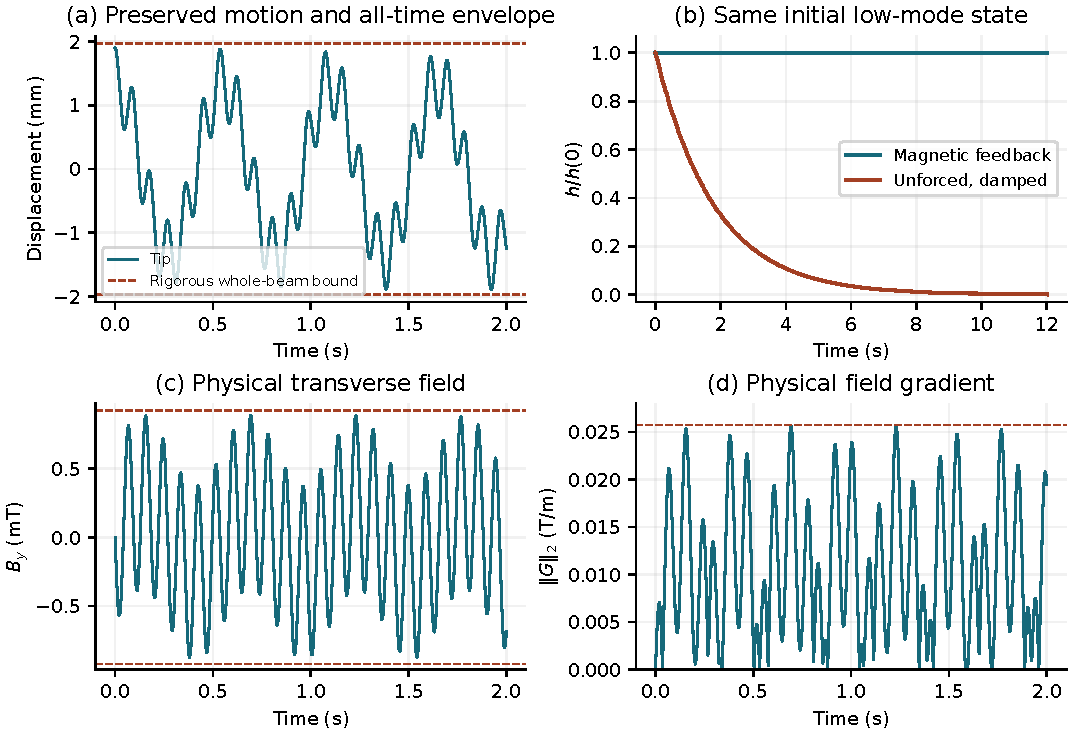
\includegraphics[width=\textwidth]{figures/fig_kam_magnetic_control.pdf}
\caption{Magnetic preservation of the COMSOL-integral learned
Hamiltonian on the complete exported modal FE plant. The higher modes
start at zero and undergo a decaying transient toward their unique
quasiperiodic response graph. Dashed bounds in (a), (c) and (d) are
validated all-phase bounds, including that startup. The field and
gradient in (c,d) jointly realize physical tip force and torque.
Panels (a,c,d) show the first $2$ s; panel (b) shows the complete $12$ s run.}
\label{fig:kam-magnetic-control}
\end{figure*}


\section{Clearance guarantees and magnetic safety control}
\label{sec:safety}
\subsection{A whole-beam clearance certificate for the same magnetic model}
\label{sec:unifiedsafety}
The conservative normal form and the safety calculation use the same
clamped-free beam, static field, magnetic dipole, and energy.  Safety is a
statement about the driven physical equations, with their nonnegative drag;
it does not require a driven trajectory to lie on a conservative KAM torus.
For the planar, small-slope model, write $w(s,t)$ for transverse
displacement, $m=\rho A$ for line density, $c_d\geq0$ for distributed viscous
drag, and $\vartheta=w_s(L,t)$ for the tip slope used in the dipole potential.
The equations and natural end conditions are
\begin{align}
 m w_{tt}+c_d w_t+EIw_{ssss}&=0,\qquad 0<s<L,\\
 w(0,t)=w_s(0,t)&=0,\qquad w_{sss}(L,t)=0,\\
 EI w_{ss}(L,t)&=\mu\{B_y(t)\cos\vartheta-B_0\sin\vartheta\}.
 \label{eq:unifiedbeamportBC}
\end{align}
The end moment is the derivative of the same cosine potential used to
generate the training trajectories.  In particular, the varying transverse
field is an input port, not an additional autonomous Hamiltonian perturbation.
For a sufficiently regular solution satisfying the mechanical power identity,
the stored energy relative to the aligned static-field equilibrium is
\begin{align}
 E(t)&=\frac12\int_0^L\{m w_t^2+EIw_{ss}^2\}\dd s
        +\mu B_0(1-\cos\vartheta),\\
 \dot E&=-c_d\int_0^L w_t^2\dd s
             +\mu B_y\cos\vartheta\,\dot\vartheta.
 \label{eq:unifiedSIpower}
\end{align}
All inequalities below also hold for the conforming cubic-Hermite finite
element (FE) system and any of its Galerkin subspaces, because their energies
are the restrictions of this expression and retain the same input power.
In the balanced coordinates of the learning experiment, $E=\mu B_0 h_*$
for the physical target energy,
$\vartheta=d^{\mathsf T}X$, and the port force in the $Y$ equation is
$d(B_y/B_0)\cos(d^{\mathsf T}X)$.

\begin{proposition}[Clearance and field-variation budget]
\label{prop:unifiedvariation}
Assume $B_0>0$, $c_d\geq0$, and an absolutely continuous applied field
$B_y$ on $[0,T]$.  Define
\begin{align}
 S_T&=\sup_{0\leq t\leq T}|B_y(t)|+|B_y(0)|\notag\\
    &\quad+\int_0^T|\dot B_y(t)|\dd t,\\
 C_T&=\mu\sqrt{\frac{2L}{EI}}S_T,
 \\
 R_T&=\frac{C_T+\sqrt{C_T^2+4E(0)}}{2}.
 \label{eq:unifiedvariationbudget}
\end{align}
Then, throughout $[0,T]$,
\begin{equation}
 \begin{aligned}
 E(t)&\leq R_T^2,\\
 |w(s,t)|&\leq\sqrt{\frac{2s^3}{3EI}}R_T,\\
 |w_s(s,t)|&\leq\sqrt{\frac{2s}{EI}}R_T.
 \end{aligned}
 \label{eq:unifiedcontinuumshape}
\end{equation}
For a straight corridor with wall half-width $a$ and rod radius $r$, let
$c=a-r>0$.  A sufficient condition for positive clearance of the whole
rod is $R_T<\sqrt{E_c}$, where
\begin{equation}
 E_c=\frac{3EIc^2}{2L^3}.
 \label{eq:unifiedclearanceenergy}
\end{equation}
For $E(0)<E_c$, the following directly checkable operating condition is
equivalent to this sufficient energy condition:
\begin{equation}
 S_T<\frac{E_c-E(0)}{\mu\sqrt{2LE_c/EI}}.
 \label{eq:unifiedoperationbudget}
\end{equation}
These conclusions hold for every nonnegative drag coefficient, including zero.
\end{proposition}

\begin{proof}
Since $B_0>0$, the static magnetic energy is nonnegative and
$\|w_{ss}\|_{L^2}^2\leq2E/EI$.
The clamped conditions imply
$w(s)=\int_0^s(s-\xi)w_{ss}(\xi)\dd\xi$ and
$w_s(s)=\int_0^s w_{ss}(\xi)\dd\xi$.
Cauchy--Schwarz gives the two spatial inequalities in
\eqref{eq:unifiedcontinuumshape} with $\sqrt E$ in place of $R_T$.
Write $D_c(t)=\int_0^t c_d\|w_t\|_{L^2}^2\dd\tau$.
Integrating \eqref{eq:unifiedSIpower} by parts in the input term gives
\begin{align*}
 &E(t)+D_c(t)-E(0)\\
 &\quad=\mu B_y(t)\sin\vartheta(t)\\
 &\qquad-\mu B_y(0)\sin\vartheta(0)\\
 &\qquad-\mu\int_0^t\dot B_y(\tau)\sin\vartheta(\tau)\dd\tau.
\end{align*}
Set $M_T=\sup_{[0,T]}\sqrt{E(t)}$.
Using $|\sin\vartheta|\leq|\vartheta|
\leq\sqrt{2L/EI}\,M_T$ and discarding the nonnegative dissipation yields
$M_T^2\leq E(0)+C_TM_T$.
The positive root is $R_T$.
The entire radius-$r$ tube about the centerline remains between the walls
when $\sup_s|w(s,t)|<a-r$.
Solving $R_T<\sqrt{E_c}$ gives
\eqref{eq:unifiedoperationbudget}.
\end{proof}

For a nonuniform planar corridor, let $c(s)>0$ be the Euclidean distance
from the undeformed point $(s,0)$ to the wall, less the rod radius.
The distance-to-wall function is one-Lipschitz, so $|w(s)|<c(s)$
keeps the radius-$r$ tube clear. The same argument replaces $E_c$ by
$\inf_{0<s\leq L}3EIc(s)^2/(2s^3)$.
For an inclined or curved wall, a local vertical half-width is not
a substitute for this Euclidean clearance.
This sufficient condition applies to the specified corridor geometry;
vessel-specific use requires its own wall data. The continuum inequality
applies directly to solutions with the stated initial-energy and
applied-field bounds, and holds separately for conforming FE solutions.
It therefore requires neither a two-mode reconstruction error estimate
nor an identification of an FE trajectory with a continuum solution.

For the shared SI parameters, choose $a=4.6$ mm and $r=0.6$ mm, so that
$c=4$ mm.  The resulting $E_c$ is $23.8565$ nJ.
For a monotone field ramp from zero to $A$ followed by a hold,
$S_\infty=2A$.  With zero initial energy, a sufficient condition is
\begin{equation}
 A<\frac{\sqrt3\,EIc}{4\mu L^2}=6.8868\ \mathrm{mT}.
 \label{eq:unifiedramplimit}
\end{equation}
For $B_y=A\rho(t)\sin(\Omega t)$ with
$\rho(t)=1-\exp[-(t/0.25\,\mathrm{s})^2]$,
$S_T\leq A(2+\Omega T)$, because $\rho$ increases from zero and is at most
one.  Thus amplitude, frequency and operating duration enter an explicit
joint condition by substituting this bound in
\eqref{eq:unifiedoperationbudget}.
For $T=8$ s, $\Omega=9.444949$ rad/s and $E(0)=0$, its sufficient amplitude
limit is approximately $0.1776$ mT.  This conservative open-loop test does
not certify the default $6$ mT sinusoid, even when a simulated trajectory
has positive clearance.

\subsection{A magnetic-input governor with a full-model energy guarantee}
\label{sec:unifiedgovernor}
The field-variation test can be strengthened for feedback operation by
measuring the actual mechanical input port.  Let $\overline E_0\geq E(0)$
be a valid initial-energy bound and integrate
\begin{equation}
 W(t)=\overline E_0+\int_0^t
      \mu B_y\cos\vartheta\,\dot\vartheta\dd\tau.
 \label{eq:unifiedworkobserver}
\end{equation}
Equation~\eqref{eq:unifiedSIpower} gives $E(t)\leq W(t)$ without measuring
or estimating the dissipated energy.  Given $E(0)\leq\overline E_0<E_{\max}<E_c$,
a bounded requested field $|B_{\mathrm{req}}|\leq B_{\max}$, and $\kappa>0$,
choose the applied field as the closest value to $B_{\mathrm{req}}$ satisfying
\begin{equation}
 \begin{aligned}
 |B_y|&\leq B_{\max},\\
 a_p B_y&\leq\kappa(E_{\max}-W),\\
 a_p&=\mu\cos\vartheta\,\dot\vartheta.
 \end{aligned}
 \label{eq:unifiedgovernor}
\end{equation}
This is a scalar projection onto an interval.  Whenever the requested input
violates the work constraint and $a_p\ne0$, the applied field is
$B_y=\kappa(E_{\max}-W)/a_p$; otherwise it is unchanged.
On $W\leq E_{\max}$, zero field is feasible, and this projection never
increases the requested field amplitude.

\begin{proposition}[Port-work safety invariant]
\label{prop:unifiedgovernor}
Suppose the actual applied field and actual tip slope and slope rate are
available to \eqref{eq:unifiedworkobserver}--\eqref{eq:unifiedgovernor},
and the field command is applied without unbudgeted error or delay.
Every closed-loop solution satisfying the mechanical power identity obeys
\begin{equation}
 \begin{aligned}
 E(t)&\leq W(t)\leq E_{\max},\\
 \sup_s|w(s,t)|&\leq\sqrt{\frac{2L^3E_{\max}}{3EI}}<c.
 \end{aligned}
 \label{eq:unifiedgovernorbound}
\end{equation}
Consequently the entire rod retains positive wall clearance for all times
on which the stated beam model and port measurements apply, for any $c_d\geq0$.
\end{proposition}

\begin{proof}
The power identity gives $W-E=\overline E_0-E(0)
+\int_0^t c_d\|w_t\|_{L^2}^2\dd\tau\geq0$.
The input constraint yields
$\dot W\leq\kappa(E_{\max}-W)$, hence
$E_{\max}-W(t)\geq
(E_{\max}-\overline E_0)\exp(-\kappa t)\geq0$.
The spatial estimate proved above completes the result.
\end{proof}

The guarantee uses the full physical input power, including the work
associated with unobserved high modes. A learned model supplies the
requested field. Accurate actual-port measurements and ideal command
application are assumed; sensor, actuation and delay errors require
additional work-error budgets. The projection constrains field amplitude
and accumulated work, with no imposed slew-rate bound. Because dissipated
energy is not credited back, the observer can restrict the request even
when stored energy has decreased. Tracking performance is therefore
evaluated separately under this conservative safety constraint.

A bounded port-measurement error can be included without assuming an exact
learned state.  If $|a_p-\widehat a_p|\leq\delta_a(t)$, replace the observer
derivative and its input constraint by
\begin{equation}
 \begin{aligned}
 \dot W&=\widehat a_p B_y+\delta_a|B_y|\\
       &\leq\kappa(E_{\max}-W).
 \end{aligned}
 \label{eq:unifiedrobustport}
\end{equation}
Actual input power is at most this observer derivative, so the same proof
applies.  Zero field remains feasible and the scalar feasible set is convex.
Here $B_y$ must be the actual applied field; an uncertain command-to-field
map requires a further bound on actual input power.  The numerical tests
below use $\delta_a=0$ and do not experimentally validate a sensor-error bound.

\subsection{Full-FE safety, violation and truncation checks}
\label{sec:unifiedsafetytests}
All tests use the shared $32$-element consistent-mass FE beam, retain all
$64$ unconstrained displacement/slope degrees of freedom, and integrate
the exact cosine tip potential.  The coordinates are the complete
$64$-mode static-field basis; this is a change of coordinates, not a
modal truncation.  The default drag is $C=\alpha M$ with
$\alpha=0.55558524$ s$^{-1}$.  Unless stated otherwise, trajectories start
from rest at the straight equilibrium.  The sinusoidal tests use the
frequency $\Omega=9.444949$ rad/s and the $0.25$ s ramp above; the monotone
tests omit the sine factor.  The integration interval is $8$ s.
The continuous-time claims come from Propositions~\ref{prop:unifiedvariation}
and \ref{prop:unifiedgovernor}; cubic-Hermite spatial extrema are evaluated
exactly at each saved time for the numerical diagnostics.

Table~\ref{tab:unifiedsafety} separates numerical maxima from continuous-time
certificates.  The $6$ mT monotone ramp satisfies an all-time displacement
bound of $3.48494$ mm, including zero drag.  The default $6$ mT sinusoid
has a numerical peak of $3.09031$ mm, but fails the conservative field-variation
test; that peak alone is not a safety proof.  Increasing its amplitude to
$10$ mT produces a $5.14478$ mm free-motion peak and crosses the $4$ mm
boundary.  The continuation after crossing is a diagnostic of a violated
constraint, not a simulation of wall contact.

With $E_{\max}=0.95E_c=22.66365$ nJ and $\kappa=5$ s$^{-1}$,
the work governor applied to the same $10$ mT request has a rigorous
whole-centerline bound of $3.89872$ mm and thus a minimum guaranteed
clearance of $0.10128$ mm.  Its numerical peak is $3.14362$ mm with the
default drag and $3.55853$ mm with zero drag.  The same energy cap also
implies $\sup_s|w_s|\leq0.08441$, consistent with the declared small-slope
regime for the certified trajectories.
Tightening both relative and absolute integration tolerances tenfold
for the full-FE governed case changes the tip trajectory by at most
$8.19\times10^{-11}$ m; the refined power-balance residual is
$3.86\times10^{-18}$ J ($1.74\times10^{-10}$ relative to the work scale).
The governor changes the requested field at $55.37\%$ of saved times
in this oscillatory case.

\begin{table*}[t]
\centering
\caption{Safety tests on the same full $32$-element, $64$-DOF FE beam.
Numerical maxima are cubic-Hermite spatial extrema at $2001$ saved times
over $8$ s.  Bounds are continuous-time sufficient bounds from the stated
propositions.  ``No'' means the sufficient test does not certify the case.
All fields use a $0.25$ s ramp; sine frequency is $9.444949$ rad/s.
Except the stated $E_c/4$ case, initial energy is zero.}
\label{tab:unifiedsafety}
\begin{tabular}{lrrc}
\toprule
Applied protocol & Peak (mm) & Bound (mm) & Certified\\
\midrule
$6$ mT ramp/hold & $0.92405$ & $3.48494$ & Yes\\
$3$ mT ramp, $E(0)=E_c/4$ & $2.06222$ & $3.05276$ & Yes\\
$0.15$ mT sine & $0.07731$ & $3.37863$ & Yes\\
$6$ mT sine & $3.09031$ & $135.145$ & No\\
$10$ mT sine & $5.14478$ & $225.242$ & No\\
Governed $10$ mT sine & $3.14362$ & $3.89872$ & Yes\\
Governed $10$ mT, zero drag & $3.55853$ & $3.89872$ & Yes\\
$6$ mT ramp, zero drag & $0.95405$ & $3.48494$ & Yes\\
\bottomrule
\end{tabular}
\end{table*}

\begin{figure*}[t]
\centering
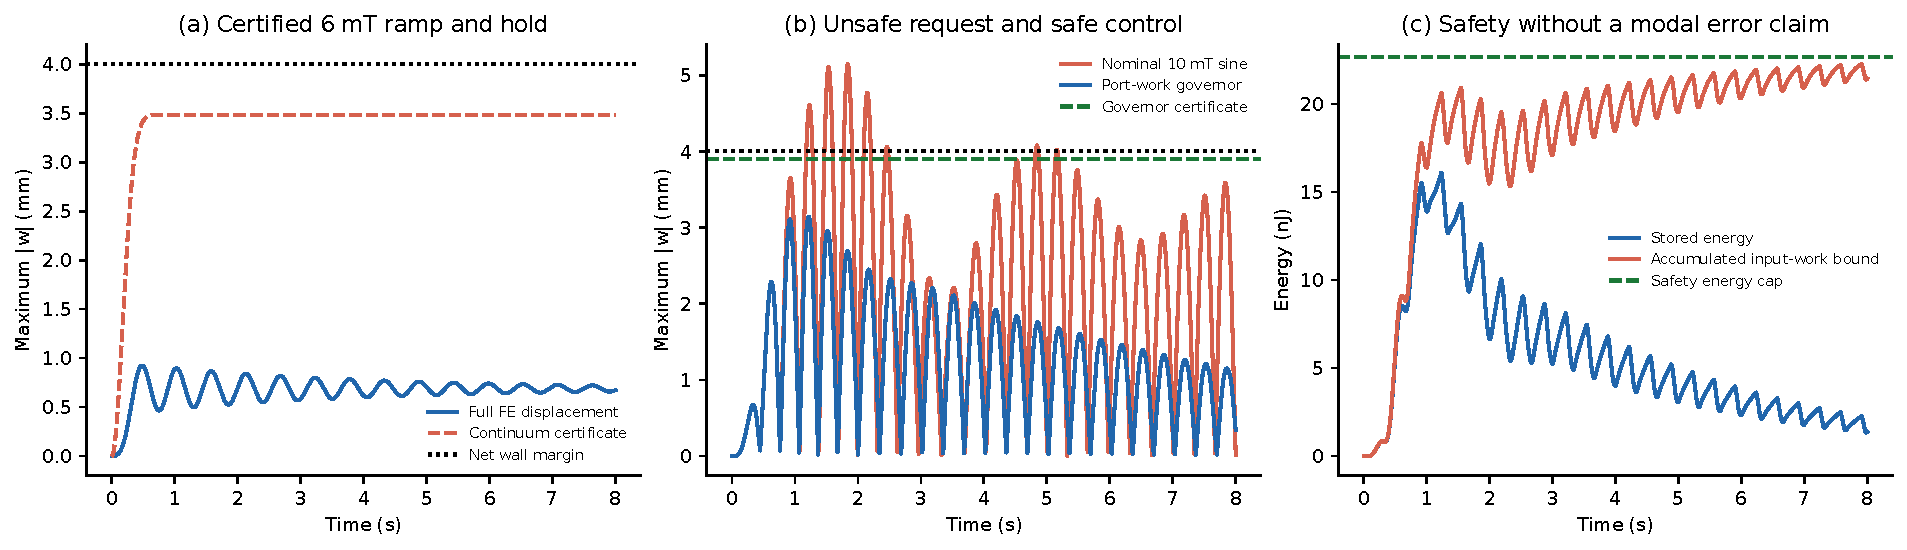
\includegraphics[width=\textwidth]{figures/unified_beam_safety_3panel.pdf}
\caption{Whole-beam safety for the shared full FE plant, with zero initial
energy and default drag.  (a) A $6$ mT monotone ramp and its all-time
continuum energy certificate.  (b) The $10$ mT ramped sinusoidal request
at $9.444949$ rad/s violates the $4$ mm net corridor margin; the actual
port-work governor preserves it with an analytically guaranteed bound.
(c) Stored energy and accumulated input-work bound for the governed case.
The wall half-width is $4.6$ mm and rod radius $0.6$ mm.  These
geometric constraints define the simulated corridor; patient-specific
clearance requires a corresponding geometry and parameter model.}
\label{fig:unifiedsafety}
\end{figure*}

For the $6$ mT sinusoid, the maximum tip discrepancies of the
$2$-, $4$-, and $8$-mode reconstructions against the full $64$-mode FE
trajectory are $22.7168$, $5.9661$, and $1.5156$ $\mu$m, respectively
($0.73510\%$, $0.19306\%$, and $0.04904\%$ of the full-FE peak).
These are measured truncation errors for this input, not rigorous bounds
for all neglected modes or all trajectories.  The full-continuum energy
certificate does not substitute any of them for an unknown error constant.
An independent COMSOL HermitianBeam integration of the same $32$-element
consistent-mass model gives a default-sinusoid peak of $3.09032$ mm;
its largest tip difference from the present integration is $0.11835$
$\mu$m.  Tightening the COMSOL relative tolerance to $10^{-8}$ reduces
the largest tip difference to $0.02160$ $\mu$m.
Independent COMSOL runs also reproduce the $6$ mT monotone-ramp safe case
and $10$ mT sinusoidal violation: their peaks are $0.924046$ and
$5.144787$ mm, with maximum cross-solver tip discrepancies of $0.00663$
and $0.03489$ $\mu$m, respectively.
This cross-check concerns the same mathematical model and does
not calibrate material or actuation parameters against hardware.

The closed-loop governor was also implemented inside COMSOL, coupling a
global ODE for $W/E_{\max}$ to the nonlinear magnetic end moment.
This run used the generalized-$\alpha$ time integrator with
$\rho_\infty=0$, relative tolerance $10^{-5}$, and a maximum internal
step of $0.002$ s; the $2001$ saved outputs are spaced by $0.004$ s.
Its full-FE centerline peak is $3.143643$ mm, leaving a sampled net
clearance of $0.856357$ mm.  The maximum tip discrepancy from the refined
Python trajectory is $0.582073$ $\mu$m, or $0.018516\%$ of its peak.
The applied field remains below $9.816986$ mT.  The COMSOL-integrated
work observer peaks at $22.253032$ nJ, or $0.9818823E_{\max}$;
$E\leq W\leq E_{\max}$ and the magnetic-power projection hold at every
saved time.  Its maximum work-observer discrepancy from Python is
$2.263\times10^{-12}$ J.

For an independent energy ledger, reconstruct $E$ from all displacement
and velocity DOFs and compute
\begin{align*}
 D_h(t)&=\int_0^t\alpha\dot q^{\mathsf T}M\dot q\dd\tau,\\
 R_E(t)&=E(t)-E(0)-[W(t)-W(0)]\\
       &\quad+D_h(t).
\end{align*}
Simpson quadrature on the saved outputs gives
$\max_t|R_E(t)|=5.796\times10^{-12}$ J after rounding up,
or $2.605\times10^{-4}$ of the work scale.
The Simpson--trapezoid difference for that dissipation integral is
$2.424\times10^{-13}$ J.  This COMSOL run uses high-frequency numerical
damping and a looser tolerance than the refined Python integration;
its ledger residual includes time-integration and output-quadrature
errors.  The separately integrated COMSOL work state is used for the
observer comparison, rather than replacing it by a coarse-output input
power integral.  These numerical checks corroborate the implementation;
the continuous-time clearance statement remains the analytic invariant
in Proposition~\ref{prop:unifiedgovernor}.

\begin{figure*}[t]
\centering
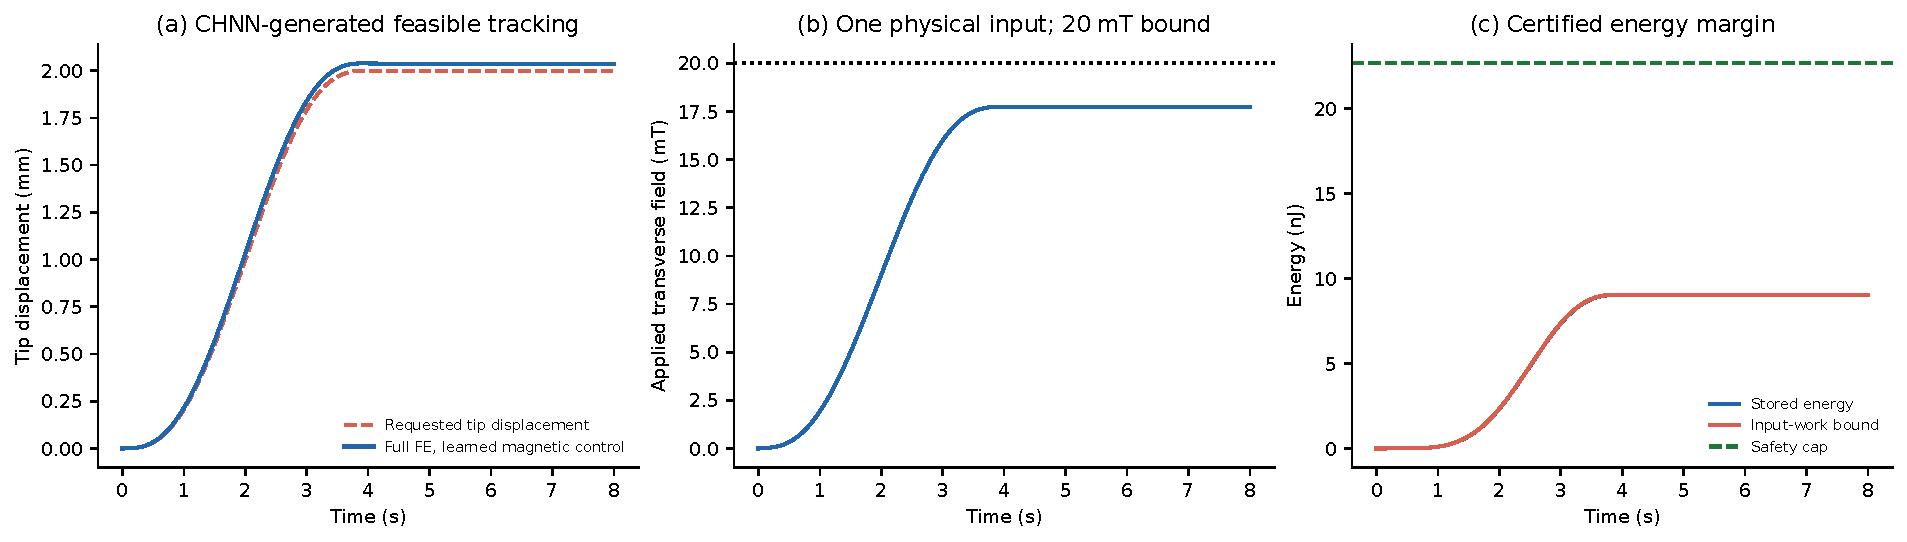
\includegraphics[width=\textwidth]{figures/unified_beam_learned_tracking.pdf}
\caption{The fitted GC17 CHNN and identified drag generate a single
bounded transverse magnetic input for the same full $32$-element FE beam.
(a) A feasible $2$ mm tip request over $4$ s and the actual full-FE tip
motion.  (b) The applied field remains below the declared $20$ mT limit.
(c) Stored energy and the actual-port work observer stay below the safety
cap.  The controller uses the exact first-two-mode projection available in
this simulation; the safety observer uses full-model tip power.
No modal actuation authority or unmeasured-state observer is assumed.
The governor is inactive for this feasible tracking request; its active
effect is tested separately in Figure~\ref{fig:unifiedsafety}.}
\label{fig:unifiedlearnedtracking}
\end{figure*}

\subsection{The learned CHNN generates a feasible magnetic tracking request}
\label{sec:unifiedlearnedcontrol}
To evaluate learned magnetic tracking, the fitted GC model
with seed $17$ and its identified dissipation coefficient generate a nominal
magnetic field for the full FE plant.  Let $z=(X_1,X_2,Y_1,Y_2)$ denote
the observed projection onto the first two static-field modes,
$\ell^{\mathsf T}X$ its reconstructed tip displacement, and
$h_\theta$ the fitted energy, including all learned mixed and
momentum-dependent quartic coefficients.  Define, in the dimensionless
time $\tau=\omega_0t$,
\begin{align}
 y&=\ell^{\mathsf T}X,\qquad
 y'=\ell^{\mathsf T}h_{\theta,Y},\\
 f_0&=\ell^{\mathsf T}h_{\theta,YX}h_{\theta,Y}\notag\\
 &\quad-\ell^{\mathsf T}h_{\theta,YY}
       (h_{\theta,X}+D_\theta h_{\theta,Y}),\\
 g_0&=\ell^{\mathsf T}h_{\theta,YY}d\cos(d^{\mathsf T}X),\\
 D_\theta&=\widehat\gamma\,\diag(\nu)^{-1}.
 \label{eq:unifiedlearnedoutput}
\end{align}
Where $g_0\ne0$, the nominal request is
\begin{align}
 a_r&=r''-k_p(y-r)-k_d(y'-r'),\\
 u_*&=(a_r-f_0)/g_0,\\
 B_{\mathrm{req}}&=B_0\operatorname{clip}_{[-b,b]}(u_*),\\
 b&=B_{\max}/B_0.
 \label{eq:unifiedlearnednominal}
\end{align}
The primes on $r$ denote derivatives in $\tau$.  We use
$k_p=16/\omega_0^2$, $k_d=8/\omega_0$, and
$\widehat\gamma=0.0486617964$.  Both Hessian blocks are evaluated from
the fitted model; they are not replaced by their quadratic-prior values.
The plant receives only the scalar $B_y$ through its actual tip moment,
after the work-governor projection.  It receives no independently
assigned modal forces.

The requested SI tip trajectory is
$y_{\mathrm{ref}}(t)=2\,\mathrm{mm}\,(10s^3-15s^4+6s^5)$ for
$s=t/(4\,\mathrm{s})\in[0,1]$, followed by a hold through $8$ s, and
$r(\tau)=y_{\mathrm{ref}}(\tau/\omega_0)$.
The field limit is $B_{\max}=20$ mT for this separate tracking protocol.
This limit follows from the static input authority: a $2$ mm
equilibrium requires $\vartheta=2y_{\mathrm{tip}}/L=0.05$ and
\begin{equation}
 B_y^{\mathrm{eq}}=
 \frac{EI\vartheta/(\mu L)+B_0\sin\vartheta}{\cos\vartheta}
 \simeq17.43\ \mathrm{mT}.
 \label{eq:unifiedstaticreach}
\end{equation}
The $10$ mT sinusoidal safety tests and the $2$ mm tracking experiment
thus use different input amplitudes, with the tracking limit set by the
required equilibrium field.

On the full $64$-DOF plant, the actual tip has an RMS tracking error of
$33.734$ $\mu$m and a maximum error of $47.069$ $\mu$m.  The final tip
position is $2.03515$ mm and the largest centerline displacement is
$2.03838$ mm.  The applied field peaks at $17.75695$ mT; saturation and
governor intervention occur at $0\%$ of saved times.  Thus the feasible
learned request passes through the filter unchanged, and the separate
unfiltered run is identical.  The input-work bound peaks at $9.05293$ nJ,
below the $22.66365$ nJ cap, and the same continuous-time safety invariant
applies.  The minimum absolute input gain along this run is
$0.0138678$ m, so the division in \eqref{eq:unifiedlearnednominal} does
not approach a singularity.  The physical power-balance residual is
$3.53\times10^{-20}$ J. This tracking result assumes access to the
two-mode projection of the full state. Extending it to incomplete sensing
requires a state observer and a corresponding tracking analysis.



A second run uses the CHNN identified by integral fitting of full-FE
COMSOL displacement and velocity exports, with
cosine multiplier $1.0223248822$. Its complete gradient and Hessian,
including learned momentum quartics, generate the same $2$ mm request
on the same full-FE Python plant. For this conservative fit, a separate
PSD drag identification on the existing Python-generated damped beam
trajectories gives $\widehat\gamma=0.0486617702$; this dissipative
training source is distinct from the COMSOL conservative data.
The tip RMSE is $33.726$ $\mu$m, its maximum error is $47.065$ $\mu$m,
and the largest centerline displacement is $2.038365$ mm.
The applied field peaks at $17.756854$ mT and the work observer at
$9.052842$ nJ. Saturation and governor intervention are again zero at
the saved times, and the physical power-balance residual is
$3.53\times10^{-20}$ J. This COMSOL-trained model and the Python-trained
GC17 model use the same physical plant.
The full-state projection and actual-port measurement assumptions are
unchanged, and the same continuum clearance guarantee applies.

Finally, the single uniform-field dipole supplies one boundary moment.
In static equilibrium with no distributed transverse loading,
$w_{ssss}=0$ and the free-tip shear condition imply
$w(s)=\vartheta s^2/(2L)$.
This one-parameter family cannot realize an arbitrary S-shaped static centerline.
The moving-base endpoint task in Section~\ref{sec:s-path} instead follows an
S-shaped tip history using axial base feed and magnetic bending.
The governor preserves the corridor for feasible magnetic requests.
Prescribing more general static shapes requires additional actuation
authority, such as distributed magnetic moments or independently
controlled loads.

\subsection{Finite initialization and port-error tolerances}
\label{sec:operational-tolerances}

The transverse action half-width $10^{-220}$ in
Appendix~\ref{app:measure-proof} quantifies local invariant-torus measure.
For operation, we instead construct a finite energy set and a robust
input-work constraint on the same full beam. This construction accepts
an ordinary finite-precision initial state, explicit sensing errors and
bounded command errors. It preserves clearance when the safety filter
changes the KAM-realizing request; exact quasiperiodic motion is then no
longer asserted.

\paragraph{Physical object and a measurable initialization set.}
For this calculation the mathematical plant is the frozen, symmetric
nodal $64\times64$ matrices $M,K$ supplied with the independent FE
comparison. All of their exported binary entries are treated as exact.
This retains the complete physical energy
\begin{equation}
 \begin{aligned}
 E(q,v)&=\tfrac12v^{\mathsf T}Mv+\tfrac12q^{\mathsf T}Kq
                 +E_0(1-\cos\vartheta),\\
 \dot E&=-\alpha v^{\mathsf T}Mv
          +Fv_w+\mu B\cos\vartheta\,v_\vartheta,
 \end{aligned}
 \label{eq:operational-physical-power}
\end{equation}
where $v=\dot q$, $\vartheta=e_\vartheta^{\mathsf T}q$,
$v_w=e_w^{\mathsf T}v$, $v_\vartheta=e_\vartheta^{\mathsf T}v$,
$E_0=\mu B_0$, and $F,B$ are the actual transverse tip force and field.
The same two physical ports appear in
\eqref{eq:physical-gradient-command}. The use of nodal matrices here
includes their small diagonalization discrepancy relative to the frozen
modal plant in Theorem~\ref{thm:full-fe-kam-lift}; no exact conjugacy between
these two finite-precision definitions is required for the work bound.

Let $b_r$ list the four cubic Bernstein control rows on every Hermite
element, including the fixed zero base coordinates, and define
\begin{equation}
 C_w=\max_r b_rK^{-1}b_r^{\mathsf T},\qquad
 E_c=\frac{c^2}{2C_w},\qquad c=4\,\mathrm{mm}.
 \label{eq:operational-fe-compliance}
\end{equation}
The Bernstein convex-hull property and Cauchy--Schwarz in the $K$ metric
give $\sup_s|w(s)|\leq\sqrt{2C_wE}$ for every FE state, including all
higher modes. Thus $E<E_c$ is a whole-centreline clearance condition.
Using exact Hermite coefficients $\ell/3=1/1200$ m, $256$-bit ball
matrix inverses and positive LDL pivots gives
$C_w<335.338810137\,\mathrm{m\,N^{-1}}$ and
$E_c>23.85646921\,\mathrm{nJ}$. This discrete certificate agrees with
the continuum compliance while avoiding an unbudgeted matrix-rounding step.

Set $K_b=K+E_0e_\vartheta e_\vartheta^{\mathsf T}$ and
\begin{equation}
 Q(q,v)=\tfrac12v^{\mathsf T}Mv+\tfrac12q^{\mathsf T}K_bq.
 \label{eq:operational-initial-metric}
\end{equation}
For full-state estimates $(\widehat q,\widehat v)$, require the initialization
error to satisfy $Q(q-\widehat q,v-\widehat v)\leq\mathcal E_{\rm init}$.
Since $1-\cos\vartheta\leq\vartheta^2/2$ and $\sqrt Q$ is a norm,
\begin{equation}
 E(q,v)\leq Q(q,v)\leq\overline E_0
 :=\left[\sqrt{Q(\widehat q,\widehat v)}
                  +\sqrt{\mathcal E_{\rm init}}\right]^2.
 \label{eq:operational-initial-energy}
\end{equation}
This specifies a nonzero finite-dimensional admissible initialization
region with nonempty interior, without deciding membership in an exact
invariant torus.
The energy-error bound is a full-state condition; tip sensing alone does
not bound unobserved bending or kinetic energy.

\paragraph{Sensing and execution error envelopes.}
Let $u=(u_F,u_B)$ be the commanded ports and suppose that, throughout the
specified interval,
\begin{equation}
 \begin{aligned}
 F&=(1+g_F)u_F+e_F,\\
 B&=(1+g_B)u_B+e_B,\\
 |g_i|&\leq\eta_i,\qquad |e_i|\leq\epsilon_i.
 \end{aligned}
 \label{eq:operational-actuator-envelope}
\end{equation}
Assume available estimates obey
$|v_w-\widehat v_w|\leq\delta_v$,
$|\vartheta-\widehat\vartheta|\leq\delta_\vartheta$ and
$|v_\vartheta-\widehat v_\vartheta|\leq\delta_\omega$.
Define the estimated power coefficients and their error bounds by
\begin{equation}
 \begin{aligned}
 \widehat a_F&=\widehat v_w,&\Delta_F&=\delta_v,\\
 \widehat a_B&=\mu\cos\widehat\vartheta\,\widehat v_\vartheta,
 &\Delta_B&=\mu(\delta_\omega+
                         |\widehat v_\vartheta|\delta_\vartheta).
 \end{aligned}
 \label{eq:operational-port-estimation}
\end{equation}
The cosine is one-Lipschitz on the real line, hence $|a_i-\widehat a_i|
\leq\Delta_i$. Both sensing error and relative execution error are covered
by the convex, positively homogeneous function
\begin{equation}
 P^+(u)=\sum_{i\in\{F,B\}}
 \left\{\widehat a_i u_i+
 [\Delta_i+\eta_i(|\widehat a_i|+\Delta_i)]|u_i|\right\}.
 \label{eq:operational-robust-power}
\end{equation}
In particular, $P^+(0)=0$. There is no division by a measured velocity,
so a zero or incorrectly signed noisy velocity creates no singularity.

The independent additive errors need a separate energy allowance.
For $\alpha>0$, write $m_F=e_w^{\mathsf T}M^{-1}e_w$ and
$m_\vartheta=e_\vartheta^{\mathsf T}M^{-1}e_\vartheta$, and put
\begin{equation}
 p_e=\frac{(\epsilon_F\sqrt{m_F}
                    +\mu\epsilon_B\sqrt{m_\vartheta})^2}{4\alpha},
 \qquad R_T=Tp_e.
 \label{eq:operational-additive-reserve}
\end{equation}
For time-dependent bounds one may instead integrate their corresponding
$p_e(t)$. With $r=e_we_F+\mu e_\vartheta e_B\cos\vartheta$, completion of
the square gives
\begin{equation}
 r^{\mathsf T}v-\alpha v^{\mathsf T}Mv
 \leq\frac{r^{\mathsf T}M^{-1}r}{4\alpha}\leq p_e.
 \label{eq:operational-damping-reserve-proof}
\end{equation}
All quantities in these equations use SI units: $P^+,p_e$ are powers,
and $Q,E,R_T$ are energies. No dissipated energy needs to be measured.

\begin{proposition}[Robust finite-horizon work and clearance]
\label{prop:operational-robust-work}
Fix $T>0$ and $\overline E_0<C:=E_{\max}-R_T<E_c-R_T$.
Initialize $W(0)=\overline E_0$ and integrate $\dot W=P^+(u)$.
Clip a requested force and field to symmetric command limits, then apply
$u=\sigma u_{\rm req}$, with $\sigma=1$ if
$P^+(u_{\rm req})\leq\kappa(C-W)$, and otherwise
\begin{equation}
 \sigma=\frac{\kappa(C-W)}{P^+(u_{\rm req})},\qquad \kappa>0.
 \label{eq:operational-radial-governor}
\end{equation}
For solutions satisfying the mechanical power identity and the stated
error envelopes, throughout $0\leq t\leq T$,
\begin{equation}
 \begin{aligned}
 E(t)&\leq W(t)+tp_e\leq C+R_T=E_{\max},\\
 \sup_s|w(s,t)|&\leq\sqrt{2C_wE_{\max}}<c.
 \end{aligned}
 \label{eq:operational-robust-clearance}
\end{equation}
Zero command remains feasible, even with nonzero sensing errors. To enforce
actual actuator limits $F_{\lim},B_{\lim}$, use command limits
$(F_{\lim}-\epsilon_F)/(1+\eta_F)$ and
$(B_{\lim}-\epsilon_B)/(1+\eta_B)$, respectively.
\end{proposition}
\begin{proof}
The two non-additive port powers are at most $P^+(u)$, by
\eqref{eq:operational-port-estimation} and
\eqref{eq:operational-actuator-envelope}. Equation
\eqref{eq:operational-damping-reserve-proof} bounds the remaining power
and damping together. Thus $\dot E\leq\dot W+p_e$, and integration with
\eqref{eq:operational-initial-energy} proves $E\leq W+tp_e$.
Positive homogeneity makes the radial choice satisfy
$\dot W\leq\kappa(C-W)$; consequently
$C-W(t)\geq(C-W(0))e^{-\kappa t}>0$.
The spatial compliance bound completes the proof. The amplitude limits
follow directly from $|F|\leq(1+\eta_F)|u_F|+\epsilon_F$ and its field
counterpart. If additive errors vanish, $R_T=0$ and the same argument
holds for all time and for any $\alpha\geq0$. A constant nonzero additive
error allowance has the stated finite horizon; it is not an all-time KAM
or clearance assertion.
\end{proof}

\paragraph{Sampled sensing and delayed execution.}
The sensing bounds must cover the age of the data, not only sensor
quantization. For a sample at $t_k$ used for an interval of length $h_k$,
let the maximum age including sensing latency be $\ell_k$.
If valid bounds $|\dot v_w|\leq A_w$,
$|v_\vartheta|\leq V_\vartheta$ and
$|\dot v_\vartheta|\leq A_\vartheta$ hold on that interval, replace
\begin{equation}
 \delta_v\mapsto\delta_v+A_w\ell_k,\quad
 \delta_\vartheta\mapsto\delta_\vartheta+V_\vartheta\ell_k,\quad
 \delta_\omega\mapsto\delta_\omega+A_\vartheta\ell_k.
 \label{eq:operational-sensor-age}
\end{equation}
Compute $P_k^+$ with this interval envelope. A fully discrete sufficient
rule is to hold $u_k$ such that
$h_kP_k^+(u_k)\leq C-W_k$ and set
$W_{k+1}=W_k+h_kP_k^+(u_k)$. Linear interpolation of $W$ proves the same
within-interval energy bound; $u_k=0$ remains feasible. This rule does
not treat a value at one sample as an interval guarantee.

Similarly, if a continuously specified command has a verified slew bound
$|\dot u_i|\leq S_i$ and the applied copy is delayed by at most $d_i$,
including a zero-order-hold age when applicable, it suffices to use
\begin{equation}
 \epsilon_i\geq\epsilon_{i,0}+(1+\eta_i)S_id_i
 \label{eq:operational-execution-age}
\end{equation}
in the additive reserve. This is an explicit joint delay/slew budget.
The radial governor alone does not impose a slew limit. A controller
that also enforces slew must verify its feasibility, or use the discrete
interval-power rule above. The numerical experiment below uses continuous
bounded port estimates and the declared direct execution-error envelope;
it does not identify a hardware latency or an unmeasured acceleration bound.

\paragraph{A nonzero SI budget next to the finite-amplitude reference.}
The reference $(\widehat q,\widehat v)$ is the frozen nodal reconstruction
of phase $(0,0)$ of the computed Fourier candidate for the integral-COMSOL
fit, with the learned velocity $h_Y$, rather than an assumed exact torus
point. Its quadratic energy is below $21.45855219$ nJ.
For $\mathcal E_{\rm init}=5$ pJ, ball evaluation of
\eqref{eq:operational-initial-energy} gives
$\overline E_0<22.11866366$ nJ. This full-state ellipsoid implies, among
other coordinate bounds, an initial tip-displacement error below
$56.006$ $\mu$m and tip-angle error below $1.19851$ mrad.
It also implies mass-weighted RMS velocity error below $0.316981$ mm/s,
where the squared RMS is $\delta v^{\mathsf T}M\delta v/(\rho A_cL)$.
These are projections of one energy ellipsoid; their endpoints cannot
be independently combined as a Cartesian error box.

\begin{table}[t]
\centering\small
\caption{One sufficient operational budget for the full nodal FE plant.
Bounds are deterministic hypotheses; they are not measured sensor specifications.}
\label{tab:operational-tolerances}
\setlength{\tabcolsep}{3pt}
\begin{tabular}{lr}
\hline
Quantity & Value or outward bound\\
\hline
Horizon $T$ & $4$ s\\
Energy cap $E_{\max}$ & $22.66$ nJ\\
Initialization error $\mathcal E_{\rm init}$ & $5$ pJ\\
Angle / angular-rate error & $1$ mrad / $0.01$ rad/s\\
Tip-velocity error & $0.1$ mm/s\\
Relative force and field execution error & $1\%$ each\\
Additive force / field error & $0.5$ nN / $0.05$ $\mu$T\\
Additive work reserve $R_T$ & $<0.09677917$ nJ\\
Available commanded-work cap $C$ & $>22.56322083$ nJ\\
Initial commanded-work margin & $>0.44455717$ nJ\\
Whole-centreline displacement bound & $<3.898405$ mm\\
Minimum net wall clearance & $>0.101595$ mm\\
\hline
\end{tabular}
\end{table}
The declared actual limits are $20$ mT and $20$ $\mu$N; the latter
corresponds to a gradient norm $1$ T/m in the ideal local magnetic
realization. The command bounds reserve the relative and additive errors
before clipping. Matrix ball arithmetic, rather than a two-mode estimate
of unobserved velocity, gives $m_F<4.452635925\,10^6$ and
$m_\vartheta<3.940922387\,10^{13}$ in their respective SI inverse-mass
units, which establish the work reserve in the table.

\paragraph{Full-model numerical check.}
The reproducibility directory
\texttt{reviewer\_revision\_20261008/robustness} contains the complete
input matrices, learned coefficients, finite initial reference, original-file
hashes, code and trajectories. The physical integrator retains
$\Phi^{\mathsf T}M\Phi$ and $\Phi^{\mathsf T}K_b\Phi$ in full, so it
integrates the frozen nodal plant in a well-scaled modal basis instead of
discarding diagonalization residuals. The requesting controller uses the
same fitted $h_Y,h_{YX},h_{YY}$ and velocity-to-momentum inverse as
\eqref{eq:full-fe-hamiltonian-feedback}, with an additional bounded
low-state perturbation. Independent deterministic sinusoids supply the
stated port-sensor, gain and additive execution errors. The full-state
initialization error is verified by direct Arb matrix products, including
the modal-to-nodal transformation.

The initialized energy is $21.743724$ nJ, with a $46.354$ $\mu$m tip
position error and a $0.347654$ mm/s tip velocity error; its combined
initial error energy is below $4.951$ pJ. Over $4$ s the saved-time
Bernstein centreline bound is below $1.944145$ mm and the physical
energy is below $21.744899$ nJ. The work filter is active at $97.8011\%$
of the $2001$ saved times, illustrating its conservative use of work
without crediting dissipated energy. Its activation changes the desired
Hamiltonian trajectory. Clearance follows from
Proposition~\ref{prop:operational-robust-work}, while invariant-torus
persistence remains the separate conservative and ideal-feedback result.

The Radau run uses relative tolerance $2\,10^{-8}$ and componentwise
absolute tolerances $2\,10^{-13}$ for modal positions,
$2\,10^{-11}$ for modal velocities and $2\,10^{-13}$ for normalized
energy states. Simultaneously reducing them tenfold changes the saved tip
trajectory by less than $0.010$ $\mu$m and the energy by less than
$3.2\,10^{-15}$ J; the refined energy-ledger residual is below
$3\,10^{-16}$ J. These are numerical implementation checks, not a
validated enclosure of the integrated trajectory. The continuous-time
clearance statement uses the analytic work proof and its independently
validated initialization and parameter bounds.

\subsection{A physically actuated S-shaped endpoint path}
\label{sec:s-path}
The moving clamped base permitted by the distributed formulation supplies
an axial feed coordinate $b(t)$, while the same single transverse magnetic
field bends the catheter. In the Cartesian small-slope model,
the centreline is
\begin{equation}
 \begin{aligned}
 r(s,t)&=\bigl(b(t)+s,w(s,t)\bigr),\\
 r_{\rm tip}(t)&=\bigl(b(t)+L,w(L,t)\bigr).
 \end{aligned}
 \label{eq:s-path-geometry}
\end{equation}
The axial feed and magnetic bending together prescribe the endpoint
history. The material length remains
$80$ mm throughout; advancing a varying length through a guide is a
different boundary-value problem.

The base starts at rest. Over the first second its speed is
$\dot b=v_b(10\xi^3-15\xi^4+6\xi^5)$, where $\xi=t/(1\,\mathrm{s})$
and $v_b=4\,\mathrm{mm\,s^{-1}}$; afterwards $\dot b=v_b$.
The transverse request is zero until $2$ s. During the subsequent
$12$ s stroke, put $\sigma=(t-2\,\mathrm{s})/(12\,\mathrm{s})$ and prescribe
\begin{equation}
 y_r(t)=\frac{8A}{3\sqrt3}
       \left(\frac12\sin 2\pi\sigma-\frac14\sin4\pi\sigma\right),
 \quad A=1.5\,\mathrm{mm}.
 \label{eq:s-path-reference}
\end{equation}
Outside this interval $y_r=0$. Its position, velocity and acceleration
join continuously to zero, and its two lateral extrema are $\pm A$.
The resulting S-shaped endpoint stroke advances $48$ mm axially.
The base acceleration is at most $7.5\,\mathrm{mm\,s^{-2}}$ and ends
before any bending command is applied. Consequently the beam is exactly
straight during axial acceleration and the base has zero acceleration
throughout the bending stroke. There is no axial fluid load, guide friction,
or imposed axial prestress in this test.

\paragraph{Base work and clearance.}
Let $m_b=\rho A_cL$ denote the rod mass, with $A_c$ its cross-sectional area.
Orthogonality of the axial and transverse Cartesian velocities gives
\begin{equation}
 E_{\rm total}=E_\perp+\frac12m_b\dot b^2,
 \qquad P_b=F_b\dot b=m_b\ddot b\dot b.
 \label{eq:s-path-base-energy}
\end{equation}
Here $E_\perp$ is the same transverse kinetic, bending and static-field
energy used in the clearance theorem. The chosen timing also avoids
transverse geometric-stiffness effects from an accelerating bent beam:
the axial inertial load acts only while $w=0$. During bending, axial
translation is force-free in the stated model. Thus
\begin{equation}
 \dot E_{\rm total}
 =\mu B_y\cos\vartheta\,\dot\vartheta
  -\alpha\dot q^{\mathsf T}M\dot q+P_b.
 \label{eq:s-path-total-power}
\end{equation}
The base work is $W_b=m_b\dot b^2/2$ and is accounted for separately
from the magnetic input budget.
The straight, open-ended corridor is invariant under axial translation.
Its lateral noncollision proof therefore applies to $E_\perp$ and the
actual magnetic port, while the separate base-energy balance is retained.
For the same $4$ mm net clearance and $0.95E_c$ transverse work cap,
the continuous-time centreline bound remains $3.898718$ mm.
This statement would require additional work and geometry terms for
curved walls, axial contact, variable insertion length or axial drag.

\paragraph{Learned control and comparisons.}
The conservative readout is the integral fit to full-FE COMSOL
position--velocity data in Section~\ref{sec:comsol-identification}.
It has cosine multiplier $1.0223248822$ and includes all fitted quartic
terms; its invariant torus is certified independently. The conservative
coefficients and the nonnegative drag readout are held fixed throughout
this experiment. The controller evaluates its drift and
magnetic input gain from the complete learned gradient and Hessian,
as in the preceding tracking construction. For this experiment the
feedback error uses the actual full-beam tip position and velocity;
the first two modal projections supply the learned drift and gain.
The request is clipped to $|B_y|\leq20$ mT and passed through the
same physical input-work governor. Every plant run integrates all
$64$ FE degrees of freedom. The imposed base motion has the same
force and speed budget in every comparison.

\begin{table*}[t]
\centering\small
\caption{S-path tracking on the full FE plant. RMS errors use the 12 s
stroke; maxima use the full 16 s simulation. All baselines share the
same trajectory, physical input and field bound.}
\label{tab:s-path}
\begin{tabular}{lrr}
\hline
Controller & RMS ($\mu$m) & Max. ($\mu$m)\\
\hline
CHNN, measured tip feedback & 6.419 & 12.907\\
Quadratic model, measured tip feedback & 6.207 & 12.476\\
Known-physics static inverse feedforward & 4.124 & 8.005\\
CHNN, modal-output feedback & 25.308 & 41.544\\
\hline
\end{tabular}
\end{table*}

The known-physics static inverse has the smallest tracking error in
Table~\ref{tab:s-path} for this slow, weakly nonlinear nominal trajectory.
The learned controller also follows the S-shaped endpoint path, with
accuracy depending on the measured output: full-tip feedback reduces
the CHNN error relative to its two-mode reconstruction while using
the same fitted energy and physical input.

The learned controller uses a peak field of $12.9177$ mT and a sampled
peak field slew of $10.4268\,\mathrm{mT\,s^{-1}}$. Its largest
centreline displacement is $1.48892$ mm, leaving $2.51108$ mm of
net lateral clearance at the saved times; the largest slope is
$0.03718$ rad. The recorded work-based energy estimate peaks at $4.84997$ nJ,
below the $22.66365$ nJ cap, and neither field saturation nor governor
intervention occurs. The base's maximum kinetic energy is $0.796205$ nJ,
its peak ideal inertial force is $0.746442\,\mu$N, and its peak power
is $1.90256$ nW. Numerical total-energy balance includes this base work
and has maximum residual $2.44\times10^{-18}$ J.
Tightening integration tolerances by a factor of ten and halving the
maximum step changes the tip by at most $3.14\times10^{-12}$ m and
the commanded field by at most $1.47\times10^{-10}$ T at saved times.

\paragraph{Independent COMSOL field replay.}
An additional COMSOL solve integrates the same full beam for $16$ s
using the saved learned-controller field, with piecewise-cubic field
interpolation, generalized-alpha integration, relative tolerance
$10^{-8}$ and maximum step $0.002$ s. The prescribed field is the
controller output from the preceding simulation. Its tip differs from the
Python result by $1.312\times10^{-10}$ m RMS and at most
$4.038\times10^{-10}$ m, and its S-stroke tracking RMSE is
$6.419\,\mu$m. COMSOL independently integrates the mechanical
response to this prescribed command; the controller is not recomputed
online in this replay. Axial translation is reconstructed using the same analytic
base protocol. Power balance reconstructed by trapezoidal integration
of the $0.004$ s output samples has a $1.244\times10^{-14}$ J residual;
this diagnostic is distinguished from the much tighter internal Python
work-state integration and is not used as a rigorous solver-error bound.

\begin{figure*}[t]
\centering
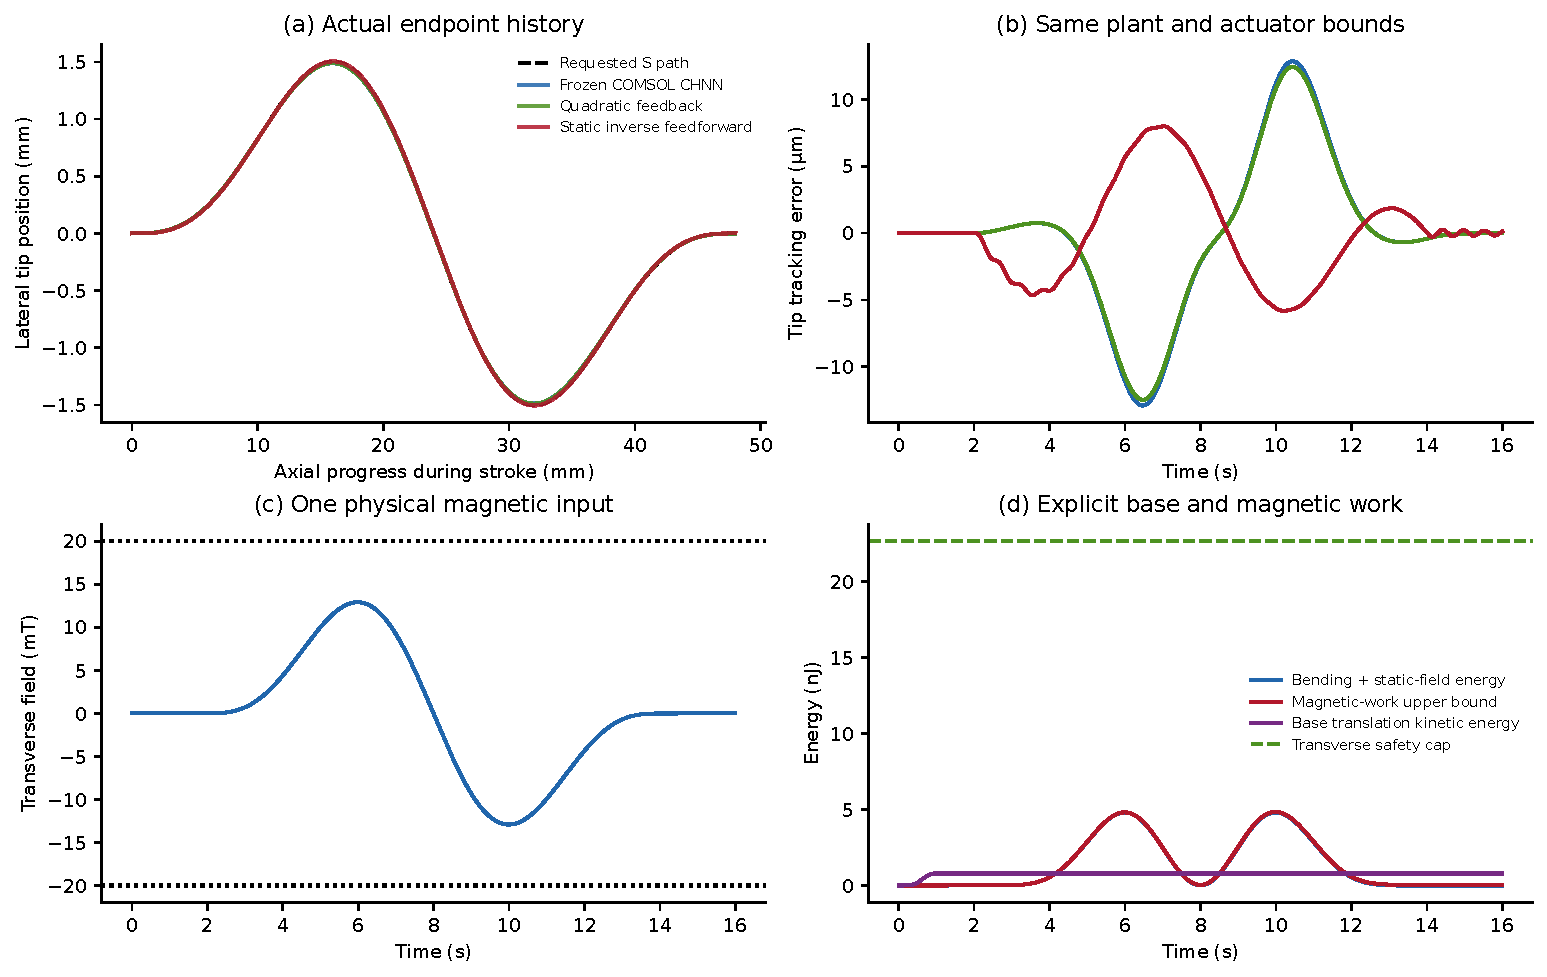
\includegraphics[width=\textwidth]{figures/fig_s_path_tracking.pdf}
\caption{A realized S-shaped endpoint path generated by axial base feed
and one transverse magnetic input. The controller uses the fitted
COMSOL-trained CHNN on the full FE plant. Axial translation work is
explicitly included in the energy balance. The matched controls reveal
that known-physics static inverse feedforward is more accurate on this
particular slow nominal path.}
\label{fig:s-path}
\end{figure*}


\section{Structure-preserving time integration}
\label{app:integrator}
For a real smooth Hamiltonian, implicit midpoint is
\begin{equation}
 x_{k+1}=x_k+hJ\nabla H\big((x_k+x_{k+1})/2\big).
\end{equation}
Let $A=JH''(\bar x)$. Differentiation gives $D\Phi_h=(I-hA/2)^{-1}(I+hA/2)$. Since $A^{\mathsf T}J+JA=0$, this Cayley transform satisfies $D\Phi_h^{\mathsf T}JD\Phi_h=J$ whenever the implicit equation defines a differentiable local map. The proof assumes the nonlinear step is solved exactly; residual tolerances add a numerical defect. Explicit RK4 is not symplectic in general. For the separable physical Hamiltonian, the kick--drift--kick St\"ormer--Verlet map is also symplectic, because each substep is the exact flow of the kinetic or potential Hamiltonian. A general learned momentum-dependent quartic no longer admits that separable split, so the same formula cannot be reused without justification.

Energy error and symplecticity are distinct diagnostics. Finite-time energy plots are evaluated against the specified reference Hamiltonian and accompanied by a step-size check. A small integration error does not certify a Diophantine inequality, nor does a positive finite-time Lyapunov estimate alone establish asymptotic chaos. These facts determine the labels used in the numerical figures.

\section{The fourth-order central generating-function scheme}
\label{app:central4}
Let $f=J\nabla H$, $A=H''$ and define a central generating function
\begin{equation}
 S_h(x)=hH(x)+\frac{h^3}{24}f(x)^{\mathsf T}A(x)f(x).
\end{equation}
The map is specified implicitly by
\begin{equation}
 x_+-x_-=J\nabla S_h\big((x_-+x_+)/2\big).
 \label{eq:central4}
\end{equation}
The central generating-function construction and fourth-order formula are classical \citep[Theorem~24, p.~90; formula on p.~95]{feng}; geometric integration is developed systematically by \citet{hairer}. Here every derivative is
computed from the same learned scalar Hamiltonian. The identity
\begin{equation}
 J\nabla(f^{\mathsf T}Af)=f''[f,f]-2(f')^2f
\end{equation}
follows by differentiating both occurrences of $f$, using $f'=JA$ and
$J^{\mathsf T}=-J$. It gives the displacement implemented in the
reproducibility code:
\begin{equation}
 g_h=hf+\frac{h^3}{24}\bigl(f''[f,f]-2(f')^2f\bigr).
\end{equation}
The Hessian $S_h''$ is symmetric, so the midpoint Cayley-transform argument
in Supplement~\ref{app:integrator} proves exact symplecticity of the
locally defined map. Since $S_{-h}=-S_h$, interchanging its endpoints
proves reversibility.

To verify order, expand an exact orbit about its temporal midpoint $x_0$.
Its endpoint midpoint $m$ and endpoint difference satisfy
\begin{align}
 m&=x_0+\tfrac18h^2f'(x_0)f(x_0)+O(h^4),\\
 x_+-x_-&=hf(x_0)+\tfrac1{24}h^3
       \bigl(f''[f,f]+(f')^2f\bigr)(x_0)\nonumber\\
       &\quad+O(h^5).
\end{align}
Substituting $x_0=m-\tfrac18h^2f'(m)f(m)+O(h^4)$ gives
$x_+-x_-=g_h(m)+O(h^5)$, proving fourth order under the required
smoothness and local solvability assumptions.

\subsection{Integration accuracy for the learned magnetic energy}
\label{app:unified-integrator-check}
We implement \eqref{eq:central4} for the Python-trained GC17 Hamiltonian,
retaining its complete cosine and all mixed and momentum-dependent
quartics. Polynomial and trigonometric derivatives through order four
are evaluated analytically from the fitted energy; they supply both the
central displacement and its Newton Jacobian. This test closes all
forcing and damping ports. Starting at $(X_1,X_2,Y_1,Y_2)=(0.1,0.06,0,0.02)$,
we integrate to $\tau=10$ and compare against DOP853 with relative and
absolute tolerances $3\times10^{-14}$ and $3\times10^{-16}$.
Tightening the reference tolerances from $2\times10^{-13}$ and
$2\times10^{-15}$ changes the sampled reference by at most
$8.32\times10^{-14}$ per state component.
The endpoint errors in Table~\ref{tab:unified-integrator-check} approach
fourth order for Central4 and second order for implicit midpoint.

\begin{table}[htbp]
\centering\small
\setlength{\tabcolsep}{2.5pt}
\caption{Conservative integration of the GC17 energy.
Errors are Euclidean endpoint errors in the balanced dimensionless state;
orders compare successive step halvings.}
\label{tab:unified-integrator-check}
\begin{tabular}{rrrrr}
\toprule
$h$ & Midpoint error & Order & Central4 error & Order\\
\midrule
$0.08$ & $7.1351\times10^{-2}$ & --- & $1.8346\times10^{-3}$ & ---\\
$0.04$ & $1.9383\times10^{-2}$ & $1.8802$ & $1.1784\times10^{-4}$ & $3.9606$\\
$0.02$ & $4.8966\times10^{-3}$ & $1.9849$ & $7.4149\times10^{-6}$ & $3.9902$\\
$0.01$ & $1.2265\times10^{-3}$ & $1.9972$ & $4.6422\times10^{-7}$ & $3.9976$\\
\bottomrule
\end{tabular}
\end{table}

The largest implicit-step residual in the infinity norm is
$2.00\times10^{-15}$, with at most three Newton evaluations per step.
For each tested step size, differentiating the converged implicit equation
gives its one-step tangent map $D\Phi_h$. The largest measured defect
$\|D\Phi_h^{\mathsf T}JD\Phi_h-J\|_\infty$ is
$3.34\times10^{-16}$ for Central4 and $2.24\times10^{-16}$ for midpoint.
An independent fourth-order central-difference evaluation of the solved
step map agrees with the implicit tangent to $1.39\times10^{-12}$;
its largest symplectic defect is $2.75\times10^{-12}$.
Thus both methods preserve the symplectic structure to the measured
implicit-solve and arithmetic accuracy, while their convergence orders
differ. The test assesses numerical integration of the complete
momentum-dependent Hamiltonian; the KAM statement follows separately
from its analytic certificate.

\section{Complex-gradient descent with a strict descent margin}
\label{sec:complex-descent}

Theorem 3 in the published version of \citet{zhang} motivates complex-gradient optimization,
but a stationary-point conclusion requires a strict descent margin. The
following convention-explicit statement also applies to a smooth CHNN
regression objective.

\begin{proposition}[Complex descent]
Let $\mathcal L:\mathbb C^P\simeq\mathbb R^{2P}\to\mathbb R$ be bounded
below and have an $L$-Lipschitz real gradient on every segment traversed by
the iterates. For $w=a+ib$, define
$G(w)=\nabla_a\mathcal L+i\nabla_b\mathcal L
=2\partial\mathcal L/\partial\bar w$.
Choose a constant $\rho\in\mathbb C$ with
$\kappa=\operatorname{Re}\rho-(L/2)|\rho|^2>0$, and update
$w_{t+1}=w_t-\rho G(w_t)$.
Then
\[
 \mathcal L(w_{t+1})\leq\mathcal L(w_t)-\kappa\|G(w_t)\|_2^2,
 \qquad \lim_{t\to\infty}\|G(w_t)\|_2=0,
\]
and
\[
 \min_{0\leq t<T}\|G(w_t)\|_2^2
 \leq\frac{\mathcal L(w_0)-\inf\mathcal L}{\kappa T}.
\]
\end{proposition}

\begin{proof}
Under realification, multiplication by $\rho=u+iv$ is $uI+vJ_c$, with
$J_c^\top=-J_c$ and $J_c^\top J_c=I$.
Hence the update has inner product $-u\|G\|^2$ with the real gradient
and squared norm $|\rho|^2\|G\|^2$.
The real descent lemma gives the first inequality. Summing it and using
the lower bound for $\mathcal L$ gives
$\kappa\sum_{t\geq0}\|G(w_t)\|^2\leq\mathcal L(w_0)-\inf\mathcal L$.
Square summability proves convergence of the gradient norm and the minimum
bound. The result asserts convergence to stationarity in gradient norm,
not convergence to a global minimum or to a particular parameter vector.
\end{proof}

For a real step this condition is $0<\rho<2/L$ under the stated convention.
The case $\rho=0$, allowed by a non-strict printed step-size interval,
cannot imply gradient convergence. Nonsmooth complex activations also need
separate treatment; a smooth polynomial CHNN satisfies the differentiability
requirements, with a Lipschitz gradient bound on any bounded iterate region.
This proposition concerns smooth gradient descent; the experimental
readouts are fitted by linear least squares.

\section{An explicit local KAM measure estimate}
% Standalone appendix fragment; the root manuscript supplies the section heading.
% Literature keys: chierchia2021measure, biasco2018measure.
% All angular variables in this appendix have period 2*pi.
\label{app:measure-proof}
\subsection{A fixed-domain bound and its scope}
\label{sec:measure-fixed-tube}

This appendix quantifies a sufficient local measure bound for the
Hamiltonian identified from COMSOL integral observations. The construction
uses the exact finite-amplitude torus and bounds the complete transformed
Hamiltonian, including the action-domain remainder. The resulting width
illustrates the conservatism of the explicit constants in
\citet{chierchia2021measure}.

\begin{samepage}
\begin{theorem}[Explicit finite-amplitude tubular measure]
\label{thm:measure-finite-tube}
Let $h$ be the fitted Hamiltonian certified in
Section~\ref{sec:validated-integral-learning}, and let $K_\infty$ be its
exact invariant torus. There is an explicitly constructed analytic
symplectic chart $\Xi=\Psi\circ\Phi_{\chi}$, specified in
Sections~\ref{sec:measure-explicit-tube}--\ref{sec:measure-tube-normal-form},
that fixes this torus at zero action.
For the fixed domain
\begin{equation}
 U_w=\Xi\bigl(\mathbb T^2_{2\pi}\times(-w,w)^2\bigr),
 \qquad w=10^{-220},
 \label{eq:measure-fixed-tube}
\end{equation}
the KAM fraction satisfies
\begin{equation}
 f_{\rm KAM}(U_w)\geq0.9669383.
 \label{eq:measure-certified-fraction}
\end{equation}
The centre torus is the previously certified motion with the
$1.8977904$ mm tip witness and the $1.8977962$ mm all-phase centreline
bound. The width $w$ is a dimensionless action half-width, not a
displacement amplitude.
\end{theorem}
\end{samepage}

\begin{proof}
The explicit chart and a convergent quadratic normalization give
\[
 h\circ\Xi=e+\omega\cdot I+\tfrac12 I^\top\overline A I+R_3,
 \qquad \omega=2\pi\varpi.
\]
The outward bounds are
$\|\overline A\|_\infty\leq3$,
$\|\overline A^{-1}\|_\infty\leq5100$ and
$\|R_3\|_{2w,1/128}\leq4\times10^{51}w^3$.
Use the global KAM theorem with real action radius $w$, complex radius
$2w$, final angle strip $1/256$, frequency exponent $\tau=2$,
boundary allowance $\rho=w/500$ and
$\alpha=w/(1000\times5100)$.
The dimensionless smallness quantity is at most
$3.1212\times10^{-155}$, below the theorem threshold
$7.6577\times10^{-155}$.
The geometric estimate in Section~\ref{sec:measure-ck-bound} gives
\begin{equation}
 \begin{aligned}
 1-f_{\rm KAM}(U_w)
 &\leq\frac{25}{16}\left(
      \frac{4\rho}{w}+\frac{8\alpha L\zeta(2)}{w}\right)\\
 &=\frac{25}{16}\left(0.008+0.008\zeta(2)\right)
 <0.0330617,
 \end{aligned}
 \label{eq:measure-budget}
\end{equation}
where $L=5100$. The two terms account for the boundary layer and all
integer resonance strips, respectively. Symplecticity transfers this
relative measure to $U_w$ without a density correction.
\end{proof}

\begin{table}[t]
\centering\small
\caption{Outward bounds for the explicit finite-amplitude tube.
The smallness quotient is the tested perturbation divided by the
sufficient threshold; failure of that test does not imply chaos.}
\label{tab:measure-tube-certificate}
\begin{tabular}{lr}
\hline
Quantity & Bound or value\\
\hline
Initial chart action radius & $10^{-3}$\\
Quadratic-normalization radius & $10^{-17}$\\
Certified tube half-width $w$ & $10^{-220}$\\
$\|\overline A\|_\infty$, $\|\overline A^{-1}\|_\infty$ & $3$, $5100$\\
Smallness quotient at $w=10^{-220}$ & $<0.407586$\\
Same quotient at $w=10^{-219}$ & $>4.0758$\\
Certified fraction in $U_w$ & $>96.6938\%$\\
\hline
\end{tabular}
\end{table}

The width in Table~\ref{tab:measure-tube-certificate} quantifies the
conservatism of this general theorem. The domain is centred on the exact
millimetre-amplitude torus, but its thickness is far below any operational
resolution. In particular, the computed Fourier approximation has a
certified canonical-embedding error upper bound below
$2.1\times10^{-41}$. This available guarantee cannot resolve membership
in a tube whose transverse distance is bounded by
$41w=4.1\times10^{-219}$; it is not an estimate of the actual embedding error.
The domain is mathematically specified
through $K_\infty$; this certificate does not permit an experimental
initial state to be assigned to that tube from the finite-precision
approximation. It supplies a concrete fixed-domain measure result while
leaving the much wider operating-domain question to a separate
calculation. Section~\ref{sec:measure-numerical} reports that wider-domain
numerical diagnostic, with its own error checks and interpretation.

\subsection{An explicit symplectic tube at the certified physical amplitude}
\label{sec:measure-explicit-tube}

Let $K_\infty$ be the exact torus supplied by the integral-COMSOL
certificate, with its phase normalization fixed by that construction.
Write $t=2\pi\theta$, $k(t)=K_\infty(t/(2\pi))$, and
$\omega=2\pi\varpi$. Thus $D_\omega k=X_{h_\eta}(k)$, and the
already verified Diophantine inequality becomes
\begin{equation}
 |\omega\cdot\ell|\geq\gamma_0|\ell|_1^{-3},\qquad
 \gamma_0=2\pi\frac9{1750},\quad
 0\ne\ell\in\mathbb Z^2.
 \label{eq:measure-centre-frequency}
\end{equation}
The exponent $3$ here concerns this fixed central torus. The family
measure estimate below uses the separate exponent $\tau=2$.

For each coordinate plane, define
\begin{equation}
 \begin{aligned}
 j_a(t)&=\tfrac12(k_{X_a}^2+k_{Y_a}^2),\\
 F_a(t)&=t_a+\frac{\log(1+u_{a,+})-\log(1+u_{a,-})}{2i},\\
 u_{a,\pm}(t)&=10(k_{X_a}\mp i k_{Y_a})e^{\mp it_a}-1.
 \end{aligned}
 \label{eq:measure-polar-chart-data}
\end{equation}
The logarithms use the branches at $1$. On the real torus, $F_a$ is
the phase of $k_{X_a}-ik_{Y_a}$ and $j_a>0$.
Set $B(t)=DF(t)^{-\mathsf T}$ and define
\begin{equation}
 \begin{aligned}
 J(t,I)&=j(t)+B(t)I,\\
 \Psi_{X_a}(t,I)&=\sqrt{2J_a(t,I)}\cos F_a(t),\\
 \Psi_{Y_a}(t,I)&=-\sqrt{2J_a(t,I)}\sin F_a(t).
 \end{aligned}
 \label{eq:measure-explicit-psi}
\end{equation}
Equivalently, each pair $(k_{X_a},k_{Y_a})$ is multiplied by
$\sqrt{1+(BI)_a/j_a}$; this expression is convenient for interval
evaluation and fixes the square-root branches.

This is an exact symplectic chart. Indeed, polar coordinates have
canonical one-form $J\cdot dF$, and
\[
 \Psi^*(J\cdot dF)=j(t)\cdot DF(t)dt+I\cdot dt.
\]
The first term is closed because $k$ is Lagrangian. Taking the exterior
derivative gives $\sum_a dI_a\wedge dt_a$. This argument requires
closedness, not exactness, of the first term. Since $DF$ is uniformly
close to the identity, its real lift is a global diffeomorphism of
$\mathbb T^2$; positive $J$ then makes $\Psi$ injective on its real
tube. Moreover $\Psi(t,0)=k(t)$.

The invariant-torus estimates and outward-rounded interval arithmetic
give the following upper bounds:
\begin{equation}
 \begin{gathered}
 \|k-k_0\|_{1/16}<7\,10^{-6},\\
 k_0=0.1(\cos t_1,\cos t_2,-\sin t_1,-\sin t_2),\\
 \|u_\pm\|_{1/16}<1/5000,\qquad
 \|j-0.005\mathbf1\|_{1/16}<3\,10^{-6},\\
 \|F-t\|_{1/16}<0.000201,\\
 \max\{\|DF-\mathrm{Id}\|_\infty,
             \|DF-\mathrm{Id}\|_1\}_{1/32}<0.013,\\
 \|B\|_{1/32,\infty}<1.014.
 \end{gathered}
 \label{eq:measure-chart-bounds}
\end{equation}
Here a subscript is the complex angular strip width in radians;
vector norms are maximum norms and matrix norms are induced norms.
The first bound includes the a posteriori correction to the numerical
embedding. For example, Cauchy's estimate bounds each entry of
$D(F-t)$ by $0.000201/(1/32)$, so both row and column sums are below
$0.013$. For $R_0=10^{-3}$, $|I|_\infty<R_0$ therefore implies
\[
 \begin{gathered}
 |(BI)_a/j_a|<\frac{1.014\,10^{-3}}{0.005-3\,10^{-6}}<\tfrac14,
 \\ \|\Psi\|_{1/32,R_0}<0.12.
 \end{gathered}
\]
All logarithms, square roots and inverses above are thus holomorphic
on the declared domain.

Write $h_\eta=h_2+h_{\mathrm{nl}}$. The full cosine and the exact
exported quartic coefficients give
\begin{equation}
 \|h_{\mathrm{nl}}\circ\Psi\|_{1/32,R_0}<10^{-6},\qquad
 \|h_\eta\circ\Psi\|_{1/32,R_0}<0.05.
 \label{eq:measure-chart-hamiltonian-bounds}
\end{equation}
The second estimate uses the identity $h_2\circ\Psi=\nu\cdot(j+BI)$,
whose norm is less than $7.153(0.005003+0.001014)<0.044$.
Invariance and symplecticity give the exact expansion
\begin{equation}
 h_\eta\circ\Psi=e+\omega\cdot I
                 +\tfrac12 I^\mathsf T A(t)I+O(|I|^3).
 \label{eq:measure-tube-hamiltonian}
\end{equation}
Only $h_{\mathrm{nl}}\circ\Psi$ contributes to $A$: Cauchy bounds
on its diagonal and off-diagonal second derivatives give
$\|A\|_{1/32,\infty}\leq3$.

The averaged matrix $\overline A$ is nonsingular. To check the
normalization, the tangent frame with radian angles is the certified
cycle-angle frame divided by $2\pi$; a symplectically dual normal
frame is multiplied by $2\pi$. Replacing that normal frame by
$\partial_I\Psi(t,0)$ adds a symmetric tangential shear. Its contribution
to the torsion is a directional derivative with zero angular average.
Consequently
\begin{equation}
 \overline A=(2\pi)^2\langle T_\infty\rangle,\qquad
 \|\overline A^{-1}\|_\infty
 \leq\frac{2\,10^5}{(2\pi)^2}<5100.
 \label{eq:measure-twist-normalization}
\end{equation}
The inverse-torsion bound applies to the exact final torus through
the uniform a posteriori iteration.

\subsection{A complete analytic remainder on a fixed tube}
\label{sec:measure-tube-normal-form}

Let $S$ be the symmetric, zero-average solution of
$D_\omega S=A-\overline A$. Its Fourier coefficients for $\ell\ne0$
are $S_\ell=A_\ell/(i\omega\cdot\ell)$. Equation
\eqref{eq:measure-centre-frequency} and the angular strip loss
$\delta=1/64$ imply
\begin{equation}
 \begin{aligned}
 \|S\|_{1/64,\infty}
 &\leq\frac{3}{\gamma_0}
       4\sum_{m\geq1}m^4e^{-m/64}\\
 &\leq\frac{288e^{1/64}64^5}{\gamma_0}<10^{13}=:T.
 \end{aligned}
 \label{eq:measure-homological-bound}
\end{equation}
There are $4m$ integer vectors of one-norm $m$. The second inequality
uses $\sum_{m\geq1}m^4e^{-\delta m}
\leq e^\delta\Gamma(5)\delta^{-5}$, obtained by integrating on
each interval $[m,m+1]$.

Use the exact time-one flow $\Phi_\chi$ of
$\chi(t,I)=\tfrac12 I^\mathsf TS(t)I$, not a truncated Lie series.
Fix $R_1=10^{-17}$. On the intermediate strip $3/256$, Cauchy's
estimate from the strip $1/64$ gives
$\|\partial_{t_a}S\|_\infty\leq256T$. As long as
$|I|_\infty<2R_1$, the flow satisfies
\[
 \begin{aligned}
 |\dot t|_\infty&\leq2TR_1=2\,10^{-4}<1/256,\\
 |\dot I|_\infty&\leq1024TR_1^2
       =0.1024R_1<R_1.
 \end{aligned}
\]
These strict bounds close the continuation argument from the initial
strip $1/128$ and action polydisc $R_1$: throughout the unit time
interval, the angle stays inside $3/256$ and the action inside
$2R_1<R_0$. The flow is holomorphic on the initial domain and
symplectic on its real part.

With the pullback convention $L_\chi H=\{H,\chi\}$,
$\{\omega\cdot I,\chi\}=-D_\omega\chi$. Hence the exact transformed
Hamiltonian has the form
\begin{equation}
 h_\eta\circ\Psi\circ\Phi_\chi
 =e+\omega\cdot I+\tfrac12I^\mathsf T\overline A I+\mathcal R_3,
 \label{eq:measure-complete-tube-normal-form}
\end{equation}
where $\mathcal R_3$ starts at total action degree three. The complete
left-hand side remains bounded by $0.05$ on the strip $1/128$ and
radius $R_1$. Cauchy's coefficient estimate in the two action
variables therefore yields, for $0<r\leq R_1/2$,
\begin{equation}
 \begin{aligned}
 \|\mathcal R_3\|_{1/128,r}
 &\leq0.05\sum_{m\geq3}(m+1)(r/R_1)^m\\
 &\leq\frac{0.5}{R_1^3}r^3=5\,10^{50}r^3.
 \end{aligned}
 \label{eq:measure-complete-cauchy-remainder}
\end{equation}
This bound includes the full magnetic cosine, all fitted quartics,
the exact chart and the exact normalization flow.

\subsection{A quantitative measure bound with all resonances included}
\label{sec:measure-ck-bound}

The action-domain dependence of KAM measure estimates is central in
\citet{biasco2018measure}. We use the fully quantified formulation
of \citet[Theorems~1 and~3, Eqs.~(4), (9), (13)--(14)]{chierchia2021measure}.
Consider a Hamiltonian $K(I)+\mathcal R(I,t)$ on
$B_R(I_c)\times\mathbb T_s^2$, with
$K=e+\omega\cdot I+\tfrac12I^\mathsf TAI$, real symmetric invertible
$A$, and $\|\mathcal R\|_{R,s}\leq E$.
Let $M\geq\|A\|_\infty$, $L\geq\|A^{-1}\|_\infty$,
$\vartheta=ML$, and $\epsilon=ME/\alpha^2$.
For $0<\rho<r\leq R$, $0<s_*<s\leq1$, and $\tau>1$, the sufficient
conditions are
\begin{equation}
 \alpha\leq c_0\rho/L,\qquad
 \epsilon\leq\epsilon_*:=
 \frac{(s-s_*)^{7(\tau+1)+10}}{c_*\vartheta^6}.
 \label{eq:measure-ck-smallness}
\end{equation}
Here $c_0,c_*$ are exactly the constants in their Appendix~A,
Remark~A.4, Eq.~(A.38), evaluated for $d=2$ and the chosen $\tau$.
Upper bounds on $M,L,E,c_*$, and a lower bound on $c_0$, are used
in the appropriate directions. The normalization is
$H=K+\varepsilon P$ with $\varepsilon\|P\|\leq E$.

Take the centre set in that theorem to be the singleton $\{I_c\}$.
The real domain is precisely $D=B_r(I_c)$, the inner domain is
$B_{r-\rho}(I_c)$, and the boundary layer in Theorem~3 is
$B_{r+\rho}(I_c)\setminus B_{r-\rho}(I_c)$, of area $16r\rho$.
Let $\mathcal K\subset D\times\mathbb T^2$ be the certified KAM set.
The Lipschitz estimate in their Eq.~(9) is at most $1/8$, so the
factor multiplying the bad action measure in Eq.~(14) is bounded
by $(25/16)(2\pi)^2$.

For completeness the remaining estimate includes every integer
resonance. For $m=|\ell|_1$, the strip
\[
 |\ell\cdot(\omega+AI)|<\alpha/m^\tau
\]
has intersection with $D$ of area at most
$4r\alpha/(m^\tau\|A\ell\|_\infty)$. Since
$\|A\ell\|_\infty\geq m/(2L)$ and there are $4m$ vectors on the
shell, summing over all shells gives
\[
 \operatorname{meas}(R_\alpha)\leq32r\alpha L\zeta(\tau).
\]
Counting both signs of each resonance gives a conservative upper
bound. Dividing Theorem~3's bound by
$\operatorname{meas}(D\times\mathbb T^2)=4r^2(2\pi)^2$ proves
\begin{equation}
 \frac{\operatorname{meas}(\mathcal K)}{4r^2(2\pi)^2}
 \geq1-\frac{25}{16}
 \left(\frac{4\rho}{r}+
       \frac{8\alpha L\zeta(\tau)}{r}\right).
 \label{eq:measure-ck-relative-lower-bound}
\end{equation}
The estimate therefore includes resonances of every integer order.

Apply this result to \eqref{eq:measure-complete-tube-normal-form}, with
\begin{equation}
 \begin{gathered}
 I_c=0,\quad r=w,\quad R=2w,\\
 s=1/128,\quad s_*=1/256,\quad \tau=2,\\
 M=3,\quad L=5100,\quad\vartheta=15300,\\
 E=4\,10^{51}w^3,\\
 \rho=w/500,\qquad\alpha=w/(1000L).
 \end{gathered}
 \label{eq:measure-tube-instantiation}
\end{equation}
Any specified positive $w\leq R_1/4$ satisfying
\begin{equation}
 4\,10^{57}M L^2w
 \leq \frac{256^{-31}}{c_*\vartheta^6}
 \label{eq:measure-explicit-w-condition}
\end{equation}
passes the smallness condition. The first condition in
\eqref{eq:measure-ck-smallness} follows already from $c_0>1$.
For every such fixed $w$, define the physical canonical tube
\begin{equation}
 U_w=(\Psi\circ\Phi_\chi)
       (\mathbb T^2\times B_w(0)).
 \label{eq:measure-physical-tube}
\end{equation}
It is an injective symplectic image of a declared domain, so its
Liouville volume is $4w^2(2\pi)^2$. Equations
\eqref{eq:measure-ck-relative-lower-bound} and
\eqref{eq:measure-tube-instantiation} give the explicit bound
\begin{equation}
 \begin{aligned}
 \frac{\mu_L(U_w\cap\mathcal K_{h_\eta})}{\mu_L(U_w)}
 &\geq1-\frac{25}{16}
       \left(\frac4{500}+\frac8{1000}\frac{\pi^2}{6}\right)\\
 &>0.9669383.
 \end{aligned}
 \label{eq:measure-fixed-tube-percentage}
\end{equation}
The numerical certificate takes the exact value $w=10^{-220}$.
It encloses $\epsilon_*$ above $7.6577\,10^{-155}$ and the
smallness ratio $\epsilon/\epsilon_*$ below $0.40759$, verifying
\eqref{eq:measure-explicit-w-condition} with outward rounding.

The transverse size of this particular tube is also bounded. For any
real point of $U_w$, write $(t',I')=\Phi_\chi(t,I)$. The same flow
estimate on the smaller action domain gives $|I'|_\infty<2w$.
Comparison with the central point $k(t')$, rather than with a fixed
phase label before the flow, eliminates the irrelevant phase shift.
For real $q>-1$, $|\sqrt{1+q}-1|
=|q|/(1+\sqrt{1+q})\leq|q|$; hence
\begin{equation}
 \begin{aligned}
 \|\Psi(t',I')-k(t')\|_\infty
 &\leq\frac{0.100007\,(1.014)\,2w}{0.005-3\,10^{-6}}\\
 &<41w=4.1\,10^{-219}.
 \end{aligned}
 \label{eq:measure-tube-transverse-width}
\end{equation}
This is a bound in the dimensionless Cartesian canonical variables;
the SI displacement bound follows by applying the fixed modal
reconstruction matrix. The millimetre value describes the amplitude
of the central motion, not the thickness in
\eqref{eq:measure-tube-transverse-width}.

The fraction concerns the conservative Hamiltonian on a four-dimensional
symplectic tube. The constant SI scaling cancels from the ratio.
As quantified in Section~\ref{sec:measure-fixed-tube}, the transverse width
is far below operational resolution and the available embedding-error
guarantee. The exact set is mathematically defined, but membership cannot
be resolved from the computed torus approximation. The lift to the damped
closed loop carries only the low-mode parameter measure specified in
Section~\ref{sec:measure-definition}.


\begin{thebibliography}{99}
\bibitem[Abbott et~al.(2020)]{abbott}
Abbott JJ, Diller E and Petruska AJ (2020) Magnetic methods in robotics.
\textit{Annual Review of Control, Robotics, and Autonomous Systems} 3: 57--90.
\doi{10.1146/annurev-control-081219-082713}

\bibitem[Antman(2005)]{antman}
Antman SS (2005) \textit{Nonlinear Problems of Elasticity}. 2nd ed. Springer.
\doi{10.1007/0-387-27649-1}

\bibitem[Biasco and Chierchia(2018)]{biasco2018measure}
Biasco L and Chierchia L (2018) Explicit estimates on the measure of primary KAM tori.
\textit{Annali di Matematica Pura ed Applicata} 197(1): 261--281.
\doi{10.1007/s10231-017-0678-8}
\url{https://arxiv.org/abs/1612.01903}.

\bibitem[Bounemoura(2016)]{bounemoura2016torus}
Bounemoura A (2016) Non-degenerate Liouville tori are KAM stable.
\textit{Advances in Mathematics} 292: 42--51.
\doi{10.1016/j.aim.2016.01.012}
Preprint version used: \url{https://arxiv.org/abs/1412.0509v1}.

\bibitem[Bounemoura(2020)]{bounemoura}
Bounemoura A (2020) Positive measure of KAM tori for finitely differentiable Hamiltonians.
\textit{Journal de l'\'Ecole polytechnique -- Math\'ematiques} 7: 1113--1132.
\doi{10.5802/jep.137}

\bibitem[Chen et~al.(2022)]{chen2022}
Chen Y, Matsubara T and Yaguchi T (2022) KAM theory meets statistical learning theory:
Hamiltonian neural networks with non-zero training loss.
\textit{Proceedings of the AAAI Conference on Artificial Intelligence} 36(6): 6322--6332.
\doi{10.1609/aaai.v36i6.20582}

\bibitem[Chierchia and Koudjinan(2021)]{chierchia2021measure}
Chierchia L and Koudjinan CE (2021) V.~I.~Arnold's ``Global'' KAM theorem
and geometric measure estimates.
\textit{Regular and Chaotic Dynamics} 26(1): 61--88.
\doi{10.1134/S1560354721010044}
Preprint version used: \url{https://arxiv.org/abs/2010.13243v1}.

\bibitem[Das et~al.(2017)]{das2017quasiperiodicity}
Das S, Saiki Y, Sander E and Yorke JA (2017) Quantitative quasiperiodicity.
\textit{Nonlinearity} 30(11): 4111--4140.
\doi{10.1088/1361-6544/aa84c2}

\bibitem[Desai et~al.(2021)]{desai}
Desai SA, Mattheakis M, Sondak D, Protopapas P and Roberts SJ (2021)
Port-Hamiltonian neural networks for learning explicit time-dependent dynamical systems.
\textit{Physical Review E} 104: 034312. \doi{10.1103/PhysRevE.104.034312}

\bibitem[Duignan and Meiss(2023)]{duignan2023flows}
Duignan N and Meiss JD (2023) Distinguishing between regular and chaotic orbits
of flows by the weighted Birkhoff average.
\textit{Physica D: Nonlinear Phenomena} 449: 133749.
\doi{10.1016/j.physd.2023.133749}

\bibitem[Feng et~al.(1989)]{feng}
Feng K, Wu HM, Qin MZ and Wang DL (1989) Construction of canonical difference
schemes for Hamiltonian formalism via generating functions.
\textit{Journal of Computational Mathematics} 7(1): 71--96.
\url{https://computmath.cjoe.ac.cn/jcm/EN/Y1989/V7/I1/71}.

\bibitem[Francescon et~al.(2025)]{francescon2025shape}
Francescon V, Murasovs N, Lloyd P, Onaizah O, Chathuranga DS and Valdastri P (2025)
Closed-loop shape-forming control of a magnetic soft continuum robot.
\textit{IEEE Robotics and Automation Letters} 10(6): 6071--6078.
\doi{10.1109/LRA.2025.3565124}

\bibitem[Greydanus et~al.(2019)]{greydanus}
Greydanus S, Dzamba M and Yosinski J (2019) Hamiltonian neural networks.
In: \textit{Advances in Neural Information Processing Systems}, vol. 32.
\url{https://arxiv.org/abs/1906.01563}.

\bibitem[Hairer et~al.(2006)]{hairer}
Hairer E, Lubich C and Wanner G (2006) \textit{Geometric Numerical Integration:
Structure-Preserving Algorithms for Ordinary Differential Equations}. 2nd ed. Springer.
\doi{10.1007/3-540-30666-8}

\bibitem[Haro and Luque(2019)]{haro2019aposteriori}
Haro \`A and Luque A (2019) A-posteriori KAM theory with optimal estimates for
partially integrable systems. \textit{Journal of Differential Equations}
266(2--3): 1605--1674. \doi{10.1016/j.jde.2018.08.003}
Preprint version used: \url{https://arxiv.org/abs/1711.05515v1}.

\bibitem[Hornik(1991)]{hornik}
Hornik K (1991) Approximation capabilities of multilayer feedforward networks.
\textit{Neural Networks} 4(2): 251--257. \doi{10.1016/0893-6080(91)90009-T}

\bibitem[Kim et~al.(2019)]{kim}
Kim Y, Parada GA, Liu S and Zhao X (2019) Ferromagnetic soft continuum robots.
\textit{Science Robotics} 4(33): eaax7329. \doi{10.1126/scirobotics.aax7329}

\bibitem[NASA(2025)]{nasa}
NASA (2025) Risk of spaceflight associated neuro-ocular syndrome (SANS).
\href{https://www.nasa.gov/reference/risk-of-spaceflight-associated-neuro-ocular-syndrome-sans/}{NASA Human Research Program risk page}
(updated 16 May 2025; accessed 7 October 2026).

\bibitem[P\"oschel(2001)]{poschel}
P\"oschel J (2001) A lecture on the classical KAM theorem.
In: \textit{Proceedings of Symposia in Pure Mathematics}, vol. 69, pp. 707--732.
\doi{10.1090/pspum/069/1858551}
Preprint version used: \url{https://arxiv.org/abs/0908.2234v1} (Version 1.3, 2009).

\bibitem[Simo(1985)]{simo}
Simo JC (1985) A finite strain beam formulation. The three-dimensional dynamic problem.
Part I. \textit{Computer Methods in Applied Mechanics and Engineering} 49(1): 55--70.
\doi{10.1016/0045-7825(85)90050-7}

\bibitem[Tong et~al.(2025)]{tong2025navigation}
Tong D, Hao Z, Li J, Sun B, Liu M, Wang L and Huang W (2025)
Real-time simulation enabled navigation control of magnetic soft continuum robots in confined lumens.
\textit{Journal of the Mechanics and Physics of Solids} 203: 106198.
\doi{10.1016/j.jmps.2025.106198}

\bibitem[Trabelsi et~al.(2018)]{trabelsi}
Trabelsi C, Bilaniuk O, Zhang Y et~al. (2018) Deep complex networks.
In: \textit{International Conference on Learning Representations}.
\url{https://arxiv.org/abs/1705.09792}.

\bibitem[Zhang et~al.(2022)]{zhang}
Zhang SQ, Gao W and Zhou ZH (2022) Towards understanding theoretical advantages of
complex-reaction networks. \textit{Neural Networks} 151: 80--93.
\doi{10.1016/j.neunet.2022.03.024}
\href{https://www.lamda.nju.edu.cn/zhangsq/papers/2022-CRNet-NN.pdf}{Published version used for theorem numbering}.

\bibitem[Zhong et~al.(2020)]{zhong}
Zhong YD, Dey B and Chakraborty A (2020) Dissipative SymODEN: Encoding Hamiltonian
dynamics with dissipation and control into deep learning.
In: \textit{ICLR Workshop on Integration of Deep Neural Models and Differential Equations}.
\url{https://arxiv.org/abs/2002.08860}.
\end{thebibliography}

\end{document}
